% Optimality and sharp stability of the body-centred cubic lattice for the Coulomb energy
% among periodic configurations with two points per cell.
% Compile with: tectonic main.tex   (or pdflatex main && bibtex main && pdflatex main && pdflatex main).
% ASCII only. Section files define no macros; all macros are in macros.tex.
\documentclass[11pt]{amsart}
\setlength{\textwidth}{6.5in}\setlength{\oddsidemargin}{0pt}\setlength{\evensidemargin}{0pt}
\setlength{\textheight}{9in}\setlength{\topmargin}{-0.25in}\calclayout
\usepackage{amsmath,amssymb,amsthm,mathtools}
\usepackage{booktabs}
\usepackage{array}
\usepackage{mathrsfs}
\usepackage{pgfplots}
\pgfplotsset{compat=1.16}
\usepackage[colorlinks=true,linkcolor=blue,citecolor=blue,urlcolor=blue,hypertexnames=false]{hyperref}

\raggedbottom
\setlength{\emergencystretch}{1.5em}

% ---------------------------------------------------------------- environments
\newtheorem{theorem}{Theorem}[section]
\newtheorem{proposition}[theorem]{Proposition}
\newtheorem{lemma}[theorem]{Lemma}
\newtheorem{corollary}[theorem]{Corollary}
\newtheorem{conjecture}[theorem]{Conjecture}
\theoremstyle{definition}
\newtheorem{definition}[theorem]{Definition}
\newtheorem{rulex}[theorem]{Rule}
\theoremstyle{remark}
\newtheorem{remark}[theorem]{Remark}
\numberwithin{equation}{section}
\numberwithin{table}{section}

% Macros for the two-site Coulomb paper. ASCII only. Section files define no macros.
\newcommand{\R}{\mathbb R}
\newcommand{\Z}{\mathbb Z}
\newcommand{\N}{\mathbb N}
\newcommand{\Q}{\mathbb Q}
\newcommand{\eps}{\varepsilon}
\newcommand{\T}{\mathsf T}                          % transpose
\newcommand{\one}{\mathbf 1}                         % the vector (1,1,1)
\newcommand{\eB}{e_{\mathrm B}}                     % BCC energy per particle
\newcommand{\eF}{e_{\mathrm F}}                     % FCC energy per particle
\newcommand{\gap}{g}                                 % e_F - e_B
\newcommand{\lone}{\ell_1}                           % (4 pi/3)^{1/3}
\newcommand{\ltwo}{\ell_2}                           % (8 pi/3)^{1/3}
\newcommand{\Bz}{\mathsf B_0}                        % normalized BCC lattice (cube side 1)
\newcommand{\Fz}{\mathsf F_0}                        % normalized FCC lattice (two points per unit volume)
\newcommand{\Star}{\mathcal S}                       % the 14-vector BCC star
\newcommand{\Hone}{\mathcal H_1}                     % one-site positive series
\newcommand{\Htwo}{\mathcal H_2}                     % two-site positive series
\newcommand{\Ctwo}{\mathscr C_2}                     % configurations with at most two points per cell
\newcommand{\Cone}{\mathscr C_1}                     % lattices
\newcommand{\Kbox}{\mathcal K}                       % the root box in R^8
\newcommand{\Def}{\Delta}                            % the deficit e - e_B - g D
\newcommand{\Ga}{G}                                  % incomplete gamma kernel G(a,t)
\newcommand{\SO}{\mathrm{SO}}
\newcommand{\Or}{\mathrm{O}}
\newcommand{\SL}{\mathrm{SL}}
\newcommand{\GL}{\mathrm{GL}}
\newcommand{\Fro}{\mathrm F}                         % Frobenius norm subscript
\newcommand{\op}{\mathrm{op}}                        % operator norm subscript
\DeclareMathOperator{\tr}{tr}
\DeclareMathOperator{\dist}{dist}
\DeclareMathOperator{\erfc}{erfc}
\DeclareMathOperator{\erf}{erf}
\DeclareMathOperator{\adj}{adj}
\DeclareMathOperator{\diag}{diag}
\DeclareMathOperator{\covol}{covol}
\DeclareMathOperator{\sym}{sym}


\begin{document}

\title[BCC optimality for two-point periodic Coulomb configurations]{Optimality and sharp stability\\ of the body-centred cubic lattice for the Coulomb energy\\
among periodic configurations with two points per cell}
% Authorship, affiliation and contact details are to be confirmed by the author before circulation.
% The empty short form keeps the name out of the running heads; both of them show the short title.
\author[]{Chase Crawford}
\date{24 November 2026}

\begin{abstract}
We consider point charges in $\R^3$ in a uniform neutralizing background, with the Coulomb energy per particle $e(X)$ defined by Ewald
summation. Let $X$ be any periodic configuration with at most two points per period cell, that is, a lattice or a union $L\cup(L+\tau)$
of two translates of a lattice; this eight-parameter family contains the hexagonal close-packed and diamond structures. We prove that
the body-centred cubic lattice is the unique minimizer of $e$ in this class at fixed density. More precisely we prove the sharp
stability inequality
\[
   e(X)-e_{\mathrm{BCC}}\;\ge\;\bigl(e_{\mathrm{FCC}}-e_{\mathrm{BCC}}\bigr)\,D(X),
\]
where $D(X)\in[0,1]$ is an explicit local functional that measures the distance of the fourteen nearest neighbours of a point from a
rotated body-centred cubic star, and we show that equality holds only for the body-centred and the face-centred cubic lattices. Hence
the face-centred cubic lattice is the unique minimizer among all configurations of the class that are not small deformations of the
body-centred cubic lattice, and every configuration with energy below $e_{\mathrm{FCC}}$ is an explicitly controlled deformation of it:
its strain and the relative displacement of its two sublattices are bounded by the square root of the energy excess, with explicit
constants. This settles the case of a two-point basis in the problem of extending the recent optimality theorem of Muratov and Novaga
for Bravais lattices to periodic configurations with several points per cell. The proof is computer-assisted. A compactness argument
and lattice reduction confine the inequality to a rational box in $\R^8$, which is covered by finitely many boxes, each with a
rigorous ball-arithmetic certificate; an exact description of $D$ for $D<1$ supplies the bounds near the lattices. The lattice case
of the theorem is, in addition, formally verified in Lean~4, with a separate certificate, and the reduction of the two-site theorem
to its finite certificate is formalized in part.
\end{abstract}

\subjclass[2020]{Primary 82D25; Secondary 11H55, 52C07, 11E45, 65G30, 74G65, 68V20}
\keywords{Coulomb energy, jellium, Wigner crystal, body-centred cubic lattice, crystallization, lattice energy, Ewald summation,
computer-assisted proof, interval arithmetic, formal verification}

\maketitle
\setcounter{tocdepth}{1}
\tableofcontents

\section{Introduction}\label{sec:intro}

\subsection{The problem}

Consider classical point particles of unit charge in $\R^3$, immersed in a uniform background of the opposite charge that makes the
system neutral. This is the \emph{jellium} or one-component plasma model. Wigner predicted that at low density the electrons of a
metal behave like such particles and form a crystal \cite{Wigner1934,Wigner1938}, and it has been believed since the first numerical
comparisons \cite{Fuchs1935} that the configuration of least energy at a given density is the body-centred cubic (BCC) lattice. A
proof would be an instance of the crystallization conjecture \cite{BlancLewin2015,Lewin2022}, which is open in three dimensions for
every long-range interaction. For Coulomb forces it is also delicate numerically: per particle, in units $e^2/a$ with $a$ the
Wigner--Seitz radius, the energies of the three classical candidates are \cite{BaikoPotekhinYakovlev2001}
\[
  \eB=-0.895929\ldots\ \text{(BCC)},\qquad \eF=-0.895873\ldots\ \text{(FCC)},\qquad -0.895838\ldots\ \text{(HCP)},
\]
so that the face-centred cubic (FCC) lattice and the hexagonal close-packed (HCP) structure lie above BCC by six and ten parts in
$10^5$ only.

Among \emph{lattices}, the energy per particle is the value at $s=\frac12$ of the analytic continuation of the Epstein zeta function
$\sum_{v\in\Lambda\setminus\{0\}}|v|^{-2s}$, up to normalization. Sarnak and Str\"ombergsson conjectured that at fixed covolume this
function is minimized by the BCC lattice for $0<s<\frac34$ and by the FCC lattice for $s>\frac34$, $s\ne\frac32$, the two lattices
having equal values at $s=\frac34$ \cite{SarnakStrombergsson2006}; at $s=\frac12$ both lattices are local minima, the FCC lattice by
\cite{Ennola1964Cambridge} and the BCC lattice by the duality $s\leftrightarrow\frac32-s$. In two dimensions the corresponding statement,
with the triangular lattice for all positive real $s$ and the finite part at the pole $s=1$, is classical
\cite{Rankin1953,Cassels1959,Ennola1964Glasgow,Diananda1964}; for a proof see \cite[Theorem~1 and the paragraph after it]{Montgomery1988}.
In three dimensions there has been decisive progress very recently: Luo and Wei proved the conjecture for the theta function and for
$s>\frac32$ \cite{LuoWei2026SS}, and Muratov and Novaga proved, with computer assistance, that the BCC lattice is the unique minimizer
of the Coulomb energy among all lattices \cite{MuratovNovaga2026}; see also \cite{LuoWei2026Yukawa}.

Lattices are a five-parameter family, and the real competitors of the BCC lattice are not all lattices: the HCP structure has two
particles per period cell. The natural next class consists of the periodic configurations with $N$ points per cell, $N=2,3,\dots$,
which exhaust all periodic configurations and, in a suitable sense, approximate all configurations. For the Coulomb energy, to our
knowledge, nothing has been proved in this direction; the comparison of BCC with HCP is numerical
\cite{Foldy1978,BaikoPotekhinYakovlev2001,BeterminSamajTravenec2023}. Muratov and Novaga single out the case $N=2$, with its five
shape and three position parameters, as an important intermediate step towards relaxing the assumption of periodicity
\cite[Section~7]{MuratovNovaga2026}. In this paper we settle this case, in a quantitative form.

\subsection{Results}

Let $e(X)$ denote the energy per particle of a periodic configuration $X\subset\R^3$, defined by Ewald summation
(Section~\ref{ssec:energy}); it scales like $e(tX)=t^{-1}e(X)$, and we fix the density to be $3/(4\pi)$. Let $\Ctwo$ be the set of
all configurations of this density that are lattices or unions $L\cup(L+\tau)$ of two translates of a lattice $L$. We say that $X$ is a
BCC (FCC) lattice if it is the image of the standard one under an isometry of $\R^3$, and we write $\eB$, $\eF$ for the two energies
and $\gap:=\eF-\eB=5.5640486\ldots\times10^{-5}$.

\begin{theorem}[Optimality]\label{thm:min}
For every $X\in\Ctwo$ we have $e(X)\ge\eB$, with equality if and only if $X$ is a BCC lattice.
\end{theorem}

The class $\Ctwo$ contains, besides all lattices, the HCP structures of all axial ratios, the diamond structure, and all structures
obtained from a lattice by displacing every second lattice plane. Theorem~\ref{thm:min} is a consequence of a sharper statement. In
Section~\ref{sec:defect} we define a \emph{defect} $D(X)\in[0,1]$. It is a local quantity: it compares the neighbours of a point of
$X$ within $1.3$ times the BCC cube side with the star of the fourteen nearest neighbours in a BCC lattice, optimally rotated; it
vanishes exactly on BCC lattices, it measures the squared deviation from the star as long as this is small, and it equals $1$ when
the neighbourhood is not a small deformation of the star, in particular for FCC and for HCP near the ideal axial ratio.

\begin{theorem}[Sharp stability]\label{thm:main}
For every $X\in\Ctwo$,
\begin{equation}\label{eq:main}
  e(X)-\eB\ \ge\ \gap\,D(X),
\end{equation}
with equality if and only if $X$ is a BCC lattice or an FCC lattice.
\end{theorem}

The constant $\gap$ is optimal, since $D=1$ on FCC lattices. Two consequences show what \eqref{eq:main} means without reference to the
details of $D$.

\begin{corollary}[FCC is optimal away from BCC]\label{cor:fcc}
If $X\in\Ctwo$ and $D(X)=1$, then $e(X)\ge\eF$, with equality if and only if $X$ is an FCC lattice.
\end{corollary}

For example, $D=1$ for the HCP structures with axial ratio near the ideal value $\sqrt{8/3}$, including the numerically minimizing
axial ratio, about $1.6356$ \cite{Sholl1967,Kozhberov2018}, for the diamond structure and for the simple cubic lattice
(Remark~\ref{rem:examples}). Thus every two-site configuration is either a small deformation of a BCC lattice, in the precise sense
$D<1$, or has energy at least $\eF$.

\begin{theorem}[Configurations below the FCC energy]\label{thm:basin}
Let $X\in\Ctwo$ with $e(X)<\eF$. Then $X$ is a deformed BCC lattice in the following sense. Let $\ltwo=(8\pi/3)^{1/3}$ and let
$\Bz=\Z^3\cup(\Z^3+(\frac12,\frac12,\frac12))$. There are a sublattice $L_0\subset\Bz$ of index two, a vector $w_0\in\Bz\setminus L_0$, a
matrix $A$ with $\det A=1$ and a vector $h\in\R^3$ such that, after a translation that moves a point of $X$ to the origin,
\[
  X=\ltwo\Bigl(AL_0\ \cup\ \bigl(AL_0+Aw_0+h\bigr)\Bigr),\qquad
  100\,\dist\bigl(A,\SO(3)\bigr)^2+200\,|h|^2\ \le\ D(X)\ \le\ \frac{e(X)-\eB}{\gap}\ <\ 1 ,
\]
where $\dist$ is the distance in the Frobenius norm.
\end{theorem}

Here $A$ is a homogeneous strain of the BCC lattice and $h$ a rigid displacement of one of its two sublattices with respect to the
other, in units of the cube side. Theorem~\ref{thm:basin} is a global version, valid on the whole sublevel set $\{e<\eF\}$, of the
statement that the BCC lattice is linearly stable under strains and under the zone-boundary phonons that preserve a sublattice of
index two. Its constants are explicit: $e-\eB\ge5.56\times10^{-3}\dist(A,\SO(3))^2+1.11\times10^{-2}\,|h|^2$. For comparison, the
second-order expansion of $e$ at the BCC lattice has, numerically, the coefficient $2.4\times10^{-2}$ for the softest strain and
$2.7\times10^{-2}$ for the softest sublattice displacement, so the global estimate is within a factor of five of the linearized one.

The restriction of Theorem~\ref{thm:main} to lattices (Theorem~\ref{thm:bravais}) is an ingredient of the proof and may be of
independent interest: it contains the theorem of Muratov and Novaga, with an independent proof, and it adds the stability estimate
and the characterization of the FCC lattice as the only other equality case. For lattices the theorem is, moreover, verified in a
proof assistant, with a separate certificate; see Sections~\ref{ssec:verification} and~\ref{ssec:lean}.

\subsection{Remarks}

\emph{On the defect.} Inequalities of the form ``energy excess $\ge$ constant $\times$ number of defects'' are the mechanism of the
known crystallization proofs for short-range interactions \cite{Theil2006,FlatleyTheil2015}. A functional like $D$ is needed to state
such an inequality for an energy that has no nearest-neighbour structure, and the particular $D$ of Section~\ref{sec:defect} is
designed to be meaningful for arbitrary configurations, where it is defined at every point. Its definition involves a few numerical
parameters, and the sharp form of \eqref{eq:main} depends on them; Theorem~\ref{thm:min}, Corollary~\ref{cor:fcc} and
Theorem~\ref{thm:basin} are the robust consequences. For configurations in $\Ctwo$ with $D<1$ we compute $D$ exactly
(Theorem~\ref{thm:registration}): it is $100\dist(A,\SO(3))^2+200|h|^2$ plus a penalty for neighbours that do not belong to the
deformed star, and the penalty vanishes for $D\le0.52$.

\emph{On the equality cases.} The deficit $e-\eB-\gap D$ vanishes exactly on the BCC and the FCC lattice, up to isometry, and is
nowhere negative. Along the Bain path, the family of body-centred tetragonal lattices that joins BCC to FCC, the energy excess rises
to $2.6\,\gap$ before it returns to $\gap$ at the FCC lattice (Figure~\ref{fig:bain}); the BCC and FCC lattices are separated by a
barrier, and what the theorem expresses is that the valley floor at the FCC lattice, at height exactly $\gap$, lies outside the BCC
basin $\{D<1\}$, and that nothing outside this basin lies lower.

\emph{Other work beyond lattices.} For other energies there are results on periodic configurations with several points per cell:
local optimality of certain lattices among all periodic sets \cite{CoulangeonSchurmann2012,CoulangeonSchurmann2021}, the comparison of
FCC and HCP for completely monotone summable potentials within stackings of triangular layers \cite{BeterminPetrache2017}, numerical
searches \cite{CohnKumarSchurmann2009}, and, very recently, the optimality of BCC for the quantization energy among two-site
configurations with a rectangular period cell, together with a sharp stability constant for its second variation
\cite{LuoXie2026}, and the local minimality of BCC for a quantization functional under small periodic perturbations
\cite{AydinIacobelli2026}. None of these covers the Coulomb energy. To our knowledge, Theorems~\ref{thm:min}--\ref{thm:basin} are the first
optimality results beyond lattices, and the first global stability inequality, for the three-dimensional Coulomb energy.

\begin{figure}[h]
\centering
% Generated from floating-point data (illustration only; not used in any proof).
\begin{tikzpicture}
\begin{axis}[width=0.78\textwidth,height=0.42\textwidth,xmin=0.93,xmax=1.5,ymin=0,ymax=3,
  xlabel={$c/a$},ylabel={},xtick={1,1.1,1.2,1.3,1.4142,1.5},xticklabels={$1$,$1.1$,$1.2$,$1.3$,$\sqrt2$,$1.5$},
  ytick={0,1,2,3},legend pos=north west,legend cell align=left,legend style={draw=none,font=\small}]
\addplot[thick,black] coordinates {
(0.930,2.1877) (0.935,1.8328) (0.940,1.5171) (0.945,1.2382) (0.950,0.9938) (0.955,0.7816) (0.960,0.5995) (0.965,0.4455) (0.970,0.3176) (0.975,0.2140) (0.980,0.1328) (0.985,0.0725) (0.990,0.0312) (0.995,0.0076) (1.000,0.0000) (1.005,0.0071) (1.010,0.0275) (1.015,0.0600) (1.020,0.1033) (1.025,0.1563) (1.030,0.2178) (1.035,0.2868) (1.040,0.3623) (1.045,0.4435) (1.050,0.5293) (1.055,0.6189) (1.060,0.7117) (1.065,0.8067) (1.070,0.9034) (1.075,1.0011) (1.080,1.0992) (1.085,1.1970) (1.090,1.2941) (1.095,1.3900) (1.100,1.4842) (1.105,1.5763) (1.110,1.6659) (1.115,1.7526) (1.120,1.8361) (1.125,1.9162) (1.130,1.9926) (1.135,2.0649) (1.140,2.1331) (1.145,2.1970) (1.150,2.2563) (1.155,2.3109) (1.160,2.3608) (1.165,2.4059) (1.170,2.4461) (1.175,2.4813) (1.180,2.5115) (1.185,2.5367) (1.190,2.5570) (1.195,2.5723) (1.200,2.5828) (1.205,2.5884) (1.210,2.5893) (1.215,2.5856) (1.220,2.5773) (1.225,2.5646) (1.230,2.5476) (1.235,2.5265) (1.240,2.5015) (1.245,2.4726) (1.250,2.4402) (1.255,2.4043) (1.260,2.3653) (1.265,2.3232) (1.270,2.2784) (1.275,2.2310) (1.280,2.1813) (1.285,2.1296) (1.290,2.0761) (1.295,2.0210) (1.300,1.9647) (1.305,1.9073) (1.310,1.8492) (1.315,1.7907) (1.320,1.7321) (1.325,1.6736) (1.330,1.6155) (1.335,1.5582) (1.340,1.5019) (1.345,1.4470) (1.350,1.3938) (1.355,1.3425) (1.360,1.2935) (1.365,1.2472) (1.370,1.2038) (1.375,1.1637) (1.380,1.1272) (1.385,1.0946) (1.390,1.0663) (1.395,1.0426) (1.400,1.0237) (1.405,1.0102) (1.410,1.0022) (1.415,1.0001) (1.420,1.0042) (1.425,1.0150) (1.430,1.0326) (1.435,1.0575) (1.440,1.0900) (1.445,1.1303) (1.450,1.1789) (1.455,1.2361) (1.460,1.3022) (1.465,1.3775) (1.470,1.4623) (1.475,1.5570) (1.480,1.6620) (1.485,1.7774) (1.490,1.9037) (1.495,2.0411) (1.500,2.1901)
};
\addlegendentry{$(e-e_{\mathrm B})/g$}
\addplot[thick,black,dashed] coordinates {
(0.930,0.3430) (0.935,0.2947) (0.940,0.2502) (0.945,0.2094) (0.950,0.1725) (0.955,0.1392) (0.960,0.1096) (0.965,0.0836) (0.970,0.0612) (0.975,0.0424) (0.980,0.0270) (0.985,0.0152) (0.990,0.0067) (0.995,0.0017) (1.000,0.0000) (1.005,0.0017) (1.010,0.0066) (1.015,0.0149) (1.020,0.0263) (1.025,0.0410) (1.030,0.0588) (1.035,0.0798) (1.040,0.1039) (1.045,0.1311) (1.050,0.1613) (1.055,0.1946) (1.060,0.2309) (1.065,0.2702) (1.070,0.3123) (1.075,0.3574) (1.080,0.4055) (1.085,0.4563) (1.090,0.5101) (1.095,0.5666) (1.100,0.6259) (1.105,0.6881) (1.110,0.7529) (1.115,0.8205) (1.120,0.8908) (1.125,0.9637) (1.130,1.0000) (1.135,1.0000) (1.140,1.0000) (1.145,1.0000) (1.150,1.0000) (1.155,1.0000) (1.160,1.0000) (1.165,1.0000) (1.170,1.0000) (1.175,1.0000) (1.180,1.0000) (1.185,1.0000) (1.190,1.0000) (1.195,1.0000) (1.200,1.0000) (1.205,1.0000) (1.210,1.0000) (1.215,1.0000) (1.220,1.0000) (1.225,1.0000) (1.230,1.0000) (1.235,1.0000) (1.240,1.0000) (1.245,1.0000) (1.250,1.0000) (1.255,1.0000) (1.260,1.0000) (1.265,1.0000) (1.270,1.0000) (1.275,1.0000) (1.280,1.0000) (1.285,1.0000) (1.290,1.0000) (1.295,1.0000) (1.300,1.0000) (1.305,1.0000) (1.310,1.0000) (1.315,1.0000) (1.320,1.0000) (1.325,1.0000) (1.330,1.0000) (1.335,1.0000) (1.340,1.0000) (1.345,1.0000) (1.350,1.0000) (1.355,1.0000) (1.360,1.0000) (1.365,1.0000) (1.370,1.0000) (1.375,1.0000) (1.380,1.0000) (1.385,1.0000) (1.390,1.0000) (1.395,1.0000) (1.400,1.0000) (1.405,1.0000) (1.410,1.0000) (1.415,1.0000) (1.420,1.0000) (1.425,1.0000) (1.430,1.0000) (1.435,1.0000) (1.440,1.0000) (1.445,1.0000) (1.450,1.0000) (1.455,1.0000) (1.460,1.0000) (1.465,1.0000) (1.470,1.0000) (1.475,1.0000) (1.480,1.0000) (1.485,1.0000) (1.490,1.0000) (1.495,1.0000) (1.500,1.0000)
};
\addlegendentry{$D$}
\addplot[only marks,mark=*,mark size=1.6pt,black] coordinates {(1,0) (1.41421,1)};
\node[anchor=south,font=\small] at (axis cs:1,0.5) {BCC};
\draw[thin] (axis cs:1,0.5) -- (axis cs:1,0.05);
\node[anchor=north,font=\small] at (axis cs:1.41421,0.93) {FCC};
\end{axis}
\end{tikzpicture}

\caption{Body-centred tetragonal lattices of axial ratio $c/a$ (in units in which BCC is $c/a=1$ and FCC is $c/a=\sqrt2$): the
energy excess $(e-\eB)/\gap$ (solid) and the defect $D$ (dashed). The inequality \eqref{eq:main} says that the solid curve lies above
the dashed one; they touch at the two cubic lattices. The figure is a numerical illustration, computed in floating-point
arithmetic, and is not used in any proof.}\label{fig:bain}
\end{figure}

\subsection{Strategy of the proof}

The proof has an analytic part, which reduces the theorem to finitely many inequalities, and a computational part, which verifies
them.

\emph{A positive series.} Ewald's formula with a suitable splitting parameter expresses $e(X)$ through a series all of whose terms
are nonnegative (Proposition~\ref{prop:series}). Hence every partial sum is a rigorous lower bound for the energy, and convexity
properties of the terms can be exploited freely. This representation is due to Riemann for the zeta function and was used in
\cite{SarnakStrombergsson2006,MuratovNovaga2026} for lattices.

\emph{Compactness.} If the period lattice has a short vector, or if two points are close, a single term of the series already exceeds
the FCC energy. Together with lattice reduction this confines every possible violation of \eqref{eq:main} to a box
$\Kbox\subset\R^8$ with rational vertices (Proposition~\ref{prop:compact}).

\emph{The defect.} For $D<1$ the minimization that defines $D$ is solved by a unique ``registration'' of the configuration on a
BCC lattice (Theorem~\ref{thm:registration}). Since every trial gives an upper bound for $D$, one registration chosen for a box gives
upper bounds for $D$ on the whole box, and these are tight near the BCC lattices.

\emph{The equality cases.} Each of the two cubic lattices has seven descriptions as a two-site configuration, one for every
sublattice of index two. At each of the fourteen points the deficit vanishes to second order. We expand it to fourth order with
certified bounds for the Hessian and for the third and fourth derivatives, and obtain \eqref{eq:main} in an explicit neighbourhood
(Theorem~\ref{thm:local}). The proof of the main theorems does not need this local result: the comparison with lattices described
next also covers these neighbourhoods.

\emph{Lattices as anchors.} The lattices form the five-dimensional set $\{2\tau\in L\}$ inside $\Ctwo$. Near this set, bounds that
treat the energy and the defect separately cannot resolve the deficit wherever the deficit of the nearby lattices is small, in
particular around the BCC and FCC lattices. We first prove \eqref{eq:main} for lattices
(Theorem~\ref{thm:bravais}), and then extend it to a neighbourhood of the set of lattices by comparing a configuration
$L\cup(L+\tau)$ with the lattice $L\cup(L+\tau_0)$, $\tau_0\in\frac12L$, nearest to it: the energy grows at least quadratically in
$\tau-\tau_0$, with a rate that we bound from below on boxes, while the defect grows at most quadratically, with a rate controlled
by the registration theorem (Section~\ref{ssec:anchor}).

\emph{The cover.} The rest of $\Kbox$ is covered by boxes on which the inequality holds with a positive margin, either because the
energy exceeds $\eF$ or because a lower bound for the energy exceeds an upper bound for $\eB+\gap D$. The lower bounds combine the
logarithmic convexity of the terms of the series, separate convexity of the squared lengths in the coordinates of $\Kbox$, which
reduces a bound on a box to its $256$ vertices, and a planar summation formula for configurations made of well separated layers
(Section~\ref{sec:cover}). The cover was produced adaptively, in ten stages; Table~\ref{tab:stages} lists the certificate that was
verified, by stage.

\subsection{Computer assistance and verification}\label{ssec:verification}

The proofs of Theorems~\ref{thm:bravais}, \ref{thm:local} and~\ref{thm:cover} depend on computations: enclosures of the constants
$\eB$ and $\eF$, and inequalities on more than seventeen million boxes. All of them are carried out in ball arithmetic with rigorous
error bounds, using the Arb library \cite{Johansson2017Arb,flint}, on data with exact rational endpoints; floating-point numbers are
used only to guide the search. The result is a certificate, a collection of files that record, for each box, which of the
sufficient conditions of Section~\ref{sec:cover} holds and with which parameters, together with a program, separate from those that
produced the cover (it neither imports nor calls them), that verifies the recorded inequalities and the completeness of the cover
(Section~\ref{ssec:certs}). In this respect the proof is of the same nature as other computer-assisted proofs in discrete geometry
and analysis \cite{Hales2005,MuratovNovaga2026}. Section~\ref{sec:computation} describes the certificate, the precision used, the
checks that were performed, and what remains to be trusted.

Part of the argument has in addition been formalized in the Lean~4 proof assistant \cite{deMouraUllrich2021} with the Mathlib library
\cite{mathlib2020}: the lattice case, Theorem~\ref{thm:bravais}, is proved there completely, with a certificate of its own that is
evaluated by the Lean kernel, and so are parts of the two-site argument, among them the reduction to the box $\Kbox$ and the bounds
for the defect. The cover of $\Kbox$ is checked by the program just described and not in the proof assistant, so that for general
two-site configurations Theorem~\ref{thm:main} is a computer-assisted theorem in the usual sense; the precise scope of the
formalization is stated in Section~\ref{ssec:lean}.

\subsection{Organization}

Sections~\ref{sec:setting}--\ref{sec:reduction} define the energy and the defect and reduce the theorem to the box $\Kbox$;
Sections~\ref{sec:bravais} and~\ref{sec:local} treat lattices and the neighbourhoods of the equality cases; Section~\ref{sec:cover}
describes the cover and Section~\ref{sec:proof} completes the proofs. Section~\ref{sec:computation} reports on the computations and
their verification, and Section~\ref{sec:outlook} on open problems. Appendix~\ref{app:ewald} proves Ewald's formula, and
Appendices~\ref{app:tails} and~\ref{app:details} give the technical bounds in full.

\section{The periodic Coulomb energy}\label{sec:setting}

\subsection{Definition}\label{ssec:energy}

A \emph{lattice} is a discrete subgroup $\Gamma\subset\R^3$ of rank three. We write $|\Gamma|$ for its covolume and
$\Gamma^*=\{q\in\R^3: q\cdot\gamma\in2\pi\Z\text{ for all }\gamma\in\Gamma\}$ for its dual lattice. The \emph{periodic Coulomb kernel}
of $\Gamma$ is the $\Gamma$-periodic, locally integrable function $V_\Gamma$ on $\R^3$, unique up to a null set, with Fourier
coefficients
\begin{equation}\label{eq:GF}
  \frac1{|\Gamma|}\int_{\R^3/\Gamma}V_\Gamma(x)\,e^{-iq\cdot x}\,dx=\begin{cases}4\pi/(|\Gamma|\,|q|^2),&q\in\Gamma^*\setminus\{0\},\\ 0,&q=0.\end{cases}
\end{equation}
It has a representative that is smooth on $\R^3\setminus\Gamma$ (Appendix~\ref{app:ewald}), which we use throughout; it is even,
and it is the solution of mean zero of
$-\Delta V_\Gamma=4\pi\bigl(\sum_{\gamma\in\Gamma}\delta_\gamma-|\Gamma|^{-1}\bigr)$: the potential of a unit point charge at each point of
$\Gamma$ in a uniform background of opposite total charge. The limit
\begin{equation}\label{eq:zeta}
  \zeta_\Gamma:=\lim_{x\to0}\Bigl(V_\Gamma(x)-\frac1{|x|}\Bigr)
\end{equation}
exists (Proposition~\ref{prop:ewald}); it is the potential that a charge feels from its own periodic images and the background.

A nonempty set $X\subset\R^3$ is a \emph{periodic configuration} if $X+\gamma=X$ for all $\gamma$ in some lattice $\Gamma$ and $X/\Gamma$ is
finite.
If $x_1,\dots,x_N$ are representatives of $X/\Gamma$, the \emph{energy per particle} of $X$ is
\begin{equation}\label{eq:edef}
  e(X):=\frac1N\Bigl(\sum_{1\le i<j\le N}V_\Gamma(x_i-x_j)+\frac N2\,\zeta_\Gamma\Bigr).
\end{equation}
This is the electrostatic energy per particle of unit point charges at the points of $X$ in a uniform neutralizing background
(the jellium, or one-component plasma, energy), with the infinite self-energies of the points removed; see
\cite[Section~IV]{Lewin2022} and \cite[Appendix~B]{RougerieSerfaty2016} for this definition and its relation to the thermodynamic
limit. For a lattice $\Lambda$, taking
$\Gamma=\Lambda$ gives $e(\Lambda)=\frac12\zeta_\Lambda$, the Madelung energy of $\Lambda$. The \emph{density} of $X$ is $N/|\Gamma|$.

\begin{proposition}[Ewald representation]\label{prop:ewald}
The limit \eqref{eq:zeta} exists, and for every $\alpha>0$ the quantity $Ne(X)$ of \eqref{eq:edef} equals
\begin{multline}\label{eq:ewald}
  \frac12\sum_{i,j=1}^N\ \sideset{}{'}\sum_{\gamma\in\Gamma}\frac{\erfc\bigl(\alpha|x_i-x_j+\gamma|\bigr)}{|x_i-x_j+\gamma|}
  +\frac{2\pi}{|\Gamma|}\sum_{q\in\Gamma^*\setminus\{0\}}\frac{e^{-|q|^2/4\alpha^2}}{|q|^2}\,\Bigl|\sum_{j=1}^Ne^{iq\cdot x_j}\Bigr|^2
  -\frac{\alpha N}{\sqrt\pi}-\frac{\pi N^2}{2\alpha^2|\Gamma|},
\end{multline}
where the prime means that $\gamma=0$ is omitted when $i=j$. Both series converge absolutely.
\end{proposition}

This is Ewald's formula \cite{Ewald1921}; a short proof from \eqref{eq:GF} is given in Appendix~\ref{app:ewald}. The next statement
collects the elementary invariances.

\begin{lemma}\label{lem:invariance}
\textup{(i)} $e(X)$ does not depend on the choice of the period lattice $\Gamma$ or of the representatives.
\textup{(ii)} $e(QX+v)=e(X)$ for every $Q\in\Or(3)$ and $v\in\R^3$.
\textup{(iii)} $e(tX)=t^{-1}e(X)$ for every $t>0$.
\end{lemma}

\begin{proof}
(ii) and (iii) follow from \eqref{eq:ewald}, which involves only the differences $x_i-x_j$ and is therefore invariant under
translations: for (ii) replace $\Gamma$ by $Q\Gamma$, and for (iii) replace $\Gamma$ by $t\Gamma$ and $\alpha$
by $\alpha/t$. For (i), independence of the representatives is clear from periodicity. The set of all periods of $X$ is a lattice
$P\supset\Gamma$, so two period lattices have a common sublattice of finite index, and it is enough to compare $\Gamma$ with a sublattice
$\Gamma'\subset\Gamma$ of index $k$. Evaluate \eqref{eq:ewald} for both with the same $\alpha$; the points for $\Gamma'$ are $x_j+\rho_l$,
where $\rho_1,\dots,\rho_k$ represent $\Gamma/\Gamma'$. For fixed $(i,l)$ and $j$, as $l'$ and $\gamma'\in\Gamma'$ vary, the vectors
$x_i+\rho_l-x_j-\rho_{l'}+\gamma'$ run once over $x_i-x_j+\Gamma$, the omitted term $\gamma=0$ for $i=j$ corresponding to
$(j,l')=(i,l)$, $\gamma'=0$; so the first sum is multiplied by $k$. For $q\in\Gamma'^*$ the structure factor is
$\sum_je^{iq\cdot x_j}\sum_le^{iq\cdot\rho_l}$, and $\sum_le^{iq\cdot\rho_l}$ equals $k$ if $q\in\Gamma^*$ and $0$ otherwise; since
$|\Gamma'|=k|\Gamma|$ the second term is multiplied by $k$. So are the last two terms, and $N$ is replaced by $kN$.
\end{proof}

By (iii) there is no loss in fixing the density. \emph{Throughout the paper all configurations have density $3/(4\pi)$}, so that the
volume per particle is that of the unit ball; energies are then expressed in the customary unit $e^2/a$, with $a$ the Wigner--Seitz
radius. At another density $\varrho$ all statements hold after the dilation by $(3/(4\pi\varrho))^{1/3}$.

\subsection{A series with nonnegative terms}\label{ssec:series}

For $a>0$ and $t>0$ let
\begin{equation}\label{eq:Gdef}
  \Ga(a,t):=\int_1^\infty e^{-tu}u^{a-1}\,du ,\qquad\text{so that}\qquad
  \Ga(\tfrac12,t)=\sqrt{\frac\pi t}\,\erfc\bigl(\sqrt t\bigr),\qquad \Ga(1,t)=\frac{e^{-t}}t .
\end{equation}
Each $\Ga(a,\cdot)$ is positive, decreasing and convex; indeed $\partial_t^k\Ga(a,t)=(-1)^k\Ga(a+k,t)$, and $\Ga(a,\cdot)$ is
logarithmically convex, being a superposition of exponentials. For a positive definite symmetric matrix $M$ and $v\in\R^3$ we write
$M[v]:=v^\T Mv$. For an integer $N\ge1$ put
\[
  \ell_N:=\Bigl(\frac{4\pi N}3\Bigr)^{1/3},\qquad\text{in particular}\qquad \lone=\Bigl(\frac{4\pi}3\Bigr)^{1/3},\quad \ltwo=\Bigl(\frac{8\pi}3\Bigr)^{1/3}=2.0309\ldots,
\]
the side of a cube that contains $N$ particles at density $3/(4\pi)$.

\begin{proposition}\label{prop:series}
Let $X$ be a periodic configuration of density $3/(4\pi)$ with period lattice $\Gamma=\ell_NR\,\Z^3$, $|\det R|=1$, and with $N$ points
$x_j=\ell_NRf_j$ per cell. Put $M=R^\T R$. Then
\begin{equation}\label{eq:seriesN}
  e(X)=\frac1{2N\ell_N}\biggl[\ \sum_{i,j=1}^N\ \sideset{}{'}\sum_{m\in\Z^3}\Ga\bigl(\tfrac12,\pi M[m+f_i-f_j]\bigr)
    +\sum_{m\in\Z^3\setminus\{0\}}\Bigl|\sum_{j=1}^Ne^{2\pi im\cdot f_j}\Bigr|^2\Ga\bigl(1,\pi M^{-1}[m]\bigr)-N^2-2N\biggr],
\end{equation}
where the prime omits $m=0$ when $i=j$. Every term of the two series is nonnegative.
\end{proposition}

\begin{proof}
Take $\alpha=\sqrt\pi/\ell_N$ in \eqref{eq:ewald}. A vector $x_i-x_j+\gamma$ has the form $\ell_NR(m+f_i-f_j)$, of length
$\ell_N t$ with $t^2=M[m+f_i-f_j]$, and $\erfc(\sqrt\pi t)/(\ell_Nt)=\ell_N^{-1}\Ga(\frac12,\pi t^2)$ by \eqref{eq:Gdef}. A dual vector is
$q=2\pi\ell_N^{-1}R^{-\T}m$, with $|q|^2=4\pi^2\ell_N^{-2}M^{-1}[m]$, so that
$\frac{2\pi}{|\Gamma|}|q|^{-2}e^{-|q|^2/4\alpha^2}=\frac1{2\ell_N}\Ga(1,\pi M^{-1}[m])$. Finally $\alpha N/\sqrt\pi=N/\ell_N$ and
$\pi N^2/(2\alpha^2|\Gamma|)=N^2/(2\ell_N)$.
\end{proof}

We use \eqref{eq:seriesN} for $N=1$ and $N=2$. For a lattice $\Lambda=\lone R\,\Z^3$,
\begin{equation}\label{eq:H1}
  e(\Lambda)=\frac{\Hone(M)-3}{2\lone},\qquad \Hone(M):=\sum_{m\ne0}\Bigl[\Ga\bigl(\tfrac12,\pi M[m]\bigr)+\Ga\bigl(1,\pi M^{-1}[m]\bigr)\Bigr].
\end{equation}
For $N=2$ we may take $f_1=0$ and $f_2=f\notin\Z^3$. The two cross terms $(i,j)=(1,2),(2,1)$ are equal, and the structure factor is
$|1+e^{2\pi im\cdot f}|^2=2+2\cos(2\pi m\cdot f)$. Hence
\begin{gather}\label{eq:H2}
  e(X)=\frac{\Htwo(M,f)-4}{2\ltwo},\\
  \Htwo(M,f):=\sum_{m\ne0}\Ga\bigl(\tfrac12,\pi M[m]\bigr)+\sum_{m\in\Z^3}\Ga\bigl(\tfrac12,\pi M[m+f]\bigr)
     +\sum_{m\ne0}\bigl(1+\cos2\pi m\cdot f\bigr)\,\Ga\bigl(1,\pi M^{-1}[m]\bigr).\notag
\end{gather}
We call the three sums of $\Htwo$ the \emph{same-coset}, the \emph{cross-coset} and the \emph{reciprocal} sum. Since all terms are
nonnegative, \emph{every partial sum of $\Htwo$ is a rigorous lower bound for it}; no estimate of an omitted tail is needed for lower
bounds on the energy. This elementary remark is used throughout Section~\ref{sec:cover}.

\begin{remark}
The quantity $\Hone(M)-3$ is the value at $s=\frac12$ of the analytic continuation of the Epstein zeta function
$\sum_{m\ne0}M[m]^{-s}$, written by Riemann's splitting of the Mellin integral of the theta function; see
\cite{SarnakStrombergsson2006,MuratovNovaga2026}. Formula \eqref{eq:H2} is the corresponding expression for a two-point basis.
\end{remark}

\begin{lemma}\label{lem:Hsym}
For $\gamma\in\GL(3,\Z)$, $n\in\Z^3$ and $f\notin\Z^3$,
\[
  \Htwo(\gamma^\T M\gamma,\gamma^{-1}f)=\Htwo(M,f),\qquad \Htwo(M,f+n)=\Htwo(M,f),\qquad \Htwo(M,-f)=\Htwo(M,f).
\]
\end{lemma}

\begin{proof}
Re-index $m\mapsto\gamma m$ in the first two sums and $m\mapsto\gamma^{-\T}m$ in the third; re-index $m\mapsto m+n$; re-index $m\mapsto-m$.
\end{proof}

\subsection{The class of configurations}\label{ssec:class}

\begin{definition}\label{def:class}
$\Cone$ is the set of lattices of density $3/(4\pi)$, and $\Ctwo$ is the set of all sets $X=(L+a)\cup(L+b)$ with $L\subset\R^3$ a lattice
of covolume $8\pi/3$ and $a,b\in\R^3$, $b-a\notin L$. We call the elements of $\Ctwo$ \emph{two-site configurations}, $L$ a \emph{period
lattice} and $L+a$, $L+b$ the two \emph{cosets}.
\end{definition}

Every lattice $\Lambda\in\Cone$ belongs to $\Ctwo$: if $L\subset\Lambda$ is any of its seven sublattices of index two and
$\tau\in\Lambda\setminus L$, then $\Lambda=L\cup(L+\tau)$. Conversely $X=L\cup(L+\tau)$ is a lattice exactly when $2\tau\in L$. Thus
$\Ctwo$ is the set of all periodic configurations of density $3/(4\pi)$ with at most two points per cell. It is invariant under
isometries.

\emph{Normalized coordinates.} After a translation, every $X\in\Ctwo$ is $\ltwo Y$ with
\begin{equation}\label{eq:Ynorm}
  Y=L\cup(L+\tau),\qquad L=R\,\Z^3,\quad \det R=1,\qquad \tau=Rf,\quad f\in\R^3\setminus\Z^3 ,
\end{equation}
and $e(X)=(\Htwo(R^\T R,f)-4)/(2\ltwo)$. We call $Y$ the \emph{normalized configuration}, $R$ a \emph{period matrix} and $f$ the
\emph{fractional offset}. The pair $(R,f)$ is determined by $X$ up to $R\mapsto QR\gamma$, $f\mapsto\pm\gamma^{-1}f+n$ with $Q\in\Or(3)$,
$\gamma\in\GL(3,\Z)$, $\det(Q\gamma)=1$, $n\in\Z^3$ (change of basis, of the representative of the second coset, and exchange of the two cosets) and, when
$X$ is a lattice, up to the choice of the sublattice of index two. Modulo isometries, $\Ctwo$ has eight parameters: five for the shape
of $L$ and three for $\tau$.

\subsection{The cubic lattices and their energies}\label{ssec:constants}

Let $\one=(1,1,1)$. The normalized body-centred and face-centred cubic lattices are
\begin{equation}\label{eq:B0F0}
  \Bz:=\Z^3\cup\bigl(\Z^3+\tfrac12\one\bigr),\qquad \Fz:=2^{-2/3}\bigl\{m\in\Z^3:\ m_1+m_2+m_3\in2\Z\bigr\} .
\end{equation}
Both have covolume $\frac12$, so $\ltwo\Bz$ and $\ltwo\Fz$ have density $3/(4\pi)$. We say that $X$ \emph{is a BCC lattice} (respectively
\emph{an FCC lattice}) if $X=Q(\ltwo\Bz)+v$ (respectively $X=Q(\ltwo\Fz)+v$) for some $Q\in\Or(3)$, $v\in\R^3$, and we put
\[
  \eB:=e(\ltwo\Bz),\qquad \eF:=e(\ltwo\Fz),\qquad \gap:=\eF-\eB .
\]

\begin{proposition}[Madelung energies]\label{prop:constants}
\begin{align*}
  \eB&=-0.89592925568176528916624546293829\ldots,\\
  \eF&=-0.89587361519510845989748779611028\ldots,\\
  \gap&=\phantom{-}5.5640486656829268757666828009\ldots\times10^{-5}.
\end{align*}
In particular $\gap>0$.
\end{proposition}

These values are classical \cite{Fuchs1935,ColdwellHorsfallMaradudin1960,Foldy1978}; the digits displayed here are certified, see
Section~\ref{ssec:constcert}. The relative difference of the two energies is $6.2\times10^{-5}$; the smallness of such differences is
the main difficulty of the problem.

\section{The body-centred cubic defect functional}\label{sec:defect}

\subsection{Definition}\label{ssec:Ddef}

The fourteen shortest nonzero vectors of $\Bz$ form the \emph{star}
\[
  \Star:=\bigl\{\tfrac12(\pm1,\pm1,\pm1)\bigr\}\cup\{\pm e_1,\pm e_2,\pm e_3\},
\]
eight vectors of length $\frac{\sqrt3}2$ and six of length $1$; they point to the faces of the Voronoi cell of $\Bz$. All other nonzero
vectors of $\Bz$ have length at least $\sqrt2$. Note that $\Star=-\Star$ and
\begin{equation}\label{eq:starmoment}
  \sum_{e\in\Star}e\,e^\T=4I ,
\end{equation}
since each of the two shells contributes $2I$. Let
\begin{equation}\label{eq:phi}
  \phi(t):=\min\{1,\,13-10t\}\qquad(0\le t<\tfrac{13}{10}),
\end{equation}
so that $\phi=1$ on $[0,\frac65]$ and $\phi$ decreases linearly to $0$ at $\frac{13}{10}$.

\begin{definition}[Defect]\label{def:D}
Let $Y\subset\R^3$ be a locally finite set and $y_0\in Y$. The \emph{neighbour vectors} of $y_0$ are
$\mathcal N=\mathcal N(Y,y_0):=\{y-y_0:\ y\in Y\setminus\{y_0\},\ |y-y_0|<\frac{13}{10}\}$. A \emph{trial} is a pair $(\sigma,O)$ of an
injective map $\sigma:\Star\to\mathcal N$ and a rotation $O\in\SO(3)$; its \emph{cost} is
\begin{equation}\label{eq:cost}
  q(\sigma,O):=25\sum_{e\in\Star}\bigl|\sigma(e)-Oe\bigr|^2+\sum_{y\in\mathcal N\setminus\sigma(\Star)}\phi(|y|).
\end{equation}
The \emph{defect} of $Y$ at $y_0$ is $D(Y,y_0):=\min\{1,\ \min_{(\sigma,O)}q(\sigma,O)\}$, and $D(Y,y_0):=1$ if $\mathcal N$ has fewer
than fourteen elements. For a configuration $X$ of density $3/(4\pi)$ and $x\in X$ we put
$D(X,x):=D(\ltwo^{-1}X,\ltwo^{-1}x)$.
\end{definition}

The minimum exists because there are finitely many injections and $\SO(3)$ is compact. The first term of \eqref{eq:cost} is the squared
distance of the matched neighbours from a rotated star, in units in which a root-sum-square deviation of one fifth of the cube side
costs $1$; for a homogeneous deformation $\nabla u$ it equals $100\,|\sym\nabla u|^2$ to leading order, so $D=1$ corresponds to a
root-mean-square strain of about six per cent. The second term penalizes neighbours that are not part of the star: an unmatched
neighbour closer than $\frac65$ costs $1$. The rotation is chosen separately at each point, so $D$ vanishes on every rotated
body-centred cubic lattice, and $D$ depends only on the points within distance $\frac{13}{10}\ltwo$ of $x$.

\begin{lemma}[Elementary properties]\label{lem:Dbasic}
\textup{(i)} $0\le D\le1$, and $D(QY+v,Qy_0+v)=D(Y,y_0)$ for all $Q\in\Or(3)$ and $v\in\R^3$.
\textup{(ii)} If $Y=L\cup(L+\tau)$ is a two-site configuration, then $D(Y,y)$ is the same for all $y\in Y$.
\textup{(iii)} $D(\Bz,0)=0$.
\textup{(iv)} If $\mathcal N(Y,y_0)$ contains at least eighteen vectors of length at most $\frac{51}{40}$, then $D(Y,y_0)=1$. In
particular $D(\Fz,0)=1$, and $D=1$ at every point of the ideal hexagonal close-packed structure.
\end{lemma}

\begin{proof}
(i) For a rotation $Q$ replace $O$ by $QO$. For $Q=-I$, associate with a trial $(\sigma,O)$ for $Y$ the trial $(\sigma',O)$ for $-Y$
with $\sigma'(e):=-\sigma(-e)$; it has the same cost because $\Star=-\Star$ and $\phi$ depends on lengths only. Every element of
$\Or(3)$ is a rotation or $-I$ times a rotation.
(ii) Translations by $L$ preserve $Y$. The point reflection $y\mapsto\tau-y$ preserves $Y$ and exchanges $0$ and $\tau$; apply (i).
(iii) $\mathcal N(\Bz,0)=\Star$, and the trial $(\mathrm{id},I)$ has cost $0$.
(iv) Every injection leaves at least four of the eighteen vectors unmatched, and each of them contributes at least
$\phi(\frac{51}{40})=\frac14$. In $\Fz$, and in the ideal hexagonal close-packed structure of the same density, every point has twelve
neighbours at distance $2^{-1/6}$ and six at distance $2^{1/3}<\frac{51}{40}$.
\end{proof}

\begin{remark}[Further examples with $D=1$]\label{rem:examples}
All lengths refer to two points per unit volume. \textup{(a)} In the hexagonal close-packed structure of axial ratio $\gamma=c/a$ the
distance between neighbours in a layer is $a=(2/(\sqrt3\gamma))^{1/3}$, and every point has six neighbours at distance $a$, six at
distance $a(\frac13+\frac14\gamma^2)^{1/2}$ and six at distance $a(\frac43+\frac14\gamma^2)^{1/2}$. The last distance is the largest;
it is minimal at the ideal ratio $\gamma=\sqrt{8/3}$, where it equals $2^{1/3}$, and it is at most $\frac{51}{40}$ for
$1.29\le\gamma\le2.04$. For these axial ratios $D=1$ by Lemma~\ref{lem:Dbasic}(iv). \textup{(b)} In the simple cubic lattice every
point has six neighbours at distance $2^{-1/3}$ and twelve at distance $2^{1/6}$, so $D=1$ by the same lemma. \textup{(c)} In the
diamond structure every point has four neighbours at distance $\sqrt3\,2^{-4/3}=0.687\ldots$ and twelve at distance
$2^{1/6}=1.122\ldots$, and no others within $\frac{13}{10}$. Every trial leaves two of these sixteen vectors unmatched, at cost
$\phi=1$ each, so $D=1$.
\end{remark}

By Lemma~\ref{lem:Dbasic}(ii) we may write $D(Y)$, and $D(X)=D(\ltwo^{-1}X)$ for $X\in\Ctwo$. With this notation the main inequality
of the paper reads $\Def(X)\ge0$, where
\begin{equation}\label{eq:deficit}
  \Def(X):=e(X)-\eB-\gap\,D(X)\qquad(X\in\Ctwo)
\end{equation}
is the \emph{deficit}. By Lemma~\ref{lem:Dbasic}, $\Def=0$ on BCC and on FCC lattices.

\subsection{Exact description of the unsaturated defect}\label{ssec:registration}

For a two-site configuration with $D<1$ the minimization in Definition~\ref{def:D} can be carried out exactly. The result identifies
the configuration as a deformed body-centred cubic lattice in a canonical way; we call this a \emph{registration}.

\begin{theorem}[Registration]\label{thm:registration}
Let $Y=L\cup(L+\tau)$ with $L$ a lattice of covolume one and $\tau\notin L$, and suppose $D(Y)<1$. Then:
\begin{enumerate}
\item[\textup{(a)}] Every nonzero $y\in Y$ has $|y|>\frac{\sqrt3}2-\frac15$, and for every trial $(\sigma,O)$ of cost less than $1$ at the
point $0$, the matched vectors $\sigma(\Star)$ are exactly the nonzero elements of $Y$ of length at most $\frac65$.
\item[\textup{(b)}] There is a unique $\tau_0\in\frac12L\setminus L$ with $|\tau-\tau_0|<1/(5\sqrt8)$. Put $h:=\tau-\tau_0$ and
$\Lambda:=L\cup(L+\tau_0)$, a lattice of covolume $\frac12$. Then $|h|^2\le D(Y)/200$.
\item[\textup{(c)}] There is $A\in\SL(3,\R)$ with $A\Bz=\Lambda$ such that the fourteen vectors of \textup{(a)} are
$Ae+\chi(e)h$, $e\in\Star$, where $\chi(b)=0$ if $Ab\in L$ and $\chi(b)=1$ if $Ab\in L+\tau_0$. Exactly eight elements of $\Star$ have
$\chi=1$. The matrix $A$ is unique up to $A\mapsto AW$ with $W$ a rotation that preserves $\Bz$.
\item[\textup{(d)}] With $\mathcal N=\mathcal N(Y,0)$,
\begin{equation}\label{eq:Dformula}
  D(Y)=100\,\bigl\|(A^\T A)^{1/2}-I\bigr\|_\Fro^2+200\,|h|^2+\sum_{y\in\mathcal N,\ |y|>6/5}\phi(|y|).
\end{equation}
\item[\textup{(e)}] If $D(Y)\le d_*:=40\,(\sqrt2-\frac{13}{10})^2=0.5217\ldots$, then the last sum in \eqref{eq:Dformula} is empty.
\end{enumerate}
\end{theorem}

Since $\det A=1$, the first term of \eqref{eq:Dformula} is $100\dist_\Fro(A,\SO(3))^2$. Thus, below the threshold $d_*$, the defect is
exactly a weighted sum of the squared distance of the deformation $A$ from the rotations and of the squared displacement $h$ of the
second sublattice from the position that would make $Y$ a lattice. In the language of lattice dynamics, $A$ is a homogeneous strain
and $h$ the amplitude of a frozen zone-boundary phonon.

\begin{proof}
Fix a trial $(\sigma,O)$ at $0$ with cost $q<1$, write $y_e=\sigma(e)$ and $\eta_e=y_e-Oe$. Then
\begin{equation}\label{eq:etasum}
  \sum_{e\in\Star}|\eta_e|^2\le\frac q{25}<\frac1{25}.
\end{equation}

\emph{Step 0: the matched set.} Since $|e|\le1$ and $|\eta_e|<\frac15$, every matched vector has length less than $\frac65$. An
unmatched element of $\mathcal N$ of length at most $\frac65$ would contribute $1$ to the cost. Hence $\sigma(\Star)$ is the set of
all nonzero elements of $Y$ of length at most $\frac65$, and each of them has length greater than $\frac{\sqrt3}2-\frac15>\frac58$. This
proves (a). In particular
\begin{equation}\label{eq:sep}
  |\ell|>\tfrac58\quad\text{for }\ell\in L\setminus\{0\},\qquad |\ell+\tau|>\tfrac58\quad\text{for }\ell\in L .
\end{equation}

\emph{Step 1: opposite labels.} Call $y\in Y$ \emph{even} if $y\in L$ and \emph{odd} if $y\in L+\tau$. For $e\in\Star$,
\[
  |y_e+y_{-e}|=|\eta_e+\eta_{-e}|\le\sqrt2\,\bigl(|\eta_e|^2+|\eta_{-e}|^2\bigr)^{1/2}<\frac{\sqrt2}5 .
\]
If $y_e$ and $y_{-e}$ had different parities, their sum would be an element of $L+\tau$ shorter than $\frac58$, contradicting
\eqref{eq:sep}. If both are even, their sum is an element of $L$ shorter than $\frac58$, hence $0$. If both are odd, their sum is
$\ell+2\tau$ with $\ell\in L$, and this $\ell$ is the same for all odd pairs, because two such sums differ by an element of $L$ of
length less than $\frac{2\sqrt2}5<\frac58$. If there is an odd pair, put $\tau_0:=-\ell/2$ and $h:=\tau-\tau_0$, so that
$y_e+y_{-e}=2h$ for odd pairs; otherwise put $h:=0$. Define $y^0_e:=y_e-h$ for odd $y_e$ and $y^0_e:=y_e$ for even $y_e$. Then
$y^0_{-e}=-y^0_e$ for all $e$. For an odd pair, $\eta_e+\eta_{-e}=2h$ gives
$|\eta_e-h|^2+|\eta_{-e}-h|^2=|\eta_e|^2+|\eta_{-e}|^2-2|h|^2$. Therefore, if $k_{\mathrm o}$ denotes the number of odd labels,
\begin{equation}\label{eq:centered}
  \sum_{e\in\Star}|y^0_e-Oe|^2=\sum_{e\in\Star}|\eta_e|^2-k_{\mathrm o}|h|^2<\frac1{25}.
\end{equation}

\emph{Step 2: a basis of the corrected lattice.} Let $p_1=\frac12(-1,1,1)$, $p_2=\frac12(1,-1,1)$, $p_3=\frac12(1,1,-1)$ and
$B=(p_1,p_2,p_3)=\frac12\one\one^\T-I$. Then $B^{-1}=\one\one^\T-I$, $\det B=\frac12$, the singular values of $B$ are $1,1,\frac12$, and
the columns of $B$ form a basis of $\Bz$. Let $V:=(y^0_{p_1},y^0_{p_2},y^0_{p_3})=OB+U$. By \eqref{eq:centered}, $\|U\|_\Fro<\frac15$,
which is less than the smallest singular value of $OB$; hence $OB+tU$ is invertible for $t\in[0,1]$ and $\det V>0$. In the singular
bases of $OB$, the rows of $V$ have norms at most $1+b_1$, $1+b_2$, $\frac12+b_3$ with $b_1^2+b_2^2+b_3^2<\frac1{25}$, so Hadamard's
inequality and the inequality of arithmetic and geometric means give
\begin{equation}\label{eq:detM}
  0<\det V\le\Bigl(\frac{5/2+b_1+b_2+b_3}3\Bigr)^3<\Bigl(\frac{5/2+\sqrt3/5}3\Bigr)^3<1 .
\end{equation}
If there were no odd pair, or if $\tau_0\in L$, the columns of $V$ would lie in $L$, which has covolume one, and $\det V$ would be a
positive integer. Hence there is an odd pair and $\tau_0\in\frac12L\setminus L$. Then $\Lambda=L\cup(L+\tau_0)$ is a lattice of
covolume $\frac12$ that contains the columns of $V$, so $\det V$ is a positive multiple of $\frac12$, and \eqref{eq:detM} forces
$\det V=\frac12$: the columns of $V$ form a basis of $\Lambda$. Put $A:=VB^{-1}$. Then $\det A=1$ and $A\Bz=\Lambda$.

\emph{Step 3: all labels.} Every nonzero vector of $\Lambda$ is $Vk$ with $k\in\Z^3\setminus\{0\}$. If $|k|\ge\sqrt2$ then
$|Vk|>(\frac12-\frac15)|k|>\frac25$, and if $|k|=1$ then $|Vk|>\frac{\sqrt3}2-\frac15>\frac25$. So the shortest nonzero vector of
$\Lambda$ is longer than $\frac25$. Let $e\in\Star$ and $k=B^{-1}e$; its entries are sums of two coordinates of $e$ and lie in
$\{-1,0,1\}$. If $e=\pm p_i$ then $y^0_e=Vk$ by definition. Otherwise $e,p_1,p_2,p_3$ are distinct labels, and by the
Cauchy--Schwarz inequality and \eqref{eq:centered}
\[
  \Bigl|y^0_e-\sum_ik_iy^0_{p_i}\Bigr|=\Bigl|(y^0_e-Oe)-\sum_ik_i(y^0_{p_i}-Op_i)\Bigr|<\frac{\sqrt{1+|k|^2}}5\le\frac25 .
\]
The left side is the length of an element of $\Lambda$, hence $0$. Thus $y^0_e=Ae$, that is $y_e=Ae+\chi(e)h$, for all $e\in\Star$.

\emph{Step 4: eight odd labels.} The sublattice $V^{-1}L\subset\Z^3$ has index two, so it is the kernel of
$k\mapsto\varsigma\cdot k\bmod2$ for some nonzero $\varsigma\in\{0,1\}^3$. In the coordinates $k=B^{-1}e$ the star consists of
$\pm e_i$ and $\pm\one$ (the short vectors) and $\pm(e_i+e_j)$, $i<j$ (the long ones). If $\varsigma$ has $w$ nonzero entries, the
number of odd short vectors is $2w+2(w\bmod2)$ and the number of odd long vectors is $2w(3-w)$; the total is $8$ for $w=1,2,3$. Hence
$k_{\mathrm o}=8$, and \eqref{eq:etasum}, \eqref{eq:centered} give $8|h|^2\le q/25$. Two distinct points of $\frac12L$ are more than
$\frac5{16}$ apart by \eqref{eq:sep}, and $2/(5\sqrt8)<\frac5{16}$, so $\tau_0$ is the only point of $\frac12L$ in the open ball of
radius $1/(5\sqrt8)$ about $\tau$; in particular it does not depend on the trial.

\emph{Step 5: the cost.} Since $\chi(-e)=\chi(e)$, we have $\sum_e\chi(e)e=0$. With \eqref{eq:starmoment}, for every $Q\in\SO(3)$,
\[
  \sum_{e\in\Star}\bigl|Ae+\chi(e)h-Qe\bigr|^2=4\,\|A-Q\|_\Fro^2+8\,|h|^2 .
\]
Write $A=Q_0P$ with $P=(A^\T A)^{1/2}$ and $Q_0\in\SO(3)$. Then $\min_{Q\in\SO(3)}\|A-Q\|_\Fro=\|P-I\|_\Fro$, attained at $Q=Q_0$:
in an eigenbasis of $P$ the diagonal entries of $Q_0^\T Q$ are at most $1$, so $\tr(PQ_0^\T Q)\le\tr P$. The sum over unmatched
neighbours does not depend on the rotation. Consequently the least cost of a trial with the injection $\sigma$ is the right side of
\eqref{eq:Dformula}; the unmatched neighbours are those of length greater than $\frac65$ by Step~0.
Let $A'\in\SL(3,\R)$ be another matrix with the properties stated in (c); for instance the matrix obtained from another trial
$(\sigma',O')$ of cost less than $1$, which by Steps 0 and 4 uses the same fourteen vectors and the same $\tau_0$. The vectors $A'e$,
$e\in\Star$, are the fourteen vectors of (a) with $h$ subtracted from those in $L+\tau$, as are the vectors $Ae$. So
$W:=A^{-1}A'$ maps $\Star$ onto itself. By \eqref{eq:starmoment}, $4WW^\T=4I$; thus $W$ is orthogonal, it preserves the six vectors
$\pm e_i$, and $\det W=1$: it is a rotation preserving $\Bz$. Then $(A'^\T A')^{1/2}=W^\T PW$, and the least costs obtained from $A$
and from $A'$ coincide. Since $D(Y)$ is the least cost over all trials of cost less than $1$, \eqref{eq:Dformula} follows. This
proves (b), (c) and (d).

\emph{Step 6: no further neighbours below $d_*$.} Every nonzero element of $Y$ is $Ab+\chi(b)h$ for some $b\in\Bz\setminus\{0\}$. If
$b\notin\Star$ then $t:=|b|\ge\sqrt2$. With $a=\|P-I\|_\Fro$ and $\beta=|h|$, \eqref{eq:Dformula} gives $100a^2+200\beta^2\le D:=D(Y)$,
and
\[
  |Ab+\chi(b)h|\ \ge\ t-at-\beta\ \ge\ t-\sqrt D\,\sqrt{\frac{t^2}{100}+\frac1{200}} .
\]
The right side is increasing in $t$, and at $t=\sqrt2$ it equals $\sqrt2-\sqrt{D/40}$, which is at least $\frac{13}{10}$ if
$D\le d_*$. Such a vector is not in $\mathcal N$. This proves (e).
\end{proof}

\begin{corollary}\label{cor:registered}
Let $Y$ be as in Theorem~\ref{thm:registration}, with $D(Y)<1$. Then there are a sublattice $L_0\subset\Bz$ of index two, a vector
$w_0\in\Bz\setminus L_0$, a matrix $A\in\SL(3,\R)$ and $h\in\R^3$ such that
\begin{equation}\label{eq:registered}
  Y=AL_0\ \cup\ \bigl(AL_0+Aw_0+h\bigr)\qquad\text{and}\qquad 100\,\dist_\Fro\bigl(A,\SO(3)\bigr)^2+200\,|h|^2\le D(Y).
\end{equation}
Moreover:
\begin{enumerate}
\item[\textup{(i)}] $D(Y)\ge\min\bigl\{1,\,200\dist(\tau,\tfrac12L\setminus L)^2\bigr\}$ for every two-site configuration
$Y=L\cup(L+\tau)$ with $L$ of covolume one.
\item[\textup{(ii)}] $D(Y)=0$ if and only if $Y=Q\Bz$ for some $Q\in\SO(3)$.
\end{enumerate}
\end{corollary}

\begin{proof}
Take $L_0=A^{-1}L$ and $w_0\in\Bz$ with $Aw_0\in L+\tau_0$; then $AL_0+Aw_0+h=L+\tau$. The inequality is \eqref{eq:Dformula} without its
last term. (i) is trivial if $D(Y)=1$ and follows from (b) otherwise. (ii): if $D(Y)=0$ then $h=0$ and $(A^\T A)^{1/2}=I$, so
$A\in\SO(3)$ and $Y=\Lambda=A\Bz$; the converse is Lemma~\ref{lem:Dbasic}.
\end{proof}

\subsection{Upper bounds for the defect}\label{ssec:Dupper}

In the proof of the main inequality we never need to compute $D$ exactly: since $\gap>0$, an upper bound for $D$ suffices, and any
single trial gives one. We record the two bounds that are used.

\begin{lemma}\label{lem:Dupper}
Let $\Lambda_0\in\{\Bz,\Fz\}$, let $L_0\subset\Lambda_0$ be a sublattice of index two and $w_0\in\Lambda_0\setminus L_0$. Let
$A\in\SL(3,\R)$ have singular values in $[a_-,a_+]$, let $u\in\R^3$, and let $Y=A\bigl(L_0\cup(L_0+w_0+u)\bigr)$.
\begin{enumerate}
\item[\textup{(i)}] If $\Lambda_0=\Bz$, $a_+(1+|u|)<\frac{13}{10}$ and $a_-\sqrt2-a_+|u|\ge\frac{13}{10}$, then
\begin{equation}\label{eq:Dq}
  D(Y)\le100\,\bigl\|(A^\T A)^{1/2}-I\bigr\|_\Fro^2+200\,|Au|^2 .
\end{equation}
\item[\textup{(ii)}] If $\Lambda_0=\Fz$ and $a_+(2^{1/3}+|u|)\le\frac{51}{40}$, then $D(Y)=1$.
\end{enumerate}
\end{lemma}

\begin{proof}
Let $\chi$ be the indicator function of $\Lambda_0\setminus L_0$, so that $Y=\{A(b+\chi(b)u):b\in\Lambda_0\}$. Note that
$a_-\le1\le a_+$ because $\det A=1$.

(i) The hypotheses give $|u|\le\sqrt2-\frac{13}{10}<\frac{\sqrt3}2$, so the vectors $e+\chi(e)u$, $e\in\Star$, are distinct and
nonzero. Their images under $A$ have length less than $\frac{13}{10}$, and every other nonzero element of $Y$ has length at least
$a_-\sqrt2-a_+|u|\ge\frac{13}{10}$, so it is not a neighbour vector. Hence $\mathcal N(Y,0)$ consists of the fourteen vectors
$\sigma(e):=A(e+\chi(e)u)$. As in Steps 4 and 5 of the proof of Theorem~\ref{thm:registration}, exactly eight elements of $\Star$ have
$\chi=1$ and $\sum_e\chi(e)e=0$, so the trial $(\sigma,Q_0)$, with $Q_0$ the rotation in the polar decomposition of $A$, has cost
$25\bigl(4\|A-Q_0\|_\Fro^2+8|Au|^2\bigr)$, which is the right side of \eqref{eq:Dq}.

(ii) The hypothesis gives $|u|\le\frac{51}{40}-2^{1/3}<2^{-1/6}$. The eighteen nonzero vectors $b\in\Fz$ with $|b|\le2^{1/3}$ give
eighteen elements $A(b+\chi(b)u)$ of $Y$ of length at most $a_+(2^{1/3}+|u|)\le\frac{51}{40}$; they are distinct and nonzero because
distinct elements of $\Fz$ differ by at least $2^{-1/6}>|u|$. Apply Lemma~\ref{lem:Dbasic}(iv).
\end{proof}

\section{Reduction to a compact box}\label{sec:reduction}

The class $\Ctwo$ is not compact: the period lattice can degenerate and the two cosets can approach each other. Both degenerations
cost energy, and this confines every possible violation of the main inequality to an explicit box.

\begin{lemma}[Separation]\label{lem:separation}
Let $Y=R\,\Z^3\cup(R\,\Z^3+Rf)$ be a normalized two-site configuration and $X=\ltwo Y$. If $|Rm|\le\frac58$ for some
$m\in\Z^3\setminus\{0\}$, or $|R(m+f)|\le\frac12$ for some $m\in\Z^3$, then $e(X)>\eF$.
\end{lemma}

\begin{proof}
By \eqref{eq:H2}, $e(X)>\eF$ is equivalent to $\Htwo(M,f)>4+2\ltwo\eF=0.36099256\ldots$. All terms of $\Htwo$ are nonnegative
and $\Ga(\frac12,\cdot)$ is decreasing. In the first case the same-coset terms $\pm m$ give
$\Htwo\ge2\,\Ga(\frac12,\frac{25\pi}{64})=0.37503436\ldots$, and in the second case one cross-coset term gives
$\Htwo\ge\Ga(\frac12,\frac\pi4)=0.42018281\ldots$.
\end{proof}

\begin{lemma}[Reduced period matrix]\label{lem:reduced}
Every lattice $L\subset\R^3$ of covolume one has, after an orthogonal change of coordinates, a basis matrix
\begin{equation}\label{eq:Rchart}
  R=\begin{pmatrix}r_1&r_1x&r_1y\\0&r_2&r_2z\\0&0&r_3\end{pmatrix},\qquad r_1,r_2>0,\quad r_3=\frac1{r_1r_2},\qquad
  x,y\in[0,\tfrac12],\quad z\in[-\tfrac12,\tfrac12],
\end{equation}
such that
\begin{align}
  |Rm|^2&\ge r_1^2 &&\text{for all }m\in\Z^3\setminus\{0\},\label{eq:R1}\\
  r_2^2(m_2+zm_3)^2+r_3^2m_3^2&\ge r_2^2 &&\text{for all }(m_2,m_3)\in\Z^2\setminus\{0\}.\label{eq:R2}
\end{align}
Consequently
\begin{equation}\label{eq:R3}
  r_2\ge\tfrac{\sqrt3}2\,r_1,\qquad r_3\ge\tfrac{\sqrt3}2\,r_2,\qquad r_1\le\tfrac2{\sqrt3},\qquad r_2\le\Bigl(\frac2{\sqrt3\,r_1}\Bigr)^{1/2}.
\end{equation}
\end{lemma}

\begin{proof}
This is the reduction of Hermite and of Korkine and Zolotarev \cite{KorkineZolotareff1873}. Let $b_1$ be a shortest nonzero vector of
$L$; it is primitive. The orthogonal projection $\pi(L)$ of $L$ onto $b_1^\perp$ is a lattice of rank two. Let $p$ be a shortest nonzero
vector of $\pi(L)$, complete it to a basis $(p,p')$ of $\pi(L)$, and choose $b_2,b_3\in L$ with $\pi(b_2)=p$, $\pi(b_3)=p'$. Then
$(b_1,b_2,b_3)$ is a basis of $L$. Subtracting integer multiples of $b_1$ from $b_2$, then of $b_2$ and of $b_1$ from $b_3$, we obtain
$|x|,|y|,|z|\le\frac12$ in the coordinates in which $b_1\parallel e_1$ and $b_2\in\operatorname{span}(e_1,e_2)$; this changes neither
$b_1$ nor $\pi(b_2)$. Replacing $b_2$ by $-b_2$ and reflecting the second coordinate maps $(x,y,z)$ to $(-x,y,-z)$, and replacing $b_3$
by $-b_3$ and reflecting the third coordinate maps it to $(x,-y,-z)$; so $x,y\ge0$ can be arranged. Now \eqref{eq:R1} says that $b_1$
is shortest, and \eqref{eq:R2} that $\pi(b_2)$ is shortest in $\pi(L)$. Taking $m=e_2$ in \eqref{eq:R1} gives
$r_2^2\ge(1-x^2)r_1^2\ge\frac34r_1^2$, and $(m_2,m_3)=(0,1)$ in \eqref{eq:R2} gives $r_3^2\ge\frac34r_2^2$. Then
$1=r_1r_2r_3\ge\frac{3\sqrt3}8r_1^3$ and $r_2^2\le\frac2{\sqrt3}r_2r_3=2/(\sqrt3\,r_1)$.
\end{proof}

We combine the five shape parameters of \eqref{eq:Rchart} and the fractional offset into one point $\kappa=(r_1,r_2,x,y,z,f)$ of
$\R^8$, and we write $R(\kappa)$, $Y(\kappa)=R(\kappa)\Z^3\cup(R(\kappa)\Z^3+R(\kappa)f)$ and $X(\kappa)=\ltwo Y(\kappa)$. Let
\begin{equation}\label{eq:Kbox}
  \Kbox:=\bigl[\tfrac58,\tfrac{37}{32}\bigr]\times\bigl[\tfrac12,\tfrac{11}8\bigr]\times\bigl[0,\tfrac12\bigr]^2
      \times\bigl[-\tfrac12,\tfrac12\bigr]\times\bigl[-\tfrac12,\tfrac12\bigr]^3\subset\R^8 ,
\end{equation}
and let $\Kbox_{\mathrm{red}}$ be the set of $\kappa\in\Kbox$ with $f\ne0$ for which \eqref{eq:R1} and \eqref{eq:R2} hold. On
$\Kbox_{\mathrm{red}}$ we regard $e$, $D$ and $\Def$ as functions of $\kappa$.

\begin{proposition}[Compact reduction]\label{prop:compact}
Let $X\in\Ctwo$ with $e(X)\le\eF$; in particular, let $X\in\Ctwo$ with $\Def(X)\le0$. Then there are $Q\in\Or(3)$, $v\in\R^3$ and
$\kappa\in\Kbox_{\mathrm{red}}$ with $X=QX(\kappa)+v$. Moreover the normalized configuration $Y(\kappa)$ satisfies
\begin{equation}\label{eq:sepstrict}
  |R(\kappa)m|>\tfrac58\ \ (m\in\Z^3\setminus\{0\}),\qquad |R(\kappa)(m+f)|>\tfrac12\ \ (m\in\Z^3).
\end{equation}
\end{proposition}

\begin{proof}
If $\Def(X)\le0$ then $e(X)\le\eB+\gap D(X)\le\eF$. Translate one point of $X$ to the origin and apply Lemma~\ref{lem:reduced} to the
normalized period lattice; the offset is transformed with the basis and then reduced modulo $\Z^3$ to $f\in[-\frac12,\frac12]^3$, which
changes neither $Y$ nor, by Lemma~\ref{lem:Hsym}, the energy. Lemma~\ref{lem:separation} gives \eqref{eq:sepstrict}; in particular
$r_1>\frac58$ and $f\ne0$. With \eqref{eq:R3},
\[
  r_1\le\tfrac2{\sqrt3}<\tfrac{37}{32},\qquad r_2\ge\tfrac{5\sqrt3}{16}>\tfrac12,\qquad r_2<\Bigl(\frac{16}{5\sqrt3}\Bigr)^{1/2}<\tfrac{11}8 .\qedhere
\]
\end{proof}

Thus Theorem~\ref{thm:main} is equivalent to the statement that $\Def\ge0$ on $\Kbox_{\mathrm{red}}$, with equality only at the
points that represent the body-centred and face-centred cubic lattices. Three remarks on the chart $\Kbox$ are in order.

\emph{Redundancy.} The chart is far from injective: a configuration has many reduced representatives (ties in \eqref{eq:R1},
\eqref{eq:R2}, and the different descriptions of a lattice as a two-site configuration), and $\Kbox$ also contains points that are not
reduced. Volumes in $\Kbox$ therefore have no invariant meaning, and we never use them. What matters is that every configuration with
$e\le\eF$ has \emph{at least one} representative in $\Kbox_{\mathrm{red}}$, so that it suffices to prove the inequality at every point
of $\Kbox_{\mathrm{red}}$; a region of $\Kbox$ may be discarded as soon as it is shown to be disjoint from $\Kbox_{\mathrm{red}}$, that is,
as soon as one of the inequalities \eqref{eq:R1}, \eqref{eq:R2} is strictly violated throughout it for a fixed integer vector.

\emph{Reflection.} The exchange of the two cosets is $f\mapsto-f$ at fixed shape, and it preserves $e$ and $D$ (Lemmas~\ref{lem:Hsym}
and~\ref{lem:Dbasic}). It is therefore enough to treat the half $\Kbox^+:=\Kbox\cap\{f_1\ge0\}$.

\emph{The equality points.} Each of the lattices $\ltwo\Bz$ and $\ltwo\Fz$ has seven descriptions as a two-site configuration, one for
each sublattice of index two, and each description has finitely many reduced representatives in $\Kbox$; all of them have
$f\in\frac12\Z^3$. By Theorem~\ref{thm:main} these will turn out to be the only points of $\Kbox_{\mathrm{red}}$ where $\Def=0$; near
them $\Def$ is small. The cover treats them by the anchor rules of Section~\ref{ssec:anchor} (Remark~\ref{rem:margins}), and
Section~\ref{sec:local} gives explicit neighbourhoods of them in which \eqref{eq:main} holds.

\section{The lattice case}\label{sec:bravais}

The lattices form the five-dimensional subset $\{f\in\frac12\Z^3\}$ of the eight-dimensional chart, and the restriction of the main
inequality to it is used as an input for the general case (Section~\ref{ssec:anchor}). We therefore prove it first. For a lattice
$\Lambda\in\Cone$ we write $D(\Lambda)=D(\ltwo^{-1}\Lambda,0)$; this agrees with Definition~\ref{def:D} and
Lemma~\ref{lem:Dbasic}(ii) for any description of $\Lambda$ as a two-site configuration.

\begin{theorem}[Lattice case]\label{thm:bravais}
For every lattice $\Lambda\subset\R^3$ of density $3/(4\pi)$,
\begin{equation}\label{eq:bravais}
  e(\Lambda)-\eB\ \ge\ \gap\,D(\Lambda),
\end{equation}
with equality if and only if $\Lambda$ is a BCC lattice or an FCC lattice.
\end{theorem}

In particular $e(\Lambda)\ge\eB$ with equality only for BCC lattices; this is the theorem of Muratov and Novaga
\cite{MuratovNovaga2026}; see also \cite{LuoWei2026Yukawa}. The proof of
Theorem~\ref{thm:bravais} given here does not use \cite{MuratovNovaga2026}; it works in different coordinates and with different
bounds, apart from the elementary inequality \eqref{eq:T1}, which also occurs there. To our knowledge the refinement
\eqref{eq:bravais}, and in particular the fact that the FCC lattice is its only equality case besides the BCC lattice, is new.

\subsection{Reduction}

Write $\Lambda=\lone L$ with $L=R\,\Z^3$ of covolume one and Gram matrix $M=R^\T R$. By \eqref{eq:H1}, with
$H_\mathrm B:=3+2\lone\eB=0.11153849\ldots$ and $H_\mathrm F:=3+2\lone\eF=0.11171788\ldots$, inequality \eqref{eq:bravais} reads
\begin{equation}\label{eq:lattice-ineq}
  \Hone(M)-H_\mathrm B\ \ge\ 2\lone\gap\,D(\Lambda),\qquad 2\lone\gap=H_\mathrm F-H_\mathrm B=1.7938\ldots\times10^{-4}.
\end{equation}
Both sides are invariant under $R\mapsto QR\gamma$ with $Q\in\Or(3)$ and $\gamma\in\GL(3,\Z)$. By Lemma~\ref{lem:reduced} we may assume
that $R$ has the form \eqref{eq:Rchart} and satisfies \eqref{eq:R1}--\eqref{eq:R3}; the coordinates are $\xi=(r_1,r_2,x,y,z)\in\R^5$.
If $r_1\le\frac45$, the two terms $m=\pm e_1$ of $\Hone$ give
$\Hone(M)\ge2\,\Ga(\frac12,\frac{16\pi}{25})=0.11232676\ldots>H_\mathrm F$, and \eqref{eq:lattice-ineq} holds strictly because $D\le1$. Otherwise
$\xi$ lies in the box
\begin{equation}\label{eq:root5}
  \bigl[\tfrac45,\tfrac{231}{200}\bigr]\times\Bigl[\tfrac{2\sqrt3}5,\bigl(\tfrac5{2\sqrt3}\bigr)^{1/2}\Bigr]\times\bigl[0,\tfrac12\bigr]^2\times\bigl[-\tfrac12,\tfrac12\bigr].
\end{equation}

\subsection{Bounds on a box}\label{ssec:taylor}

Let $P_n$ denote the partial sum of $\Hone$ over $\max_i|m_i|\le n$; then $\Hone\ge P_n$. Lower bounds for a $C^2$ function $\psi$ on a
box $\prod_i[c_i-\rho_i,c_i+\rho_i]$ are obtained from enclosures of $\psi(c)$, $\nabla\psi(c)$ and of $\nabla\psi$, $\nabla^2\psi$ on the
box, computed by automatic differentiation in ball arithmetic, in the following standard ways:
\begin{align}
  \inf\psi&\ge\psi(c)-\sum_i\rho_i\,\sup|\partial_i\psi|,\label{eq:T4}\\
  \inf\psi&\ge\psi(c)+\sum_i\min_{|v|\le\rho_i}\bigl(-|\partial_i\psi(c)|\,|v|+\tfrac12\kappa_iv^2\bigr),\qquad
      \kappa_i:=\inf\partial_{ii}\psi-\sum_{j\ne i}\sup|\partial_{ij}\psi|\,\frac{\rho_j}{\rho_i},\label{eq:T1}\\
  \inf\psi&\ge\psi(c)-\sum_i\rho_i\,|\partial_i\psi(c)|+\tfrac12\min(0,\lambda)\sum_i\rho_i^2\qquad\text{if }\nabla^2\psi\succeq\lambda I,\label{eq:T2}\\
  \inf\psi&\ge\psi(c)+\sum_i\min_{|v|\le\rho_i}\bigl(-g_i|v|+\tfrac\lambda2v^2\bigr)\qquad\text{if }\nabla^2\psi\succeq\lambda I\text{ with }\lambda>0,\ g_i\ge|\partial_i\psi(c)|.\label{eq:T5}
\end{align}
The first is the mean value theorem. The second is Taylor's formula with the inequality
$|v_iv_j|\le\frac12(\frac{\rho_j}{\rho_i}v_i^2+\frac{\rho_i}{\rho_j}v_j^2)$, which reduces the quadratic remainder to a sum of
one-variable quadratics; a weaker form of it replaces the $i$-th minimum by $-\rho_i|\partial_i\psi(c)|+\frac12\min(0,\kappa_i)\rho_i^2$.
The third and fourth are Taylor's formula with a uniform lower bound for the Hessian.

Such a lower bound, for the least eigenvalue of every symmetric matrix in an interval matrix, is certified as follows. Let $H_0$
be the symmetric matrix of midpoints and $\epsilon_{ij}$ the radii. If the $LDL^\T$ factorization of $H_0-tI$, computed in ball
arithmetic, has pivots that are certainly positive, then every symmetric matrix in the enclosure has least eigenvalue greater than
$t-\max_i\sum_j\epsilon_{ij}$, by Sylvester's criterion and Weyl's inequality. A suitable $t$ is searched for (in the lattice case
of this section among a few fixed multiples, none of them above it, of a floating-point approximation of the least eigenvalue of
$H_0$, elsewhere by bisection); only successful positivity tests are used.

The defect is bounded from above as in Lemma~\ref{lem:Dupper}(i) with $u=0$. Let $B_\ast$ be a basis matrix, of positive determinant,
of the body-centred cubic lattice $2^{1/3}\Bz$ of covolume one, and $C:=(RB_\ast^{-1})^\T(RB_\ast^{-1})$. If the eigenvalues
of $C$ lie in $[\mu_0,\frac{169}{100})$ with $\mu_0\ge\frac{169}{200}$, then
\begin{equation}\label{eq:Q1}
  D(\Lambda)\ \le\ \mathcal Q:=\frac{100}{(1+\sqrt{\mu_0})^2}\,\|C-I\|_\Fro^2 .
\end{equation}
The certificate uses $\mu_0=\frac9{10}$ and encloses the eigenvalues by Gershgorin discs.

\subsection{The two strain charts}\label{ssec:strain}

Let $\Lambda_0\in\{\Bz,\Fz\}$, in the orientation of \eqref{eq:B0F0}, so that its point group consists of the $48$ signed
permutation matrices, and let $B_\ast$ be a basis matrix of the lattice $2^{1/3}\Lambda_0$ of covolume one (for $\Lambda_0=\Bz$ the
matrix of \eqref{eq:Q1}). We parametrize the lattices near $2^{1/3}\Lambda_0$ by the traceless symmetric matrices $S$ with $I+S$
positive definite: to $S$ corresponds the lattice with Gram matrix
$B_\ast^\T C(S)B_\ast$, where $C(S):=\det(I+S)^{-1/3}(I+S)$. Thus $S$ parametrizes the positive definite matrices $C$ of
determinant one, with inverse $S=3C/\tr C-I$. Write
$S=S_E+S_T$ with $S_E$ diagonal and $S_T$ off-diagonal; conjugation by the point group preserves this splitting, the norm
$\|S_E\|_\Fro$ and the largest modulus $\|S_T\|_{\max}$ of an entry of $S_T$. For $\rho_E,\rho_T>0$ let
\[
  \mathcal R(\rho_E,\rho_T):=\{S:\ \|S_E\|_\Fro\le\rho_E,\ \|S_T\|_{\max}\le\rho_T\},
\]
an invariant neighbourhood of $0$. By the symmetry it suffices to treat the fundamental domain in which the diagonal entries
of $S$ are ordered and two off-diagonal entries are nonnegative. Let $\Psi:=\Hone-H_\mathrm B-2\lone\gap\,\mathcal Q$ for
$\Lambda_0=\Bz$, with $\mathcal Q$ from \eqref{eq:Q1}, where $C=C(S)$, and $\Psi:=\Hone-H_\mathrm F$ for $\Lambda_0=\Fz$; here
$\Hone$ is evaluated at $B_\ast^\T C(S)B_\ast$.

\emph{Criticality.} $\Psi(0)=0$ and $\nabla\Psi(0)=0$. Indeed, $C(0)=I$, so that $\Hone=H_\mathrm B$, respectively $H_\mathrm F$,
at $S=0$ by \eqref{eq:H1}, and $\mathcal Q$ vanishes to second order at $0$. For a signed permutation matrix $O$ we have
$C(OSO^\T)=OC(S)O^\T$, and $O^\T B_\ast=B_\ast\gamma$ with $\gamma\in\GL(3,\Z)$ because $O^\T$ maps $2^{1/3}\Lambda_0$ onto
itself; hence $S\mapsto\Hone(B_\ast^\T C(S)B_\ast)$ is invariant under $S\mapsto OSO^\T$. Its differential at $0$ is therefore
$S\mapsto\tr(ZS)$ with a traceless symmetric matrix $Z$ that commutes with all signed permutation matrices. Such a matrix is
diagonal with equal diagonal entries, so $Z=0$.

\begin{proposition}\label{prop:strainregions}
Inequality \eqref{eq:lattice-ineq} holds for all lattices with $S\in\mathcal R(\rho_E,\rho_T)$, where
$(\rho_E,\rho_T)=(0.46166\ldots,\,0.21185\ldots)$ in the chart of $\Bz$ and $(0.35606\ldots,\,0.20700\ldots)$ in the chart of $\Fz$,
with equality only at $S=0$. (The exact values are products of rational numbers, of fixed binary floating-point numbers recorded
in the certificate and, for $\rho_T$, of $2^{-1/2}$.)
\end{proposition}

\begin{proof}[Structure of the proof]
The part of the fundamental domain inside $\mathcal R$ is covered by a box that is bisected adaptively. A terminal box either
\textup{(i)} misses the fundamental domain or $\mathcal R$; or \textup{(ii)} lies in a small invariant neighbourhood of $0$ on which
$\nabla^2\Psi$ is certified positive definite, so that $\Psi>0$ there except at $0$, by convexity and criticality; or \textup{(iii)}
carries a certified positive lower bound for $P_n-H_\mathrm F$, so that $\Hone>H_\mathrm F$; or \textup{(iv)}, in the chart of $\Bz$,
satisfies the eigenvalue condition of \eqref{eq:Q1} and carries a certified positive lower bound for
$P_n-H_\mathrm B-2\lone\gap\,\mathcal Q$. The lower bounds are the best of \eqref{eq:T4}--\eqref{eq:T5}, with the weaker form of
\eqref{eq:T1}. In case \textup{(ii)} the Hessian includes the tails of Lemma~\ref{lem:tails}; the neighbourhood has radius just
below $\frac1{4000}$ in rescaled coordinates in which the Hessian of $\Psi$ at the centre is close to the identity, and the
positive definiteness is certified separately on $2500$ boxes that cover its part in the fundamental domain. The numbers of
terminal boxes are given in Table~\ref{tab:bravais}; the $2500$ boxes just mentioned are not counted there.
\end{proof}

\subsection{The global cover}

The program works on a box with binary floating-point endpoints that contains \eqref{eq:root5}: the endpoints of the intervals
of $r_1$ and $r_2$ are enclosed in ball arithmetic and rounded outwards, which moves each of them by less than $10^{-15}$, and the
other endpoints are exact. The certificate records this box together with a verification in ball arithmetic that it contains
\eqref{eq:root5}. It is divided into $16^5$ cells, which are bisected adaptively. A terminal cell is of one of four types:
\begin{itemize}
\item[(R)] one of the inequalities \eqref{eq:R1}, \eqref{eq:R2} is violated on the whole cell for a fixed integer vector, so the cell
contains no reduced $\xi$;
\item[(E)] a certified lower bound for $P_n$ on the cell exceeds an upper enclosure of $H_\mathrm F$, so $\Hone>H_\mathrm F$ there;
\item[(B), (F)] the cell is mapped into the region $\mathcal R$ of Proposition~\ref{prop:strainregions} for $\Bz$, respectively $\Fz$:
with the matrix $\gamma\in\GL(3,\Z)$ that relates the reduced basis of the cell to the cubic basis $B_\ast$, the enclosure of
$S=3C/\tr C-I$, $C=(R\gamma^{-1}B_\ast^{-1})^\T(R\gamma^{-1}B_\ast^{-1})$, over the cell lies in $\mathcal R$; since $\det C=1$, we
have $C=C(S)$, so that for every $\xi$ in the cell the lattice $R\,\Z^3$ is, up to a rotation, the lattice that corresponds to
$S$.
\end{itemize}
The truncation is $n=2$, raised to $3$ and $4$ near the reduced representatives of the cubic lattices. In cells of type (R) there is
nothing to prove; in cells of type (E) inequality \eqref{eq:lattice-ineq} is strict; cells of types (B) and (F) are covered by
Proposition~\ref{prop:strainregions}. The run terminates with no unresolved cell, which proves Theorem~\ref{thm:bravais}: equality
holds only at the centres of the two strain charts, where $D=0$ and $D=1$ respectively.

\begin{table}[h]
\begin{tabular}{lrrrrrl}
\toprule
 & boxes & \multicolumn{4}{c}{terminal boxes by type} & smallest margin\\
\midrule
global cover & $1\,463\,656$ & (R) $727\,455$ & (E) $490\,653$ & (B) $22\,564$ & (F) $15\,444$ & $3.8\times10^{-9}$\\
chart of $\Bz$ & $218\,153$ & (i) $12\,553$ & (ii) $2$ & (iii) $95\,223$ & (iv) $1\,299$ & $2.8\times10^{-9}$\\
chart of $\Fz$ & $94\,011$ & (i) $3\,775$ & (ii) $2$ & (iii) $43\,229$ & & $1.3\times10^{-10}$\\
\bottomrule
\end{tabular}
\caption{The certificate of Theorem~\ref{thm:bravais}. ``Boxes'' counts all boxes examined, including those that were subdivided.
Margins are in units of $\Hone$; they are to be compared with $H_\mathrm F-H_\mathrm B=1.8\times10^{-4}$ and with enclosure radii below
$10^{-15}$.}\label{tab:bravais}
\end{table}

\section{Neighbourhoods of the cubic lattices}\label{sec:local}

Near a point of $\Kbox_{\mathrm{red}}$ that represents $\ltwo\Bz$ or $\ltwo\Fz$ the deficit vanishes to second order, and no bound that
treats the energy and the defect separately can succeed. In this section we prove the main inequality in explicit neighbourhoods of
all such points, by a Taylor expansion with certified coefficients.

Theorem~\ref{thm:local} is a result of its own: the proof of the main theorems uses neither it nor any other part of this section,
because the cover of Section~\ref{sec:cover} treats these neighbourhoods by the anchor rules of Section~\ref{ssec:anchor}.

\subsection{The fourteen two-site descriptions}\label{ssec:fourteen}

Let $\Lambda_0\in\{\Bz,\Fz\}$ and let $\Lambda_0^\sharp=\{k:k\cdot b\in\Z\text{ for all }b\in\Lambda_0\}$. The sublattices of index two
of $\Lambda_0$ are the sets $L_0(k)=\{b\in\Lambda_0:k\cdot b\in\Z\}$, where $k$ runs over the seven nonzero classes of
$\frac12\Lambda_0^\sharp/\Lambda_0^\sharp$. Geometrically, $L_0(k)$ consists of every second lattice plane perpendicular to $k$. The
point group of $\Lambda_0$, the $48$ signed permutation matrices, permutes these classes, with the following orbits.

\begin{table}[h]
\begin{tabular}{lllc}
\toprule
lattice & class of $k$ & planes & number\\
\midrule
$\Bz$ & $(\frac12,\frac12,0)$ & $\{110\}$ & 6\\
$\Bz$ & $(1,0,0)$ & $\{100\}$ & 1\\
$\Fz$ & $2^{2/3}(\frac14,\frac14,\frac14)$ & $\{111\}$ & 4\\
$\Fz$ & $2^{2/3}(\frac12,0,0)$ & $\{100\}$ & 3\\
\bottomrule
\end{tabular}
\caption{The sublattices of index two of the cubic lattices, up to symmetry. In the language of lattice dynamics the classes of $k$ are
the points $N$ and $H$ of the Brillouin zone of the body-centred cubic lattice and the points $L$ and $X$ of that of the face-centred
cubic lattice.}\label{tab:classes}
\end{table}

For instance $L_0=\Z^3$ for the class $(1,0,0)$ of $\Bz$: this is the familiar description of the body-centred cubic lattice as two
interpenetrating simple cubic lattices. A triple $(\Lambda_0,L_0,w_0)$ with $w_0\in\Lambda_0\setminus L_0$ is called a
\emph{two-site description} of $\Lambda_0$. Up to the choice of $w_0$ in its coset, which is immaterial below, there are fourteen
two-site descriptions, in four classes.

\subsection{Charts}\label{ssec:charts}

Fix a two-site description $(\Lambda_0,L_0,w_0)$. For a traceless symmetric matrix $S$ with $I+S$ positive definite and $u\in\R^3$ let
\begin{equation}\label{eq:chart}
  C(S):=\det(I+S)^{-1/3}(I+S),\qquad A(S):=C(S)^{1/2},\qquad Y(S,u):=A(S)\bigl(L_0\cup(L_0+w_0+u)\bigr).
\end{equation}
Thus $S$ parametrizes the positive definite matrices $C$ of determinant one, with inverse $S=3C/\tr C-I$; $A(S)$ is the symmetric
deformation with Gram matrix $C$; and $u$ is the displacement of the second sublattice in the undeformed frame. We use the Frobenius
norm $\|S\|_\Fro$ on the five-dimensional space of traceless symmetric matrices, and for $r,\nu>0$ the ellipsoid
\[
  \mathcal E(r,\nu):=\bigl\{(S,u):\ \|S\|_\Fro^2+|u|^2/\nu^2\le r^2\bigr\}\subset\R^8 .
\]

\begin{lemma}[Chart coordinates of a configuration]\label{lem:membership}
Let $B'$ be a basis matrix of $L_0$ and $f_0:=B'^{-1}w_0$. Let $Y=R\,\Z^3\cup(R\,\Z^3+Rf)$ be a normalized two-site configuration and
$n\in\Z^3$. Put
\[
  C:=B'^{-\T}R^\T RB'^{-1},\qquad S:=\frac{3C}{\tr C}-I,\qquad u:=B'(f-f_0-n).
\]
Then $Y=Q\,Y(S,u)$ for some $Q\in\Or(3)$.
\end{lemma}

\begin{proof}
$C$ is positive definite with $\det C=1$, so $C=C(S)$ and $RB'^{-1}=QA(S)$ with $Q$ orthogonal. Then $R\,\Z^3=QA(S)L_0$ and
$Rf=QA(S)(w_0+u)+Rn$.
\end{proof}

A signed permutation matrix $O$ maps $(\Lambda_0,L_0,w_0)$ to another two-site description, and
$Y_{OL_0,Ow_0}(OSO^\T,Ou)=O\,Y_{L_0,w_0}(S,u)$. The map $(S,u)\mapsto(OSO^\T,Ou)$ preserves each $\mathcal E(r,\nu)$. Hence a statement
about $\Def$ on $\mathcal E(r,\nu)$ that holds for one description holds for all descriptions of its class.

\subsection{The local inequality}

\begin{theorem}[Local inequality]\label{thm:local}
Let $(\Lambda_0,L_0,w_0)$ be any of the fourteen two-site descriptions of $\Bz$ and $\Fz$, and let $(r,\nu)$ be one of the two pairs
listed for its class in Table~\ref{tab:atlas}. Then, with $\varepsilon_0>0$ from the table,
\begin{equation}\label{eq:localineq}
  \Def\bigl(\ltwo Y(S,u)\bigr)\ \ge\ \varepsilon_0\Bigl(\|S\|_\Fro^2+\frac{|u|^2}{\nu^2}\Bigr)\qquad\text{for all }(S,u)\in\mathcal E(r,\nu).
\end{equation}
In particular $\Def>0$ on $\mathcal E(r,\nu)\setminus\{0\}$.
\end{theorem}

Near a two-site description of $\Fz$ the defect is identically $1$ (see the proof), so that Theorem~\ref{thm:main} gives there
only $e\ge\eF$, while \eqref{eq:localineq} bounds $e-\eF$ from below by an explicit positive definite quadratic form on an explicit
neighbourhood. Near a description of $\Bz$, \eqref{eq:localineq} shows that the deficit itself, and not only the energy excess
$e-\eB$, grows quadratically in the strain and the displacement.

\begin{table}[h]
\begin{tabular}{lllllll}
\toprule
class & $r$ & $\nu$ & $\lambda$ & $B_3$ & $B_4$ & $\varepsilon_0$\\
\midrule
$\Bz$, $\{110\}$ & $83/10000$ & $1/2$ & $0.0077506$ & $0.31143$ & $438.70$ & $3.125\times10^{-5}$\\
                 & $63/10000$ & $2/3$ & $0.0094550$ & $0.52180$ & $827.44$ & $7.186\times10^{-5}$\\
$\Bz$, $\{100\}$ & $23/1000$ & $1/8$ & $0.0094352$ & $0.12806$ & $79.971$ & $9.612\times10^{-6}$\\
                 & $171/10000$ & $1/4$ & $0.0094423$ & $0.15673$ & $166.60$ & $1.140\times10^{-5}$\\
$\Fz$, $\{111\}$ & $179/10000$ & $1/4$ & $0.0088264$ & $0.14248$ & $138.71$ & $1.117\times10^{-5}$\\
                 & $81/5000$ & $1/3$ & $0.0103365$ & $0.17242$ & $212.81$ & $4.808\times10^{-5}$\\
$\Fz$, $\{100\}$ & $11/500$ & $1/6$ & $0.0103365$ & $0.13167$ & $98.235$ & $2.906\times10^{-4}$\\
                 & $187/10000$ & $1/4$ & $0.0103365$ & $0.15174$ & $157.20$ & $4.052\times10^{-5}$\\
\bottomrule
\end{tabular}
\caption{The certified ellipsoids of Theorem~\ref{thm:local}. Here $\lambda$ is a lower bound for the least eigenvalue of the Hessian
at the centre of the function $F$ of \eqref{eq:Fdef} in the coordinates $z=(S,u/\nu)$, $B_3$ and $B_4$ bound its third and fourth
radial derivatives as in \eqref{eq:B3B4}, and $\varepsilon_0$ is the certified lower bound for
$\frac\lambda2-B_3r-\frac1{24}B_4r^2$, computed from the unrounded enclosures. The displayed values of $\lambda$ and $\varepsilon_0$ are
rounded down and those of $B_3$, $B_4$ up.}\label{tab:atlas}
\end{table}

The rest of this section is the proof. Fix a description and a pair $(r,\nu)$, write $s=\|S\|_\Fro$ and $z=(S,u/\nu)\in\R^8$, where
$S$ is expressed in a Frobenius-orthonormal basis, and $e(z):=e(\ltwo Y(S,u))$.

\emph{Criticality.} For every $S$ the configuration $Y(S,0)=A(S)\Lambda_0$ is a lattice, and the point reflection in the origin maps
$Y(S,u)$ to $Y(S,-u)$, because $2w_0\in L_0$. Hence $e(S,u)=e(S,-u)$ and $\partial_ue(S,0)=0$. Let $B_\ast$ be a basis matrix of
$2^{1/3}\Lambda_0$. Then $\ltwo A(S)\Lambda_0=\lone A(S)B_\ast\Z^3$ and $(A(S)B_\ast)^\T A(S)B_\ast=B_\ast^\T C(S)B_\ast$, so that
$e(S,0)=(\Hone(B_\ast^\T C(S)B_\ast)-3)/(2\lone)$ by \eqref{eq:H1}; its differential at $S=0$ vanishes by the criticality shown in
Section~\ref{ssec:strain}. Hence $\nabla e(0)=0$. Moreover $e(0)=\eB$ or $\eF$ by Lemma~\ref{lem:invariance}.

\emph{The defect.} We use the elementary bounds $\|S\|_\op\le\sqrt{2/3}\,s$ and $|\det S|\le s^3/(3\sqrt6)$ for traceless symmetric
$S$, and the identity $\det(I+S)=1-\frac12s^2+\det S$. For $s\le r$ put
\[
  d_-:=1-\tfrac12r^2-\tfrac{r^3}{3\sqrt6},\qquad \mu:=1-\sqrt{\tfrac23}\,r,\qquad \bar\mu:=d_-^{-1/3}\Bigl(1+\sqrt{\tfrac23}\,r\Bigr).
\]
Then $d_-\le\det(I+S)\le1$ and $\mu I\preceq C(S)\preceq\bar\mu I$, so the singular values of $A(S)$ lie in
$[\sqrt\mu,\sqrt{\bar\mu}]$; also $|u|\le r\nu$. For $\Lambda_0=\Fz$ the certificate verifies
$\sqrt{\bar\mu}\,(2^{1/3}+r\nu)\le\frac{51}{40}$, so $D\equiv1$ on $\mathcal E(r,\nu)$ by Lemma~\ref{lem:Dupper}(ii). For
$\Lambda_0=\Bz$ it verifies $\sqrt{\bar\mu}\,(1+r\nu)<\frac{13}{10}$ and $\sqrt{2\mu}-\sqrt{\bar\mu}\,r\nu>\frac{13}{10}$, and
Lemma~\ref{lem:Dupper}(i) with $(\sqrt c-1)^2=(c-1)^2/(1+\sqrt c)^2$ gives
\[
  D\le100\,\|C^{1/2}-I\|_\Fro^2+200\,u^\T Cu\le\frac{100}{(1+\sqrt\mu)^2}\,\|C-I\|_\Fro^2+200\,\bar\mu\,|u|^2 .
\]
Writing $C-I=\vartheta S+(\vartheta-1)I$ with $\vartheta=\det(I+S)^{-1/3}$, we have
$\|C-I\|_\Fro^2=\vartheta^2s^2+3(\vartheta-1)^2$ and, by the mean value theorem,
$0\le\vartheta-1\le\frac13d_-^{-4/3}(\frac12+\frac r{3\sqrt6})s^2$. Hence, on $\mathcal E(r,\nu)$,
\begin{equation}\label{eq:Dquad}
  D\le q_s\,s^2+q_u\,|u|^2,\qquad q_s:=\frac{100\,(d_-^{-2/3}+3b^2)}{(1+\sqrt\mu)^2},\quad q_u:=200\,\bar\mu,\quad
  b:=\tfrac13d_-^{-4/3}\bigl(\tfrac12+\tfrac r{3\sqrt6}\bigr)r .
\end{equation}

\emph{The comparison function.} Let
\begin{equation}\label{eq:Fdef}
  F(z):=\begin{cases}e(z)-\eB-\gap\,\bigl(q_s\,s^2+q_u\,|u|^2\bigr),&\Lambda_0=\Bz,\\ e(z)-\eF,&\Lambda_0=\Fz .\end{cases}
\end{equation}
Then $\Def(\ltwo Y(S,u))\ge F(z)$ on $\mathcal E(r,\nu)$, by \eqref{eq:Dquad} in the first case and by $D\equiv1$ in the second, and
$F(0)=0$, $\nabla F(0)=0$. The certificate provides three numbers $\lambda,B_3,B_4$ with
\begin{equation}\label{eq:B3B4}
  \nabla^2F(0)\succeq\lambda I,\qquad \Bigl|\frac{d^3}{dt^3}F(t\omega)\Big|_{t=0}\Bigr|\le6B_3,\qquad
  \Bigl|\frac{d^4}{dt^4}F(t\omega)\Bigr|\le B_4
\end{equation}
for all unit vectors $\omega\in\R^8$ and all $|t|\le r$. Taylor's formula on the segment from $0$ to $z=t\omega$ gives
\[
  F(z)\ \ge\ \Bigl(\frac\lambda2-B_3r-\frac{B_4r^2}{24}\Bigr)|z|^2 ,
\]
which is \eqref{eq:localineq}. It remains to explain how \eqref{eq:B3B4} is certified; since the subtracted defect majorant is
quadratic, $B_3$ and $B_4$ are bounds for the energy alone.

\emph{The Hessian.} The energy is given by \eqref{eq:H2} with the three families of squared lengths
\[
  (B'm)^\T C\,(B'm),\qquad \bigl(B'(m+f_0)+u\bigr)^\T C\,\bigl(B'(m+f_0)+u\bigr),\qquad (B'^{-\T}m)^\T C^{-1}(B'^{-\T}m),
\]
and the phase $2\pi m\cdot f_0+2\pi(B'^{-\T}m)\cdot u$, where $C^{-1}=\det(I+S)^{-2/3}\adj(I+S)$. The terms with
$\max_i|m_i|\le n_0=8$ are differentiated twice at $z=0$ in ball arithmetic, and the omitted terms are bounded by
Lemma~\ref{lem:tails}. Reflecting the lower triangle gives a symmetric interval matrix $[H]$ containing $\nabla^2F(0)$.
The program first checks that every pivot in the interval $LDL^\T$ factorization of $[H]$ is strictly positive.
It then bisects $[0,2]$ at exact rational midpoints $t$ for $28$ steps. If every interval pivot of $[H]-tI$ is strictly
positive, every enclosed Hessian has least eigenvalue greater than $t$, and $t$ becomes the new lower endpoint.
Otherwise $t$ becomes the upper endpoint of the search. The final lower endpoint is the certified bound $\lambda$.

\emph{The cubic term.} At a two-site description $f_0\in\frac12\Z^3$, so $\cos(2\pi m\cdot f_0)=\pm1$ and the homogeneous cubic part
of the Taylor polynomial at $z=0$ of each term of \eqref{eq:H2} is an explicit polynomial in $(S,u)$ whose coefficients are values of
$\Ga(a+j,\cdot)$, $j\le3$. The certificate sums these polynomials over $\max_i|m_i|\le n_0$ in ball arithmetic. If
$P_3(z)=\sum_{|\beta|=3}c_\beta z^\beta$ is the result, then $|P_3(z)|\le B_{3,\Fro}|z|^3$ with
$B_{3,\Fro}^2=\sum_\beta|c_\beta|^2/\binom3\beta$, the Frobenius norm of the symmetric coefficient tensor, and $B_3$ is $B_{3,\Fro}$ plus
one sixth of the bound of Lemma~\ref{lem:tails} for the third radial derivative of the omitted terms.

\emph{The quartic term.} Along a ray $t\mapsto(tH,tv)$ with $\|H\|_\Fro\le1$, $|v|\le\nu$, we have
$\det(I+tH)=1-\frac12\|H\|_\Fro^2t^2+(\det H)\,t^3$, so the scalar factors $\det(I+tH)^{-1/3}$ and $\det(I+tH)^{-2/3}$ and their first
four $t$-derivatives are enclosed, uniformly in $H$ and in $|t|\le r$, by univariate Taylor arithmetic with the interval parameters
$\|H\|_\Fro^2\in[0,1]$ and $\det H\in[-\frac1{3\sqrt6},\frac1{3\sqrt6}]$. This gives bounds for the operator norms of the first four
derivatives of $C$ and $C^{-1}$ along the ray, hence for the derivatives of each squared length $q$, together with the lower bounds
$q\ge\mu(|B'(m+f_0)|-r\nu)^2$ for the cross-coset terms, where $|B'(m+f_0)|\ge\dist(w_0,L_0)>r\nu$, and their analogues for the other
terms. The fourth derivative of $t\mapsto\Ga(a,\pi q(t))$ is then bounded by Fa\`a di Bruno's formula with absolute values,
\begin{equation}\label{eq:faa4}
  \pi^4\Ga_4q_1^4+6\pi^3\Ga_3q_1^2q_2+\pi^2\Ga_2\,(3q_2^2+4q_1q_3)+\pi\,\Ga_1q_4 ,
\end{equation}
where $q_j\ge|q^{(j)}|$ and $\Ga_j=\Ga(a+j,\pi q_-)$ with $q_-$ the lower bound for $q$; for the reciprocal sum it is combined by
Leibniz's rule with the bounds $|\sin x|\le|x|$, $1-\cos x\le\frac12x^2$ for the phase factor. Summing over $\max_i|m_i|\le n_0$ and
adding the tail bound of Lemma~\ref{lem:tails} gives $B_4$. This estimate uses absolute values termwise and is the reason why the
certified ellipsoids are small.

\begin{remark}\label{rem:optical}
The Hessian at the centre splits into a $5\times5$ strain block, which is the same for all descriptions of a lattice and is governed
by its two shear moduli, and a $3\times3$ block for $u$, which is the dynamical matrix of the lattice at the corresponding
zone-boundary point (Table~\ref{tab:classes}). The positivity of the $3\times3$ blocks at the points $L$ and $X$ of the face-centred
cubic lattice is part of the certificate; it is not a consequence of the stability of the body-centred cubic lattice.
\end{remark}

\section{The global cover}\label{sec:cover}

By Proposition~\ref{prop:compact} it remains to prove $\Def\ge0$ on $\Kbox_{\mathrm{red}}$ and to identify the zeros. This is done by
covering $\Kbox$ with finitely many boxes, on each of which one of a small number of sufficient conditions is verified in ball
arithmetic. In this section we state these conditions as lemmas, prove that each implies the inequality, and describe the cover.
The most technical bounds are stated here in outline; their complete statements, with all constants, are in
Appendix~\ref{app:details}.

\subsection{Discharged boxes and the cover theorem}\label{ssec:discharged}

A \emph{box} is a product $B=S\times O$ of eight closed intervals with rational endpoints, where the \emph{shape box}
$S\subset(0,\infty)^2\times\R^3$ and the \emph{offset box} $O\subset\R^3$ are arbitrary. Since $Y(\xi,f+n)=Y(\xi,f)$ for
$n\in\Z^3$, the functions $e$, $D$ and $\Def$ of $\kappa=(\xi,f)$ are defined, and $\Z^3$-periodic in $f$, for all
$f\in\R^3\setminus\Z^3$. We put
\[
  B_{\mathrm{red}}:=\bigl\{(\xi,f)\in B:\ f\notin\Z^3\text{ and }\xi\text{ satisfies \eqref{eq:R1} and \eqref{eq:R2}}\bigr\},
\]
so that $B_{\mathrm{red}}=B\cap\Kbox_{\mathrm{red}}$ for $B\subset\Kbox$; offset boxes that are not contained in $[-\frac12,\frac12]^3$
occur because some rules are verified in translated coordinates (Section~\ref{ssec:stages}). The boxes that the cover has to
exhaust are contained in $\Kbox$, whose shape part is
$[\frac58,\frac{37}{32}]\times[\frac12,\frac{11}8]\times[0,\frac12]^2\times[-\frac12,\frac12]$. Boxes that carry a rule may extend
beyond it; this is harmless, since Definition~\ref{def:discharged}, Lemma~\ref{lem:discharged} and the rules below hold for all
boxes in the sense just defined, and Theorem~\ref{thm:cover} concerns only points of $\Kbox$. Let
$\iota(r_1,r_2,x,y,z,f):=(r_1,r_2,x,y,z,-f)$; recall that $\Def\circ\iota=\Def$.
The numbers $\eB,\eF$ are known through enclosures $[\eB^-,\eB^+]$, $[\eF^-,\eF^+]$ of width below $10^{-45}$
(Section~\ref{ssec:constcert}); we put $\gap^+:=\eF^+-\eB^-\ge\gap$.

\begin{definition}\label{def:discharged}
A box $B$ is \emph{discharged} if one of the following holds.
\begin{itemize}
\item[(N)] $B_{\mathrm{red}}=\emptyset$.
\item[(E)] $e(\kappa)>\eF$ for all $\kappa\in B_{\mathrm{red}}$.
\item[(D)] $\Def(\kappa)>0$ for all $\kappa\in B_{\mathrm{red}}$.
\item[(A)] There are $f_0\in\frac12\Z^3\setminus\Z^3$, $n\in\Z^3$ and $c>0$ such that, for all $\kappa=(\xi,f)\in B_{\mathrm{red}}$,
\begin{equation}\label{eq:anchorconcl}
  \Def(\xi,f)\ \ge\ \Def(\xi,f_0)+c\,\bigl|R(\xi)(f-f_0-n)\bigr|^2 .
\end{equation}
\end{itemize}
\end{definition}

\begin{lemma}\label{lem:discharged}
\textup{(i)} If $B$ is discharged, then $\Def\ge0$ on $B_{\mathrm{red}}$, and $\Def(\kappa)=0$ for some $\kappa\in B_{\mathrm{red}}$ only if
$X(\kappa)$ is a BCC or an FCC lattice.
\textup{(ii)} If $B$ is discharged, so are $\iota(B)$, every translate $B+(0,n)$, $n\in\Z^3$, and every box contained in $B$.
\textup{(iii)} Let $B=B^\circ\cup\Sigma_1\cup\dots\cup\Sigma_r$ with boxes $B^\circ$ and $\Sigma_i$ such that every $\Sigma_i$ satisfies
\textup{(N)}. If $B^\circ$ satisfies one of \textup{(N)}, \textup{(E)}, \textup{(D)}, \textup{(A)}, then so does $B$.
\end{lemma}

\begin{proof}
(i) (N) and (D): nothing to prove. (E): $\Def=e-\eB-\gap D\ge e-\eB-\gap=e-\eF>0$, since $D\le1$.
(A): $X(\xi,f_0)$ is a lattice, because $2f_0\in\Z^3$, so $\Def(\xi,f_0)\ge0$ by Theorem~\ref{thm:bravais}, and \eqref{eq:anchorconcl} gives
$\Def(\xi,f)\ge0$. If $\Def(\xi,f)=0$ then $R(\xi)(f-f_0-n)=0$, so $X(\xi,f)=X(\xi,f_0)$ is a lattice with $\Def=0$, hence a BCC or
an FCC lattice by Theorem~\ref{thm:bravais}.
(ii) Each condition of Definition~\ref{def:discharged} is a statement about the individual points of $B_{\mathrm{red}}$ (in (A) with
fixed $f_0$, $n$ and $c$), so it is inherited by every box contained in $B$. The maps $\iota$ and $(\xi,f)\mapsto(\xi,f+n)$ preserve
$e$ and $D$, and they map $B_{\mathrm{red}}$ onto $\iota(B)_{\mathrm{red}}$ and onto $(B+(0,n))_{\mathrm{red}}$. This gives the claim
for (N), (E) and (D). In (A), replace $(f_0,n)$ by $(f_0,-n-2f_0)$ for $\iota$, and $n$ by $n$ plus the translation vector for a
translate.
(iii) $B_{\mathrm{red}}\subset B^\circ_{\mathrm{red}}$.
\end{proof}

Note that in (A) the point $(\xi,f_0)$ need not belong to $B$ or to $\Kbox_{\mathrm{red}}$: Theorem~\ref{thm:bravais} holds for every
lattice, however it is represented. Conditions (E) and (D) can never hold on a box that contains a zero of $\Def$; near the zeros,
and near the lattices on which $\Def$ is small, the cover relies on (A). In the rules below, (E) is verified in the form
$e>\eF^+$ and (D) in the form $e-\eB^+-\gap^+\bar D>0$ with an upper bound $\bar D\ge D$; these imply (E) and (D) because
$\gap\le\gap^+$ and $D\ge0$. Part (iii) is used as follows: slabs $\{\kappa\in B:\kappa_i\le a\}$ or $\{\kappa_i\ge a\}$ cut from a box
along a shape coordinate are removed when they satisfy (N), and a rule is applied to the remaining box.

\begin{theorem}[Cover]\label{thm:cover}
There is a finite family $\mathcal F$ of discharged boxes such that for every $\kappa\in\Kbox_{\mathrm{red}}$ at least one of the
points $\kappa$, $\iota(\kappa)$ lies in a box of $\mathcal F$.
\end{theorem}

The family $\mathcal F$, with the data that prove each box discharged, is the certificate described in
Sections~\ref{ssec:stages} and~\ref{sec:computation}. Sections~\ref{ssec:tools}--\ref{ssec:anchor} contain the sufficient conditions.

\subsection{Three tools}\label{ssec:tools}

\emph{The screened series.} Applying Proposition~\ref{prop:ewald} with $\alpha\sqrt\pi/\ltwo$ in place of $\sqrt\pi/\ltwo$ gives,
for every $\alpha>0$,
\begin{equation}\label{eq:screened}
  2\ltwo\,e(\kappa)=\sum_{m\ne0}F_{\mathrm r}(q_m)+\sum_{m}F_{\mathrm r}(q^\times_m)+\sum_{m\ne0}\bigl(1+\cos2\pi m\cdot f\bigr)F_{\mathrm d}(q^*_m)
     -2\alpha-\frac2{\alpha^2},
\end{equation}
with $F_{\mathrm r}(q)=\alpha\,\Ga(\frac12,\pi\alpha^2q)$, $F_{\mathrm d}(q)=\alpha^{-2}\Ga(1,\pi q/\alpha^2)$ and the squared lengths
\begin{align*}
  q_m&=|Rm|^2=r_1^2(m_1+xm_2+ym_3)^2+r_2^2(m_2+zm_3)^2+r_3^2m_3^2,\qquad q^\times_m=|R(m+f)|^2,\\
  q^*_m&=|R^{-\T}m|^2=r_1^{-2}m_1^2+r_2^{-2}(m_2-xm_1)^2+r_1^2r_2^2\bigl(m_3-zm_2+(xz-y)m_1\bigr)^2 .
\end{align*}
For $\alpha=1$ this is \eqref{eq:H2}. All terms are nonnegative, and $F_{\mathrm r}$, $F_{\mathrm d}$ are positive, decreasing and
logarithmically convex; moreover each of them is the Laplace transform of a positive measure. Different rules use different values of
$\alpha$ between $1$ and $\frac65$; a larger $\alpha$ moves weight from the direct to the reciprocal sums.

\emph{Convex supports.} Let $F\in\{F_{\mathrm r},F_{\mathrm d}\}$ and $Q>0$. Then for all $q>0$
\begin{equation}\label{eq:tangent}
  F(q)\ \ge\ F(Q)\exp\bigl[-s\,(q-Q)\bigr]\ \ge\ F(Q)+F'(Q)\,(q-Q),\qquad s:=-F'(Q)/F(Q)>0 .
\end{equation}
For the phase factor $w(t):=1+\cos2\pi t=2\cos^2\pi t$ we use three lower bounds. If an interval $[t_L,t_R]$ contains no point of
$\Z+\frac12$, then $\log w$ is concave on it and lies above its chord:
\begin{equation}\label{eq:secant}
\begin{gathered}
  w(t)\ \ge\ p\,e^{b(t-t_0)}\qquad(t_L\le t\le t_R),\\
  p=\sqrt{w(t_L)w(t_R)},\qquad b=\frac{\log w(t_R)-\log w(t_L)}{t_R-t_L},\qquad t_0=\frac{t_L+t_R}2 ,
\end{gathered}
\end{equation}
where $b:=0$ if $t_L=t_R$, in which case \eqref{eq:secant} is an equality. If $|t-(k+\frac12)|\le d\le\frac12$ for an integer $k$,
then, by the concavity of the sine,
\begin{equation}\label{eq:extinction}
  w(t)=2\sin^2\pi\bigl(t-k-\tfrac12\bigr)\ \ge\ c_d\,\bigl(t-k-\tfrac12\bigr)^2,\qquad c_d=2\Bigl(\frac{\sin\pi d}d\Bigr)^2\quad(d>0),
  \qquad c_0=2\pi^2 ;
\end{equation}
for $d=0$ both sides vanish.
Finally, $|1+e^{iu}+e^{-iv}|^2\ge0$ gives $\cos u+\cos v+\cos(u+v)\ge-\frac32$, so that
\begin{equation}\label{eq:triad}
  w(m_1\cdot f)+w(m_2\cdot f)+w(m_3\cdot f)\ \ge\ \tfrac32\qquad\text{whenever }m_1\pm m_2\pm m_3=0 .
\end{equation}

\emph{The vertex principle.} A function on a box is \emph{separately convex} if it is convex in each coordinate when the other seven
are fixed. Such a function attains its maximum over the box at one of the $2^8=256$ vertices (maximize over one coordinate at a
time), and a separately concave function attains its minimum at a vertex.

\begin{lemma}\label{lem:sepconv}
For fixed $m$, the functions $q_m$, $q^\times_m$ and $q^*_m$ of $\kappa=(r_1,r_2,x,y,z,f)$ are separately convex on
$(0,\infty)^2\times\R^6$, in particular on every box. So is
every linear combination of them with nonnegative coefficients plus an affine function of $f$, and so is $\Psi\circ q$ for every
increasing convex $\Psi$ and $q\in\{q_m,q_m^\times,q_m^*\}$.
\end{lemma}

\begin{proof}
As functions of $r_1$ or of $r_2$ alone they are combinations of $r^2$ and $r^{-2}$ with nonnegative coefficients; as functions of
$x$, $y$, $z$ or $f_i$ alone they are sums of squares of affine functions with nonnegative coefficients.
\end{proof}

No joint convexity is claimed or needed. It is essential, however, that in every application the extremum is taken \emph{after} all
terms have been added: the sum is evaluated at each of the $256$ vertices, and then the extremum over the vertices is taken. This
retains the correlations between the terms, which separate bounds for the individual terms lose.

\subsection{Lower bounds for the energy on a box}\label{ssec:energyrules}

Fix a box $B$, a value of $\alpha$ and a finite set $J$ of terms of \eqref{eq:screened}; the omitted terms are nonnegative. A term
$j\in J$ has a kernel $F_j$, a squared length $q_j(\kappa)$ and, for reciprocal terms, a phase $t_j(\kappa)=m_j\cdot f$, which is affine
in $f$.

\begin{lemma}[Energy rules]\label{lem:energy}
Each of the following implies \textup{(E)} on $B$ (on all of $B$, reduced or not, except in case \textup{(iv)}).
\begin{enumerate}
\item[\textup{(i)}] \emph{Partial sum.} With upper bounds $\bar q_j\ge\sup_Bq_j$ and numbers $0\le\omega_j\le\inf_Bw(t_j)$ (and
$\omega_j=1$ for direct terms),
$\sum_{j\in J}\omega_jF_j(\bar q_j)-2\alpha-2\alpha^{-2}>2\ltwo\eF^+$.
\item[\textup{(ii)}] \emph{Tangent support.} For each $j\in J$ let $\tau_j$ be one of the following functions on $B$:
\begin{itemize}
\item[(a)] $\omega_j\bigl[F_j(Q_j)+F_j'(Q_j)(q_j-Q_j)\bigr]$ with an arbitrary $Q_j>0$ and $\omega_j$ as in \textup{(i)};
\item[(b)] for a reciprocal term whose phase interval over $B$ contains no point of $\Z+\frac12$, the tangent plane at an arbitrary
point $(Q_j,T_j)\in(0,\infty)\times\R$ of the convex function $(q,t)\mapsto F_j(q)\,p_je^{b_j(t-t_{0,j})}$, evaluated at $(q_j,t_j)$,
with $p_j,b_j,t_{0,j}$ from \eqref{eq:secant};
\item[(c)] for a reciprocal term whose phase stays within $d\le\frac12$ of some $k+\frac12$, $k\in\Z$,
$2u_j\zeta_j-u_j^2\,/\bigl(c_dF_j(q_j)\bigr)$ with $\zeta_j=t_j-k-\frac12$ and an arbitrary $u_j\in\R$.
\end{itemize}
Then $\mathcal T:=\sum_{j\in J}\tau_j$ is separately concave, and the condition is
$\min_{v}\mathcal T(v)-2\alpha-2\alpha^{-2}>2\ltwo\eF^+$, the minimum being over the vertices $v$ of $B$.
\item[\textup{(iii)}] \emph{Exponential support.} Let $Q_j>0$ and $s_j=-F_j'(Q_j)/F_j(Q_j)$. Let $W_j=F_j(Q_j)$, $b_j=0$ for direct terms;
for a reciprocal term let either $W_j=p_jF_j(Q_j)$ with $p_j$, $b_j$, $t_{0,j}$ as in \textup{(b)}, or $W_j=\omega_jF_j(Q_j)$, $b_j=0$
with $\omega_j$ as in \textup{(i)}. With $M=\sum_jW_j$, which is required to be positive, and
\[
  U(\kappa):=\frac1M\sum_{j\in J}W_j\bigl[-s_j(q_j(\kappa)-Q_j)+b_j(t_j(\kappa)-t_{0,j})\bigr],
\]
the condition is $M\exp\bigl(\min_vU(v)\bigr)-2\alpha-2\alpha^{-2}>2\ltwo\eF^+$.
\item[\textup{(iii$'$)}] \emph{Phase reserve.} In \textup{(ii)} and in \textup{(iii)}, let $T$ range over triples of three distinct
reciprocal terms of $J$ with $m_1\pm m_2\pm m_3=0$, each of which is bounded with a constant phase factor $\omega_j$:
in \textup{(ii)} by \textup{(a)}, in \textup{(iii)} by the alternative $W_j=\omega_jF_j(Q_j)$, $b_j=0$. Let $s_T\ge0$ satisfy
$\sum_{T\ni j}s_T\le\inf_BF_j(q_j)$ for every $j$. Then $\varrho:=\sum_Ts_T\bigl(\tfrac32-\sum_{j\in T}\omega_j\bigr)_+$ may be added to the
left side of the condition. Terms bounded by \textup{(b)} or \textup{(c)}, or by the chord in \textup{(iii)}, do not qualify.
\item[\textup{(iv)}] \emph{Reduced variant.} In \textup{(ii)(a)} or \textup{(iii)}, let $\Lambda=\sum_j\lambda_jq_j$ be the combination
of squared lengths that occurs with a negative sign, let $\lambda_{e_1}$ be the coefficient of $q_{e_1}=r_1^2$, and let $c$ be one of
$c_1=r_2^2-\frac34r_1^2$, $c_2=r_2^2+r_1^2x^2-r_1^2$. For $0\le\lambda\le\lambda_{e_1}$ replace $\Lambda$ by $\Lambda+\lambda c$
before taking the extremum over the vertices. Then the conclusion \textup{(E)} holds on $B_{\mathrm{red}}$.
\end{enumerate}
\end{lemma}

\begin{proof}
(i) $F_j$ is decreasing and all omitted terms are nonnegative.
(ii) Each $\tau_j$ is a lower bound for the $j$-th term on $B$: (a) by \eqref{eq:tangent}, with $w(t_j)\ge\omega_j\ge0$; (b) because
$w(t)F_j(q)\ge F_j(q)p_je^{b_j(t-t_{0,j})}$ by \eqref{eq:secant}, and the right side is logarithmically convex, hence convex, in $(q,t)$,
so it lies above its tangent planes, also at points $(Q_j,T_j)$ that are not attained on $B$; (c) by \eqref{eq:extinction},
$w(t_j)F_j(q_j)\ge\zeta_j^2/\mathsf R$ with $\mathsf R=1/(c_dF_j(q_j))$, and $\zeta^2/\mathsf R\ge2u\zeta-u^2\mathsf R$. In (a) and (b)
the coefficient of $q_j$ is negative, and in (c) $1/F_j$ is increasing and convex, since $1/F_{\mathrm d}(q)$ is a multiple of
$qe^{\pi q/\alpha^2}$; so each $\tau_j$ is separately concave by Lemma~\ref{lem:sepconv}.
(iii) By \eqref{eq:tangent} and \eqref{eq:secant} the $j$-th term is at least $W_j\exp(u_j)$ with $u_j$ the bracket in the definition
of $U$, and Jensen's inequality gives $\sum_jW_je^{u_j}\ge Me^U$; $U$ is separately concave.
(iii$'$) For $0\le a_j\le F_j(q_j)$ we have $w(t_j)F_j(q_j)\ge\omega_jF_j(q_j)+a_j(w(t_j)-\omega_j)$, the difference being
$(F_j(q_j)-a_j)(w(t_j)-\omega_j)\ge0$. For a term of a triple, $\omega_jF_j(q_j)$ is at least the bound for the $j$-th term that
\textup{(a)}, respectively the alternative $W_j=\omega_jF_j(Q_j)$ of \textup{(iii)}, uses, by \eqref{eq:tangent}. With
$a_j=\sum_{T\ni j}s_T$,
$\sum_ja_j(w(t_j)-\omega_j)=\sum_Ts_T\sum_{j\in T}(w(t_j)-\omega_j)\ge\sum_Ts_T(\frac32-\sum_{j\in T}\omega_j)_+$ by \eqref{eq:triad} and
$w(t_j)\ge\omega_j$. Hence the sum of the terms of $J$ is at least $\mathcal T+\varrho$ in \textup{(ii)}, and at least
$\sum_jW_je^{u_j}+\varrho\ge Me^U+\varrho$ in \textup{(iii)}.
(iv) On reduced shapes $c_2=|Re_2|^2-|Re_1|^2\ge0$ and $c_1\ge0$ by \eqref{eq:R1}, the latter with $m=e_2-ke_1$ for the integer $k$
nearest to $x$, since $|R(e_2-ke_1)|^2=r_1^2(x-k)^2+r_2^2$ and $(x-k)^2\le\frac14$. Hence $\Lambda\le\Lambda+\lambda c$ on
$B_{\mathrm{red}}$, and $\Lambda+\lambda c$ is still separately convex: the coefficient of $r_1^2$ in it is at least
$\lambda_{e_1}-\lambda\ge0$.
\end{proof}

The base points $Q_j,T_j,u_j$ and the weights $s_T$ of the triples are free parameters, and their choice affects the strength of
the bound but not its validity. The base points are proposed by floating-point optimization and determined by exact data stored
in the certificate; the weights are allocated by the verifying program (Section~\ref{ssec:stages}). In the last stages the base
points $(Q_j,T_j)$ are averages of the values of $(q_j,t_j)$ over the
vertices of $B$ with respect to an optimized probability distribution on the vertices. A support that is valid on a box is valid
on every sub-box, and re-evaluating $\min_v\mathcal T(v)$ over the vertices of a sub-box requires no new evaluation of special
functions; this makes deep subdivision cheap. Rules (ii)--(iv) may be applied also to boxes $B$ that meet $\{f\in\Z^3\}$: such
points do not belong to $B_{\mathrm{red}}$, and the functions $\mathcal T$ and $U$ are finite and separately concave on all of $B$.

\subsection{Planar expansion}\label{ssec:planar}

When the cell is elongated or the offset is close to a mid-plane, the three-dimensional sums converge slowly in the bounds above, and
it is better to sum over planes. Let
\[
  A_\parallel=\begin{pmatrix}r_1&r_1x\\0&r_2\end{pmatrix},\qquad a=r_1r_2,\qquad c=\frac1a,\qquad \sigma=(y-xz,\,z),\qquad f=(f_\parallel,f_3),
\]
so that $Y(\kappa)$ consists of translates of the planar lattice $A_\parallel\Z^2$ at the heights $kc$ and $(k+f_3)c$, $k\in\Z$, shifted
in the plane by $k\sigma$ and by $f_\parallel+(k+f_3)\sigma$ (in units of the planar basis). For $p\in\Z^2\setminus\{0\}$ let
$\varkappa_p:=|A_\parallel^{-\T}p|$ and $T_p:=2\pi c\varkappa_p$.

\begin{lemma}[Planar expansion]\label{lem:planar}
For $0<f_3<1$,
\begin{multline}\label{eq:planar}
  2\ltwo\,e(\kappa)=\mathcal M(A_\parallel)+2\pi c^2\bigl(f_3^2-f_3+\tfrac13\bigr)\\
   +\frac1a\sum_{p\ne0}\frac1{\varkappa_p}\Bigl[\sum_{k\ne0}e^{-T_p|k|}\cos(2\pi k\,p\cdot\sigma)
   +\sum_{k\in\Z}e^{-T_p|k+f_3|}\cos\bigl(2\pi p\cdot(f_\parallel+(k+f_3)\sigma)\bigr)\Bigr],
\end{multline}
where, for a real $2\times2$ matrix $A$ with $\det A=a>0$,
\begin{equation}\label{eq:M2}
  \mathcal M(A)=\int_0^\infty t^{-1/2}\Bigl[\sum_{n\in\Z^2}e^{-\pi t|An|^2}-1-\frac1{at}\Bigr]dt
  =a^{-1/2}\Bigl[-4+\sum_{n\ne0}\Bigl(\Ga\bigl(\tfrac12,\tfrac\pi a|An|^2\bigr)+\Ga\bigl(\tfrac12,\pi a|A^{-\T}n|^2\bigr)\Bigr)\Bigr].
\end{equation}
\end{lemma}

\begin{proof}
Write the left side as the Mellin integral $\int_0^\infty t^{-1/2}[\,\cdot\,]\,dt$ of the theta series of $Y$, regularized as in the
proof of Proposition~\ref{prop:ewald}, and apply the two-dimensional Poisson summation formula in each plane. The mode $p=0$ gives the
one-dimensional energy of uniformly charged planes in a neutralizing background, which is the quadratic polynomial in $f_3$; the modes
$p\ne0$ give the exponentially decaying terms through
$\int_0^\infty t^{-3/2}e^{-\pi\varkappa^2/t-\pi c^2s^2t}\,dt=\varkappa^{-1}e^{-2\pi c\varkappa|s|}$. The in-plane term of the first
coset is $\mathcal M(A_\parallel)$; the second expression for it follows by splitting the integral at $t=1/a$ and applying Poisson
summation to the part $t<1/a$. The details are given in Appendix~\ref{app:details}.
\end{proof}

The series \eqref{eq:planar} converges exponentially, with rate $2\pi c\varkappa_p\min(f_3,1-f_3)$ for the cross-coset layers, and it
has few significant terms when $c\varkappa_p$ is not small. Its terms have no sign, so truncation costs explicit tails, which are
geometric series. Two rules are built on it.

\begin{lemma}[Planar energy rules]\label{lem:planarrules}
Let $B=S\times O$ be a box, translated by an integer multiple of $e_3$ if necessary; this is permitted by
Lemma~\ref{lem:discharged}\textup{(ii)}.

\textup{(i)} Let $\eta\le f_3\le1-\eta$ on $B$, with $\eta>0$. By Montgomery's theorem \cite{Montgomery1988} the planar theta function
at fixed area is minimized by the triangular lattice, so $\mathcal M(A)\ge a^{-1/2}M_\triangle$, where $M_\triangle=-3.9210\ldots$ is
the value of the bracket in \eqref{eq:M2} for the triangular lattice; moreover the bracket is bounded below by each of its partial
sums minus $4$, with the squared lengths replaced by upper bounds over $B$. Let $\underline{\mathcal M}$ be a lower bound for
$\mathcal M(A_\parallel)$ of one of these two kinds. If a lower bound over $B$ for the sum of $\underline{\mathcal M}$, of the
zero-mode term and of the terms of \eqref{eq:planar} with $\max|p_i|\le2$ from the two nearest layers of each coset, minus an upper
bound for the absolute values of the omitted terms \textup{(}Section~\ref{ssec:det-fibre}\textup{)}, exceeds $2\ltwo\eF^+$, then
\textup{(E)} holds on $B$.

\textup{(ii)} Let $|f_3-\frac12|\le\eta<\frac12$ on $B$. There is an explicit lower bound for the right side of \eqref{eq:planar} that
depends on the shape box and on $\eta$ only and holds for \emph{all} $f_\parallel\in\R^2$
(Lemma~\ref{lem:det-fibre}); if it exceeds $2\ltwo\eF^+$, then \textup{(E)} holds on $S\times\R^2\times\{|f_3-\frac12|\le\eta\}$.
\end{lemma}

In (ii) the two adjacent cross-coset layers are combined first. For the three shortest waves $p_1=(1,0)$, $p_2=(0,1)$,
$p_3=(1,1)$, whose phases $\theta_i=2\pi p_i\cdot(f_\parallel+(f_3-\frac12)\sigma)$ satisfy $\theta_3=\theta_1+\theta_2$, and positive
weights $w_i$, one has the identity
\[
  \sum_{i=1}^3w_i\cos\theta_i=\tfrac12\bigl|A_0+A_1e^{i\theta_1}+A_2e^{-i\theta_2}\bigr|^2-\tfrac12\bigl(A_0^2+A_1^2+A_2^2\bigr),
  \qquad A_0A_1=w_1,\ A_0A_2=w_2,\ A_1A_2=w_3 .
\]
The nonnegative square controls the contributions of the next waves and of the terms that are odd in $f_3-\frac12$, and the zero-mode
term $2\pi c^2(f_3-\frac12)^2$ controls the dependence on the height; completing a square in the two variables
$|A_0+A_1e^{i\theta_1}+A_2e^{-i\theta_2}|$ and $|f_3-\frac12|$ gives a bound in which $f_\parallel$ no longer appears. The weights
are the coefficients of the two combined layers; the rule requires them to be positive on the shape box for the waves $p_i$ and
$2p_i$, the identity being used for both triples. In this rule $\mathcal M(A_\parallel)$ is bounded below by a finite partial sum of
the positive series in \eqref{eq:M2}, without Montgomery's theorem.

\subsection{The defect on a box}\label{ssec:Dbox}

In this section a \emph{registration} is a triple $(B',f_0,n)$ of a basis matrix $B'$, with $\det B'=1$, of a sublattice of index two
of $\Bz$, its half class $f_0\in\frac12\Z^3\setminus\Z^3$ (so that $B'f_0\in\Bz\setminus B'\Z^3$) and $n\in\Z^3$. For $\kappa=(\xi,f)$ put
\begin{equation}\label{eq:regdata}
\begin{gathered}
  A:=R(\xi)B'^{-1},\qquad C:=A^\T A,\qquad \delta:=f-f_0-n,\qquad h:=R(\xi)\delta,\\
  d_0:=100\,\|C^{1/2}-I\|_\Fro^2,\qquad q:=d_0+200\,|h|^2 .
\end{gathered}
\end{equation}
Then $Y(\kappa)=A\bigl(B'\Z^3\cup(B'\Z^3+B'f_0+A^{-1}h)\bigr)$, and Theorem~\ref{thm:registration} says that $D(\kappa)<1$ if and only if
some registration has $q+\Phi<1$, where $\Phi$ is the sum over unmatched neighbours in \eqref{eq:Dformula}, and then $D=q+\Phi$ for
this registration.

\begin{lemma}[Bounds for the defect]\label{lem:Dbox}
Let $(B',f_0,n)$ be a registration, with the notation \eqref{eq:regdata}.
\begin{enumerate}
\item[\textup{(i)}] If the eigenvalues of $C$ lie in $[\mu_-,\mu_+]$ with $\mu_-\ge\frac{169}{200}$,
$\sqrt{\mu_+}\,(1+|B'\delta|)<\frac{13}{10}$ and $\sqrt{2\mu_-}-\sqrt{\mu_+}\,|B'\delta|>\frac{13}{10}$, then
$D\le28\,\|C-I\|_\Fro^2+200\,|h|^2$.
\item[\textup{(ii)}] If $q<1$, then every neighbour vector that is not matched by the registration is the image of one of the twelve
vectors of $\Bz$ of length $\sqrt2$ and is longer than $\frac65$, and none occurs if
$q\le d_\sharp:=\frac{600}{11}(\sqrt2-\frac{13}{10})^2=0.7115\ldots$ Hence $D=\min\{1,q+\Phi\}$ with $\Phi$ a sum of at most twelve terms
$\phi(|y|)$.
\item[\textup{(iii)}] For every $U\in\SO(3)$ we have $q\le100\,\|A-U\|_\Fro^2+200\,|h|^2$. If $q<1$, then
$D\le100\,\|A-U\|_\Fro^2+200\,|h|^2+\Phi$ with $\Phi$ as in \textup{(ii)}; if $q\ge1$, then $D\le1\le100\,\|A-U\|_\Fro^2+200\,|h|^2$.
\item[\textup{(iv)}] \emph{(Saturation.)} For a shape box $S$ there is a finite list of pairs $(B',f_0)$, computable in exact
arithmetic, that contains, for every $\xi\in S$, all registrations with $d_0<1$ up to rotations preserving $\Bz$. If for every pair of
the list and every $n$ with $|h|<\frac1{14}$ somewhere on $B$ a lower bound for $q+\Phi$ over $B$ is at least $1$, then $D\equiv1$ on $B$.
\item[\textup{(v)}] \emph{(Lattices.)} If $\delta=0$, then $D(\xi,f_0)\le28\,\|C-I\|_\Fro^2$, and $D(\xi,f_0)=d_0$ whenever $d_0<1$.
\end{enumerate}
\end{lemma}

\begin{proof}
(i) is Lemma~\ref{lem:Dupper}(i) with $(\sqrt c-1)^2\le(c-1)^2/(1+\sqrt{\mu_-})^2$ and $100/(1+\sqrt{169/200})^2<28$. (ii) As in Step~6
of the proof of Theorem~\ref{thm:registration}, a vector $Ab+\chi(b)h$ with $|b|=t$ has length at least
$t-\sqrt q\,(t^2/150+1/200)^{1/2}$, where we used that the least singular value $s$ of $A$ satisfies
$\|C^{1/2}-I\|_\Fro^2\ge(1-s)^2+2(s^{-1/2}-1)^2\ge\frac32(1-s)^2$ because $\det A=1$; this exceeds $\frac65$ for $t=\sqrt2$ and
$\frac{13}{10}$ for the next length $t=\sqrt{11}/2$ when $q<1$, and it exceeds $\frac{13}{10}$ for $t=\sqrt2$ when $q\le d_\sharp$. The
trial given by the registration and the polar rotation of $A$ has cost $q+\Phi$, so $D\le\min\{1,q+\Phi\}$, with equality if
$q+\Phi<1$ by Theorem~\ref{thm:registration}; and if $q+\Phi\ge1$, a trial of cost less than $1$ would match the same fourteen
vectors, by Theorem~\ref{thm:registration}(a) (the vectors $Ae+\chi(e)h$, $e\in\Star$, are shorter than
$\frac{11}{10}+\frac1{14}<\frac65$ when $q<1$), and would have the same least cost. (iii) The first claim holds because
$d_0=100\dist_\Fro(A,\SO(3))^2\le100\|A-U\|_\Fro^2$. If $q<1$, the bound is the cost of the trial $\sigma(e)=Ae+\chi(e)h$, $O=U$.
By the proof of (ii), these fourteen vectors are elements of $\mathcal N$ shorter than $\frac65$, and the neighbours that the trial
leaves unmatched are those counted in $\Phi$; the vectors are distinct because $|A(e-e')|\ge\frac9{10}\cdot\frac{\sqrt3}2>|h|$ for
$e\ne e'$. Since eight elements of $\Star$ have $\chi=1$ and $\sum_e\chi(e)e=0$, the matched part of the cost is
$25\,(4\|A-U\|_\Fro^2+8|h|^2)$, as in Steps~4 and~5 of the proof of Theorem~\ref{thm:registration}. If $q\ge1$, the bound is
$D\le1$. (iv) By Theorem~\ref{thm:registration},
$D<1$ at $\kappa$ implies a registration with $q+\Phi=D<1$; then $\|C^{1/2}-I\|_\Fro<\frac1{10}$ gives
$\frac9{10}|B'm|\le|R(\xi)m|\le\frac{11}{10}|B'm|$ for $m\in\Z^3$, which confines the columns of $B'$ to finitely many vectors of $\Bz$
once $\xi$ ranges over $S$, and $|h|^2<\frac1{200}$ confines $n$. (v) Let $\delta=0$. If $d_0<1$, then
$(1-s)^2+2(s^{-1/2}-1)^2<\frac1{100}$ gives $s>\frac{23}{25}$, so the images of the vectors of length $\sqrt2$ have length at least
$s\sqrt2>\frac{13}{10}$, $\Phi=0$ and $D(\xi,f_0)=d_0$ by (ii). For the first claim we may assume $28\|C-I\|_\Fro^2<1$; then
$\|C-I\|_\op<\frac{19}{100}$, the eigenvalues of $C$ exceed $(\frac9{10})^2$, and
$d_0\le\frac{100}{(19/10)^2}\|C-I\|_\Fro^2<28\|C-I\|_\Fro^2<1$.
\end{proof}

\subsection{Deficit rules}\label{ssec:deficit}

\begin{lemma}[Deficit rules]\label{lem:deficit}
Each of the following implies \textup{(D)} on $B$.
\begin{enumerate}
\item[\textup{(i)}] A lower bound $E_-$ for $e$ on $B$ and an upper bound $D_+\le1$ for $D$ on $B$ satisfy
$E_--\eB^+-\gap^+D_+>0$. Here $D_+$ comes from Lemma~\ref{lem:Dbox} or from Lemma~\ref{lem:growth}\textup{(ii)}, and $E_-$ comes
from Lemma~\ref{lem:energy} or~\ref{lem:planarrules}, or it is the sum of a lower bound for the energy $e(\xi,f_0)$ of an anchor over
the shape box and of a lower bound for the energy gain $e(\xi,f)-e(\xi,f_0)$ over $B$ (Section~\ref{ssec:anchor};
Lemmas~\ref{lem:det-anchor} and~\ref{lem:det-centred}).
\item[\textup{(ii)}] \emph{Joint vertex rule.} Let $\mathcal T$ be a separately concave lower bound for $2\ltwo e+2\alpha+2\alpha^{-2}$
as in Lemma~\ref{lem:energy}\textup{(ii)}, let $t\in[0,1]$, and let $\mathcal C$ be a separately convex function on $B$ with
$D\le\mathcal C$ on $B$. If
\[
  \min_v\Bigl[\frac{\mathcal T(v)-2\alpha-2\alpha^{-2}}{2\ltwo}-\eB^+-\gap^+\bigl(1-t+t\,\mathcal C(v)\bigr)\Bigr]>0 ,
\]
the minimum being over the vertices $v$ of $B$, then \textup{(D)} holds on $B$.
\end{enumerate}
\end{lemma}

\begin{proof}
(i) is immediate.
(ii) $D\le1$ and $D\le\mathcal C$ give $D\le1-t+t\mathcal C$, so the bracket, a separately concave function, is a lower bound for
$\Def$, and its minimum over $B$ is attained at a vertex.
\end{proof}

For (ii) one needs a separately convex function $\mathcal C\ge D$. The certificate takes a registration $(B',f_0,n)$ and a matrix
$U\in\SO(3)$ with rational entries, and it uses the following majorant of the cost of the corresponding trial, in which
$[r_i^-,r_i^+]$ denotes the interval of $r_i$ on $B$, $i=1,2$.

\emph{The strain.} By \eqref{eq:Rchart}, the first two rows of $A=RB'^{-1}$ are affine in each of the coordinates $r_1,r_2,x,y,z$
separately, so their contribution to $\|A-U\|_\Fro^2$ is separately convex. The third row of $A$ is $w/(r_1r_2)$, where $w$ is the
third row of $B'^{-1}$, and with the third row $U_3$ of $U$ its contribution is
\[
  \Bigl|\frac w{r_1r_2}-U_3\Bigr|^2=\frac{|w|^2}{r_1^2r_2^2}-\frac{2\,w\cdot U_3}{r_1r_2}+1 ,
\]
whose second derivative with respect to $r_1$ is $(6|w|^2-4\,r_1r_2\,w\cdot U_3)/(r_1^4r_2^2)$; the same holds with $r_1$ and $r_2$
exchanged. As $|w\cdot U_3|\le|w|$, both second derivatives are nonnegative on $B$ if
\[
  3\,|w|\ \ge\ 2\,r_1^+r_2^+ ,
\]
and the rule is applied only if this holds; it is tested in the form $9|w|^2\ge4(r_1^+r_2^+)^2$, in exact rational arithmetic.

\emph{The displacement.} $|h|^2=\delta^\T R^\T R\delta$ is separately convex by the proof of Lemma~\ref{lem:sepconv}.

\emph{The unmatched neighbours.} At the points of $B$ where $q<1$, each term of $\Phi$ is, by Lemma~\ref{lem:Dbox}(ii),
$\phi(|Rv|)$ with $v=B'^{-1}b+\chi(b)\delta$ for one of the twelve vectors $b\in\Bz$ of length $\sqrt2$; it is at most
$(13-10|Rv|)_+$. Terms with $|Rv|\ge\frac{13}{10}$ on all of $B$ are omitted. For the others let $p\in\R^3$ with $|p|\le1$,
and let $\lambda_v\ge\Delta\sup_B|p_3v_3|$, with $\Delta$ as below. The verifying program uses the unit vector in the direction of
$Rv$ at the centre of $B$, which is not stored in the certificate: it checks that $Rv\ne0$ there, encloses the unit vector in a
ball, takes for $\lambda_v$ the product of upper bounds for $\Delta$ and for $|p_3v_3|$ over this ball and over $B$, and evaluates
the function $L$ below with this ball; by inclusion monotonicity the results contain the values of $L$ for the unit vector itself.
Let
$\sigma_i(t):=(r_i^-+r_i^+-t)/(r_i^-r_i^+)$ be the chord of $t\mapsto1/t$ on $[r_i^-,r_i^+]$. From
$0\le\sigma_i(t)-1/t=(t-r_i^-)(r_i^+-t)/(r_i^-r_i^+t)\le(r_i^+-r_i^-)^2/\bigl(4(r_i^-)^2r_i^+\bigr)$ and
$\sigma_1\sigma_2-\frac1{r_1r_2}=\sigma_1\bigl(\sigma_2-\frac1{r_2}\bigr)+\frac1{r_2}\bigl(\sigma_1-\frac1{r_1}\bigr)$, with
$0<\sigma_1\le1/r_1^-$ and $1/r_2\le1/r_2^-$, we get, on $B$,
\[
  0\ \le\ \sigma_1(r_1)\,\sigma_2(r_2)-\frac1{r_1r_2}\ \le\ \Delta:=\frac{(r_1^+-r_1^-)^2}{4\,(r_1^-)^2\,r_1^+\,r_2^-}+\frac{(r_2^+-r_2^-)^2}{4\,(r_2^-)^2\,r_2^+\,r_1^-} .
\]
Since $Rv=\bigl(r_1(v_1+xv_2+yv_3),\ r_2(v_2+zv_3),\ v_3/(r_1r_2)\bigr)$, the function
\[
  L:=p_1\,r_1(v_1+xv_2+yv_3)+p_2\,r_2(v_2+zv_3)+p_3\,v_3\,\sigma_1(r_1)\,\sigma_2(r_2)-\lambda_v
\]
satisfies $L\le p\cdot Rv\le|Rv|$ on $B$. It is affine in each of the eight coordinates separately, because $v$ is affine in $f$ and
does not depend on $\xi$; hence $(13-10L)_+$ is separately convex, and it is an upper bound for $\phi(|Rv|)$. At the vertices of
$B$, where $\sigma_i(r_i)=1/r_i$, the value of $L$ is $p\cdot Rv-\lambda_v$, so no chord has to be evaluated. If
$100\|A-U\|_\Fro^2+200|h|^2\le d_\sharp$ at all vertices of $B$, then $q\le d_\sharp$ on $B$ and $\Phi=0$ by
Lemma~\ref{lem:Dbox}(ii); in this case no term is added.

The function used is $\mathcal C:=100\,\|A-U\|_\Fro^2+200\,|h|^2+\sum(13-10L)_+$, the sum being over the terms that are not omitted.
It is separately convex, and $D\le\mathcal C$ on $B$: at the points where $q<1$ this follows from Lemma~\ref{lem:Dbox}(ii),
(iii) and the bounds above, and at the points where $q\ge1$ from
$\mathcal C\ge100\|A-U\|_\Fro^2+200|h|^2\ge1\ge D$, by Lemma~\ref{lem:Dbox}(iii). Rule (ii) evaluates the energy bound and the
defect bound at the same vertices; in the last stages of the cover, where the deficit is of order $10^{-10}$, this is what makes
the subdivision terminate.

\subsection{Anchor rules}\label{ssec:anchor}

Let $f_0\in\frac12\Z^3\setminus\Z^3$, $n\in\Z^3$, and for $\kappa=(\xi,f)$ let $\delta=f-f_0-n$, $h=R(\xi)\delta$ and $M=R^\T R$, so
$|h|^2=\delta^\T M\delta$. The lattice $X(\xi,f_0)$ is the \emph{anchor} of $X(\xi,f)$. Condition (A) follows from two separate
estimates, of the gain in energy and of the growth of the defect away from the anchor:
\begin{equation}\label{eq:EDg}
  e(\xi,f)-e(\xi,f_0)\ \ge\ \mathcal E(\xi,\delta),\qquad D(\xi,f)-D(\xi,f_0)\ \le\ \mathcal D(\xi,\delta),\quad\mathcal D\ge0 ,
\end{equation}
since then $\Def(\xi,f)-\Def(\xi,f_0)\ge\mathcal E-\gap^+\mathcal D$.

\begin{lemma}[Energy gain]\label{lem:gain}
\textup{(i)} $e(\xi,f_0+\delta)=e(\xi,f_0-\delta)$; in particular $\delta\mapsto e(\xi,f_0+\delta)$ has vanishing derivatives of odd
order at $0$.

\textup{(ii)} For every $\alpha>0$, with $F_{\mathrm r},F_{\mathrm d}$ as in \eqref{eq:screened},
\begin{multline}\label{eq:pairs}
  2\ltwo\bigl[e(\xi,f)-e(\xi,f_0)\bigr]\ \ge\ \sum_{\{\pm u\}}\Bigl[2F_{\mathrm r}'(q_u)\,|h|^2+4F_{\mathrm r}''\bigl(q_u+|h|^2\bigr)\,(u^\T M\delta)^2\Bigr]\\
   +\sum_{\{\pm m\}}\epsilon_m\,F_{\mathrm d}(q^*_m)\,\theta_m^2\,\Bigl(1-\frac{(1+\epsilon_m)\,\theta_m^2}{24}\Bigr)_+,
\end{multline}
where the first sum is over the pairs $\pm u$ of $\Z^3+f_0$, with $q_u=|Ru|^2$, and the second over the pairs $\pm m$ of
$\Z^3\setminus\{0\}$, with $\theta_m=2\pi m\cdot\delta$ and $\epsilon_m=-\cos(2\pi m\cdot f_0)\in\{\pm1\}$.
\end{lemma}

\begin{proof}
(i) The point reflection in the origin maps $Y(\xi,f_0+\delta)$ onto $Y(\xi,f_0-\delta)$ up to a translation by a period, because
$2f_0\in\Z^3$. (ii) In the difference the same-coset sum and the constants of \eqref{eq:screened} cancel. The vectors of the second
coset are $R(u+\delta)$, $u\in\Z^3+f_0$, and $\Z^3+f_0=-(\Z^3+f_0)$; for a pair $\pm u$ the squared lengths are
$|R(\pm u+\delta)|^2=q_u+|h|^2\pm2u^\T M\delta$. Since $F_{\mathrm r}$ is a Laplace transform of a positive measure,
$F_{\mathrm r}(Q+s)+F_{\mathrm r}(Q-s)\ge2F_{\mathrm r}(Q)+F_{\mathrm r}''(Q)s^2$ (use $\cosh\sigma\ge1+\frac12\sigma^2$ under the
integral), and $F_{\mathrm r}(q_u+|h|^2)-F_{\mathrm r}(q_u)\ge F_{\mathrm r}'(q_u)|h|^2$ by convexity. For the reciprocal pair $\pm m$ the
change is $2\epsilon_mF_{\mathrm d}(q_m^*)(1-\cos\theta_m)$, and
$\frac12\theta^2-\frac1{24}\theta^4\le1-\cos\theta\le\frac12\theta^2$, $1-\cos\theta\ge0$.
\end{proof}

To leading order in the displacement the right side of \eqref{eq:pairs} is a quadratic form in $\delta$, built from $M$, the vectors
$Mu$ and the integer vectors $m$; terms of fourth order come from the shift $|h|^2$ in the argument of $F''_{\mathrm r}$ and from the
factor $(\,\cdot\,)_+$. The certificate bounds the right side from below, for all shapes in a shape box and all displacements in a
box, by a quadratic form $\delta^\T\mathsf H(\xi)\delta$ whose matrix is enclosed uniformly over the shape box
(Lemma~\ref{lem:det-H}): the sums are truncated, with all omitted terms of unfavourable sign charged to explicit tails; the
coefficients $F'_{\mathrm r}$, $F''_{\mathrm r}$, $F_{\mathrm d}$ are replaced by affine bounds in the squared lengths, which are valid
because these functions are monotone and convex or concave; the terms of fourth order are bounded by means of an upper bound for
the displacement; and the dependence on the shape is expanded about the exact Gram matrix at the centre of the shape box, with
rigorous remainders. A second form of the energy gain, the \emph{planar gain}, uses the planar expansion \eqref{eq:planar} in the
same way, for anchors with $f_{0,3}\in\frac12+\Z$: there the difference $e(\xi,f)-e(\xi,f_0)$ is bounded below by a quadratic
expression in $\delta_3$ and $(\delta_1,\delta_2)+\delta_3\sigma$ (Lemma~\ref{lem:det-layer}). The complete statements of these
bounds are given in Appendix~\ref{app:details}.

\begin{lemma}[Growth of the defect]\label{lem:growth}
\textup{(i)} If $D(\xi,f_0)=1$, then $D(\xi,f)-D(\xi,f_0)\le0$.

\textup{(ii)} Suppose that $d_0<1$ for a registration $(B',f_0,n)$ at $\xi$. Then $D(\xi,f_0)=d_0$ and
\[
  D(\xi,f)-D(\xi,f_0)\ \le\ \min\bigl\{1-d_0,\ 200\,|h|^2+\Phi^+\bigr\},
\]
where $\Phi^+$ is an upper bound for the sum $\Phi$ of Lemma~\ref{lem:Dbox}\textup{(ii)} at $(\xi,f)$ in case $q<1$; $\Phi^+=0$ if
$q\le d_\sharp$, and in general each pair $\pm b$ of vectors of $\Bz$ of length $\sqrt2$ with $\chi(b)=1$ contributes at most
\[
  \min\Bigl\{10\,\bigl(|h|-(|Ab|-\tfrac{13}{10})\bigr)_+,\ \ 4\,\bigl(\tfrac{169}{100}-|Ab|^2+2\,|Ab\cdot h|-|h|^2\bigr)_+\Bigr\}.
\]
\end{lemma}

\begin{proof}
(i) is $D\le1$.
(ii) $D(\xi,f_0)=d_0$ by Lemma~\ref{lem:Dbox}(v), whose proof also shows that $|Ab|\ge s\sqrt2>\frac{13}{10}$ for $|b|=\sqrt2$. At
$(\xi,f)$ the same registration gives $D\le\min\{1,q+\Phi\}$, and $q-d_0=200|h|^2$; if $q\ge1$ the minimum on the right is
$1-d_0$, so let $q<1$. The vectors $Ab$ with $\chi(b)=0$ do not move. Of the two vectors $\pm Ab+h$ with $\chi(b)=1$ at most one is
shorter than $\frac{13}{10}$, because their lengths add up to at least $2|Ab|\ge\frac{13}5$; its length $\ell$ satisfies
$\ell\ge|Ab|-|h|$ and $\ell^2\ge|Ab|^2-2|Ab\cdot h|+|h|^2$, and $\ell>\frac65$ by Lemma~\ref{lem:Dbox}(ii). Its weight is
$10(\frac{13}{10}-\ell)_+$, and $10(\frac{13}{10}-\ell)\le4(\frac{169}{100}-\ell^2)$ for $\frac65\le\ell\le\frac{13}{10}$, since
$\frac{13}{10}+\ell\ge\frac52$.
\end{proof}

\begin{lemma}[Anchor rules]\label{lem:anchor}
Let $B=S\times O$, $f_0$, $n$ be as above, and let $\mathcal E$, $\mathcal D$ satisfy \eqref{eq:EDg} on $B$.
\begin{enumerate}
\item[\textup{(i)}] If $\mathcal E(\xi,\delta)-\gap^+\mathcal D(\xi,\delta)\ge c\,|h|^2$ on $B$ with $c>0$, then \textup{(A)} holds on $B$.
\item[\textup{(ii)}] If $s_-\le\Def(\xi,f_0)$ for all $\xi\in S$ and $s_-+\inf_B(\mathcal E-\gap^+\mathcal D)>0$, then \textup{(D)} holds
on $B$.
\item[\textup{(iii)}] If $D_0^-\le D(\xi,f_0)$ for all $\xi\in S$ and $\inf_B\mathcal E>\gap^+(1-D_0^-)$, then \textup{(E)} holds on $B$.
\end{enumerate}
\end{lemma}

\begin{proof}
(i) and (ii) follow from $\Def(\xi,f)-\Def(\xi,f_0)\ge\mathcal E-\gap^+\mathcal D$. (iii) By Theorem~\ref{thm:bravais},
$e(\xi,f_0)\ge\eB+\gap D_0^-$, hence $e(\xi,f)>\eB+\gap D_0^-+\gap^+(1-D_0^-)\ge\eF$.
\end{proof}

In (i) the condition is verified in most cases as the positive definiteness of a symmetric interval matrix, namely of
$\mathsf H-\gap^+\gamma\,M$ when $\mathcal E=\delta^\T\mathsf H\delta$ and $\mathcal D=\gamma|h|^2$, by an $LDL^\T$ factorization in ball
arithmetic (Lemma~\ref{lem:det-positive}); the recorded witness is then a positive pivot and not an energy margin, and the box may
contain the anchor itself. In (ii), $s_-$ may be taken to be $0$, by Theorem~\ref{thm:bravais}, or a positive lower bound
for the deficit of the anchor, obtained from a lower bound for its energy, by Lemma~\ref{lem:energy} on $S\times\{f_0+n\}$ or by
Lemma~\ref{lem:det-anchor}, and from an upper bound for its defect by Lemma~\ref{lem:Dbox}(v), with the bound $d^+$ of
Section~\ref{ssec:det-gamma} (Lemma~\ref{lem:det-centred}); a positive $s_-$ allows a form that is not positive definite. The
coefficient $\gamma$ of the defect growth is obtained from Lemma~\ref{lem:growth}: the certificate takes the largest value that
parts (i) and (ii) give over the complete list of Lemma~\ref{lem:Dbox}(iv), so that no assumption is made on which registration
is optimal (Lemma~\ref{lem:det-gamma}).

The anchor rules are the only place where Theorem~\ref{thm:bravais} enters the proof of Theorem~\ref{thm:cover}, but they are
indispensable: a neighbourhood of the family of lattices with small deficit, for instance of all lattices near the body-centred and
face-centred cubic ones, is covered by them.

\subsection{The certificate}\label{ssec:stages}

The family $\mathcal F$ of Theorem~\ref{thm:cover}, with the data that prove each of its boxes discharged, is given by a
certificate of thirteen files, which are read in order (Table~\ref{tab:stages}). At every moment there is a finite set
$\mathcal H$ of \emph{held} boxes; initially $\mathcal H=\{\Kbox\}$. One of the files marks the reflection step described below
and contains no data. Each of the other twelve replaces every box $P\in\mathcal H$ by a box $\tilde P\supset P$ together with a
subdivision of $\tilde P$ into closed boxes, called parts, each of which
\begin{itemize}
\item[(a)] is held, and then belongs to the set $\mathcal H$ of the next file; or
\item[(b)] carries condition (N), with an integer vector for which \eqref{eq:R1} or \eqref{eq:R2} is violated strictly on it, or
one of the rules of Sections~\ref{ssec:energyrules}--\ref{ssec:anchor} and Appendix~\ref{app:details}, in either case possibly
after slabs that satisfy (N) have been removed (Lemma~\ref{lem:discharged}(iii)), and with all its parameters; or
\item[(c)] is contained in $B$, in $B+(0,n)$ or in $\iota(B)+(0,n)$ with $n\in\Z^3$, for a box $B$ that the same file lists
with a rule and all its parameters.
\end{itemize}
Subdivisions are of two kinds: repeated bisection at the exact midpoint of a coordinate, both closed halves being kept;
and, in the file of stages 4 and 5, a list of boxes with rational endpoints of which it is verified in exact arithmetic
that their union contains $\tilde P$. After the last file $\mathcal H$ is empty. The following points make the
bookkeeping rigorous.

\begin{itemize}
\item \emph{Closed boxes.} Subdivisions consist of closed boxes that cover the subdivided box, and every rule is evaluated
on the closed box, the coordinate intervals being enclosed by balls. Hence, as long as no reflection has been used, the
union of the boxes of types (b), (c) and of the held boxes contains $\Kbox$ after every file, faces included. The
inequalities \eqref{eq:R1}, \eqref{eq:R2} are used for (N) only when one of them is violated strictly on the whole box for a
fixed integer vector, so no reduced point is lost at a tie.
\item \emph{Reflection.} Every box held after the third pass of stage 3 lies on one side of the hyperplane $f_1=0$. At
this point $\mathcal H$ is replaced by the set of all boxes $P\cap\iota(P')$ of positive volume with $P,P'\in\mathcal H$,
$P\subset\{f_1\ge0\}$ and $P'\subset\{f_1\le0\}$. The file of this step contains no data: the verifying program computes
the new set. The step is legitimate. Let $\mathcal Z$ be the union of the discharged boxes so far, and let
$\kappa\in\Kbox$ with $f_1\ge0$ lie neither in $\mathcal Z$ nor in $\iota(\mathcal Z)$. Then $\kappa$ has a neighbourhood
$U$ in $\Kbox\cap\{f_1\ge0\}$ with the same property. The points $\kappa'\in U$ with $f_1>0$ such that neither $\kappa'$
nor $\iota(\kappa')$ lies on a face of a held box are dense in $U$, because there are finitely many faces. Such a point
lies in the interior of a held box $P\subset\{f_1\ge0\}$, and $\iota(\kappa')$, which lies in $\Kbox\setminus\mathcal Z$
and has $f_1<0$, lies in the interior of a held box $P'\subset\{f_1\le0\}$. So $\kappa'\in P\cap\iota(P')$, and this box
has positive volume. Since the union of these finitely many boxes is closed, it contains $\kappa$. After the step,
therefore, every $\kappa\in\Kbox$ lies in a discharged box, in a held box, or in the image under $\iota$ of such a box.
This weaker statement is preserved when a held box is replaced by a subdivision as above, and when no box is held it is
the statement of Theorem~\ref{thm:cover}, because the image under $\iota$ of a discharged box is discharged. The step is
used once; the argument needs the stronger statement before it.
\item \emph{Periodicity and symmetry.} Parts of type (c) are discharged by Lemma~\ref{lem:discharged}(ii). Rules that
involve an integer vector $n$ are verified on boxes in the unwrapped offset.
\item \emph{Exact data.} The endpoints of all boxes and the data that determine the parameters of the rules are stored in the
certificate as exact rational numbers and integers: the integer vectors that violate \eqref{eq:R1} or \eqref{eq:R2}; for a
support, the value of $\alpha$, the set of terms, and either a probability distribution with dyadic weights on the vertices of a
box, of which the base points are the averages, or the instruction to take the base points at the centre or at the
vertex maxima of the box; the slabs; the registrations, the trial rotations (integer quaternions) and the numbers $t$;
the anchors. Other parameters are not stored but chosen by the verifying program from these data by fixed procedures,
which is admissible because the lemmas allow every choice; among them are the phase factors $\omega_j$ of
Lemma~\ref{lem:energy} (a lower bound for the smaller value of $w$ at the two ends of the phase interval, or $0$ if the interval
meets $\Z+\frac12$), the vectors $p$ and the numbers $\lambda_v$ of Section~\ref{ssec:deficit}, computed in ball arithmetic,
and the weights $s_T$ of Lemma~\ref{lem:energy}(iii$'$), allocated greedily up to lower bounds for $\inf_BF_j(q_j)$, the
triples being ordered in floating point. Floating-point arithmetic was used only to propose the stored data and to order these
triples.
\end{itemize}

\begin{table}[h]
\small
\begin{tabular}{l>{\raggedright\arraybackslash}p{0.66\textwidth}r}
\toprule
stage & boxes discharged in the stage, by rule & held after\\
\midrule
1 & (N): $37\,962$; energy rule (i): $28\,765$ & $966\,547$\\
2 & energy rule (ii): $243\,486$; (N): $49\,840$; planar rule (i): $43\,751$ & $675\,174$\\
3, passes 1--2 & energy rule (iii): $9\,227\,312$; energy rule (ii): $979\,538$; (N): $285\,457$; energy rule (iv): $34\,079$; planar rule (i): $27\,642$ & $597\,330$\\
3, pass 3 & energy rule (iii): $388\,387$; energy rule (ii): $220\,027$; (N): $26\,613$; energy rule (iv): $12\,247$; planar rule (i): $1\,752$; $61\,252$ of these after removing slabs & $494\,192$\\
reflection & boxes $P\cap\iota(P')$ computed by the verifier & $250\,647$\\
3, passes 4--14 & energy rule (ii): $2\,190\,441$; energy rule (iii): $1\,926\,395$; (N): $100\,898$; energy rule (iv): $53\,650$; planar rule (i): $3\,751$; anchor rule with gain (ii) $\to$ (A): $2\,302$; anchor rule (ii) with gain (ii) and $s_->0$: $289$; centred tests of Lemma~\ref{lem:det-centred} $\to$ (D): $109$; anchor rule with gain (ii) $\to$ (D): $67$; anchor rule with the planar gain $\to$ (A): $46$; centred tests of Lemma~\ref{lem:det-centred} $\to$ (E): $20$; anchor rule with the planar gain $\to$ (D): $7$; $390\,368$ of these after removing slabs & $1\,129\,620$\\
4--5 & energy rule (iii): $18\,755$; anchor rule with gain (ii) $\to$ (A): $4\,369$; anchor rule (ii) with gain (ii) and $s_->0$: $557$; deficit rule (i): $64$; anchor rule with gain (ii) $\to$ (D): $3$; contained in discharged boxes: $82\,143$ & $1\,271\,350$\\
6 & deficit rule (i): $242\,631$; energy rule (iii): $121\,658$; contained in discharged boxes: $561\,950$ & $709\,400$\\
7 & energy rule (ii): $391\,724$; deficit rule (i): $202\,119$; anchor rule with gain (ii) $\to$ (A): $82\,872$; anchor rule with the planar gain $\to$ (A): $1\,549$; anchor rule with gain (ii) $\to$ (D): $701$; anchor rule with the planar gain $\to$ (D): $230$; anchor rule with gain (ii) $\to$ (E): $1$ & $30\,258$\\
8 & deficit rule (ii): $51\,908$; energy rule (ii): $11\,435$; deficit rule (i): $11\,194$; planar rule (ii): $759$; anchor rule with the planar gain $\to$ (A): $369$ & $5\,721$\\
9 & deficit rule (ii): $42\,897$; deficit rule (i): $14\,217$; energy rule (ii): $1\,023$ & $6\,346$\\
10 & anchor rule with the planar gain $\to$ (A): $6\,324$; centred tests of Lemma~\ref{lem:det-centred} $\to$ (D): $22$ & $0$\\
\bottomrule
\end{tabular}
\caption{The certificate by stage (two files for stage 1, four for stage 3 including the reflection step, one for stages 4 and 5
together, one for each other stage) and the counts of the verification run (Section~\ref{ssec:certs}): for each stage, the boxes
discharged in it, by rule, and the number of boxes held after it. The counts by rule are those of the boxes on which the hypothesis
of a rule was checked, namely the parts of type (b) and the boxes that a file lists with a rule for parts of type (c); they add up
to the $17\,092\,214$ checks of Section~\ref{ssec:certs}(b). ``Contained in discharged boxes'' counts the parts of type (c). In
stages 4--5 and 6 every part is held or of type (c), so that the counts by rule in these rows are those of the listed boxes. Slabs
removed by Lemma~\ref{lem:discharged}(iii) are not counted separately; the counts of (N) in stage 3 include $6$ boxes (pass 3) and
$16$ boxes (passes 4--14) that satisfy (N) after slabs have been removed. Stage 1 is a dyadic partition of $\Kbox$ into $1\,033\,274$
boxes of depth up to $22$; stage 3 consists of fourteen passes, most of them adaptive bisection, with the reflection step after
its third pass. For the anchor rules, ``$\to$ (A)'', ``$\to$ (D)'' and ``$\to$ (E)'' mean parts (i), (ii) with $s_-=0$, and
(iii) of Lemma~\ref{lem:anchor}; gain (ii) is that of Lemma~\ref{lem:gain}, in the form of Lemma~\ref{lem:det-H}, and the planar
gain that of Lemma~\ref{lem:det-layer}.}\label{tab:stages}
\end{table}

\begin{proof}[Proof of Theorem~\ref{thm:cover}]
The verification (Section~\ref{ssec:certs}) establishes, in exact rational arithmetic, the statements made above about
the subdivisions and the sets $\mathcal H$, and, in ball arithmetic, the hypothesis of the rule of every part of type
(b) and of every box $B$ in (c). By Lemmas~\ref{lem:discharged}--\ref{lem:anchor} and the bounds of
Appendix~\ref{app:details}, all these boxes are discharged, that is, each satisfies (N), (E), (D) or (A), and so are the parts
of type (c), by Lemma~\ref{lem:discharged}(ii). Let $\mathcal F$ consist of all of them. By the first two points above,
every $\kappa\in\Kbox$ lies in a box of $\mathcal F$ or in the image under $\iota$ of one, since no box is held after the last
file.
\end{proof}

\begin{remark}[Zeros and smallest margins]\label{rem:margins}
The zeros of $\Def$ in $\Kbox_{\mathrm{red}}$ are the reduced representatives of the seven descriptions of each cubic
lattice as a two-site configuration (Section~\ref{sec:reduction}) and their translates by $f\mapsto f+n$. By
Theorem~\ref{thm:cover}, each of them or its
image under $\iota$ lies in a box of $\mathcal F$, and every box of $\mathcal F$ that contains a zero is discharged
by anchor rule~(i), directly or through the box that contains it (type (c)), with a pivot of at least $1.1\times10^{-5}$.
The smallest certified margin in a rule of type (E) or (D) is
$8.5\times10^{-13}$ in units of the energy per particle, to be compared with $\gap=5.6\times10^{-5}$ and with a working
precision of $128$ bits. Such a small margin reflects the crudeness of the bound that happened to be used on a particular
box: a numerical minimization of $e$ over the box in question (not certified) finds $e-\eF\approx2.7\times10^{-6}$, about
$5\%$ of $\gap$, at a vertex, and no smaller value. Where
the cover has to work hardest is near the set of lattices and near low-energy configurations with $D=1$, for instance stackings of
triangular layers, such as the hexagonal close-packed structure, whose energies are within $\gap$ of $\eF$.
\end{remark}

\section{Proof of the main theorems}\label{sec:proof}

\begin{proof}[Proof of Theorem~\ref{thm:main}]
The body-centred and face-centred cubic lattices satisfy $\Def=0$ by Lemma~\ref{lem:Dbasic}(iii),(iv) and the definition of $\gap$.
Let $X\in\Ctwo$ with $\Def(X)\le0$. By Proposition~\ref{prop:compact}, $X$ is isometric to $X(\kappa)$ for some
$\kappa\in\Kbox_{\mathrm{red}}$. The reflection $\iota$ exchanges the two cosets; it maps $\Kbox_{\mathrm{red}}$ to itself, and
$X(\iota(\kappa))$ is a translate of $X(\kappa)$. By Theorem~\ref{thm:cover}, one of the points $\kappa$, $\iota(\kappa)$ lies in a
discharged box, and Lemma~\ref{lem:discharged} gives $\Def(X)=\Def(X(\kappa))\ge0$, with equality only if $X(\kappa)$ is a BCC or an
FCC lattice. Hence $\Def(X)=0$ and $X$ is a BCC or an FCC lattice.
\end{proof}

\begin{proof}[Proof of Theorem~\ref{thm:min} and Corollary~\ref{cor:fcc}]
Since $\gap>0$ and $D\ge0$, Theorem~\ref{thm:main} gives $e(X)\ge\eB$. If $e(X)=\eB$ then $\Def(X)=0$ and $D(X)=0$, so $X$ is a BCC or
an FCC lattice with $D=0$; as $D=1$ on FCC lattices, $X$ is a BCC lattice. If $D(X)=1$, then $e(X)\ge\eB+\gap=\eF$, and equality forces
$\Def(X)=0$, so $X$ is an FCC lattice because $D=0$ on BCC lattices.
\end{proof}

\begin{proof}[Proof of Theorem~\ref{thm:basin}]
Let $e(X)<\eF$. By Theorem~\ref{thm:main}, $D(X)\le(e(X)-\eB)/\gap<1$. Corollary~\ref{cor:registered}, applied to the normalized
configuration $Y=\ltwo^{-1}(X-x)$ with $x\in X$, gives $L_0$, $w_0$, $A$ and $h$ with \eqref{eq:registered}, and
$100\dist_\Fro(A,\SO(3))^2+200|h|^2\le D(X)$.
\end{proof}

\section{Computations}\label{sec:computation}

\subsection{Arithmetic}\label{ssec:arith}

All inequalities that enter the proofs are verified in \emph{ball arithmetic}: every real number is represented by a midpoint and a
radius, and every operation returns a ball that contains the exact result. We use the Arb library \cite{Johansson2017Arb}, which is
part of FLINT \cite{flint} (version~3.6.0), through its Python interface \cite{pythonflint} (version~0.9.0, with CPython~3.14.2). The
endpoints of all boxes, the base points and weights of the supports and the integer data are exact rational numbers; in the lattice
case of Section~\ref{sec:bravais} some of them are binary floating-point numbers that are used as exact dyadic data. The kernels are
evaluated from
\[
  \Ga(\tfrac12,t)=\sqrt{\pi/t}\,\erfc\sqrt t,\qquad \Ga(1,t)=e^{-t}/t,\qquad \Ga(a+1,t)=\bigl(e^{-t}+a\,\Ga(a,t)\bigr)/t .
\]
An inequality is accepted only if it holds for the whole ball, and a computation that produces a non-finite ball is rejected.
Floating-point arithmetic occurs only in the programs that \emph{search} for certificates (to propose base points, weights,
rotations, the trial values $t$ of Section~\ref{ssec:taylor}, the coordinate to bisect and the order in which rules are tried)
and, in the verifying program of the cover, to order the triples of Lemma~\ref{lem:energy}(iii$'$); no inequality is accepted on
the basis of a floating-point computation.

The working precision is $128$ bits for the whole cover of Section~\ref{sec:cover}, $160$ bits in the local charts of
Section~\ref{sec:local}, $96$ bits in Section~\ref{sec:bravais} and $384$ bits for the constants. The precision affects
only whether an inequality can be accepted, never the validity of an accepted one. The smallest accepted margins are
about $10^{-12}$ in the cover and $10^{-10}$ in the lattice case. A program that checks the certificate must also check that its
parameters lie in the ranges that the lemmas require, for instance a positive splitting parameter $\alpha$ and supports built on
boxes with $r_1,r_2>0$: outside these ranges the bounds of Section~\ref{sec:cover} need not hold.

The proofs therefore depend on the following being correct: the ball operations of Arb used here (the arithmetic operations,
integer powers and roots, the exponential and the logarithm, the sine and cosine and their hyperbolic counterparts, the
complementary error function, the integer part, the constant $\pi$, and comparisons); exact integer and rational arithmetic in
Python; the programs that implement the rules of Sections~\ref{sec:bravais} and~\ref{sec:local}; and the program that verifies
the certificate of the cover (Section~\ref{ssec:certs}). The measures taken to limit this dependence are described in
Sections~\ref{ssec:checks} and~\ref{ssec:lean}.

\subsection{The constants}\label{ssec:constcert}

The energies of Proposition~\ref{prop:constants} are computed from \eqref{eq:ewald} for the primitive cells of the two cubic lattices,
with exact rational Gram matrices, for two different values of the splitting parameter ($\alpha=0.9$ and $\alpha=1.4$ in units of the
inverse Wigner--Seitz radius). The sums are extended until the exponents of the Gaussian factors exceed $160$, and the remainders are
bounded by the following elementary estimate: if the points of $P\subset\R^3$ have mutual distances at least $2\rho$, then the number
of points of $P$ in the ball of radius $r$ is at most $(1+r/\rho)^3$, and summation by parts bounds $\sum_{p\in P,|p|>r}\psi(|p|)$ for
decreasing $\psi$. At $384$ bits of precision the two computations give overlapping enclosures of width below $10^{-45}$, with
intersection $[\eB^-,\eB^+]$ and $[\eF^-,\eF^+]$, where
\begin{align*}
  \eB^-&=-0.89592925568176528916624546293829460538061046722070, & \eB^+&=\eB^-+4\times10^{-50},\\
  \eF^-&=-0.89587361519510845989748779611028534450181510608894, & \eF^+&=\eF^-+4\times10^{-50}.
\end{align*}
These are the numbers used in Section~\ref{sec:cover}, and $\gap^+=\eF^+-\eB^-$. They agree with the twelve-decimal values in the
literature \cite{BaikoPotekhinYakovlev2001} and are contained in the enclosures obtained in \cite{MuratovNovaga2026} by a different
method and in a different arithmetic: for $\eB$ in \cite[Lemma~2]{MuratovNovaga2026} and for $\eF$ in the remark after its proof,
where they are stated for the dual lattices (see \cite[(7), (17), (18)]{MuratovNovaga2026} for the conversion).

\subsection{The certificates}\label{ssec:certs}

\emph{The lattice case.} The program for Theorem~\ref{thm:bravais} is deterministic. It examines the $1.78$ million boxes of
Table~\ref{tab:bravais} in about three hours on four processor cores and records the number of boxes of each type and the smallest
margins; the boxes themselves are not stored, and the verification consists in running the program.

\emph{The local charts.} For each of the eight ellipsoids of Table~\ref{tab:atlas} the certificate records the enclosures of the
Hessian at the centre, the certified shift $\lambda$, the coefficients of the cubic polynomial, the bounds $B_3$, $B_4$ with their
tails, and the geometric conditions of Section~\ref{sec:local}; it is recomputed in three minutes.

\emph{The cover.} The certificate consists of thirteen files in a documented text format, $187$~MB in compressed
form. It contains, for every box received by a stage, its subdivision and, for every part that is not held, the rule
and the exact data that determine its parameters (Section~\ref{ssec:stages}). The certificate is verified as it stands, by a
single program, in two passes.
\begin{itemize}
\item[(a)] \emph{Completeness}, in exact rational arithmetic: every bisection has both halves; every other subdivision
is tested to be a cover by an exact recursive procedure; the boxes replaced by a file are exactly the boxes held by the
preceding one; the reflection step is carried out; every containment of type (c) is tested; the first file starts from
$\Kbox$ and the last one holds nothing. No volume is computed.
\item[(b)] \emph{Inequalities}, in ball arithmetic: for every part that carries a rule and for every box that a file lists
with a rule (type (c) of Section~\ref{ssec:stages}), the hypothesis of the rule is recomputed on that box from its parameters.
\end{itemize}
The recorded run of this program over the whole certificate, at $128$ bits, took $18.6$ processor-hours ($3.3$ hours on $6$
processes) on the workstation described below and accepted all $17\,092\,214$ parts and boxes with a rule
(Table~\ref{tab:stages}).

The recorded runs of the programs and of the verifier, which accompany the paper (Section~\ref{ssec:avail}), were made on one
workstation with $32$ logical processors and $62$~GiB of memory.

\subsection{Checks}\label{ssec:checks}

The program that verifies the cover implements the statements of Sections~\ref{sec:setting} to~\ref{sec:cover} and of
Appendices~\ref{app:tails} and~\ref{app:details} that the certificate needs. It consists of fourteen Python modules (about
$4\,300$ lines) and uses only the standard library and Arb; it imports no other code. What it takes
as given is Theorem~\ref{thm:bravais}, the enclosures of $\eB$ and $\eF$, Montgomery's theorem and the lemmas of this paper;
it checks every inequality of the certificate and the coverage of $\Kbox$ as described in Section~\ref{ssec:certs}. The program is accompanied by negative
controls: every rule is applied, through the same entry point, to boxes around a body-centred and a face-centred cubic
point, where (N), (E) and (D) are false, with parameters throughout and outside their ranges; parts of the certificate are
changed in one parameter or moved outside the hypotheses of their rule; and boxes are removed from the certificate, covers
and containments falsified, and the reflection step misused. All controls are rejected, and in every control that changes
a part of the certificate the unchanged part is accepted.

The constants agree with the independent computation of \cite{MuratovNovaga2026} (Section~\ref{ssec:constcert}). The verifier
of the cover and the programs for the lattice case, the constants and the local charts use the same ball arithmetic library,
so these checks reduce the risk of programming errors but are not independent of the trust assumptions of
Section~\ref{ssec:arith}.

\subsection{Formal verification}\label{ssec:lean}

A formalization in Lean~4 (version 4.35.0) with Mathlib accompanies the paper; the part described here consists of $405$
modules. No axioms are used beyond the three standard axioms of Lean's logic with classical choice (propositional
extensionality, quotient soundness and choice), and no proof relies on compiled evaluation: all finite computations are
evaluated by the kernel. The following is proved in it without hypotheses.
\begin{itemize}
\item \emph{Definitions and invariances.} The periodic Coulomb kernel and its Fourier coefficients; the equality of the energy
\eqref{eq:edef} with Ewald's expression for every splitting parameter and with the positive series \eqref{eq:H1}, \eqref{eq:H2}; its
independence of the period lattice and its invariance under isometries; the definition of the defect, its invariances, and its
equality at all points of a two-site configuration.
\item \emph{Constants.} Enclosures of $\eB$, $\eF$ and $\gap$ to fifty digits, consistent with Section~\ref{ssec:constcert}.
\item \emph{The lattice case.} For every lattice of density $3/(4\pi)$, inequality \eqref{eq:bravais} holds, and equality implies
that the lattice is BCC or FCC; moreover $D=0$ on BCC and $D=1$ on FCC. This is Theorem~\ref{thm:bravais}. The formal proof does not
replay the certificate of Section~\ref{sec:bravais}; it uses a second, smaller certificate designed for evaluation in the kernel,
with tangent-line bounds in fixed-point rational arithmetic: a cover of the reduced domain by $5\,671$ boxes and covers of two
strain charts by about $8\,700$ boxes. Theorem~\ref{thm:bravais} thus has two computer-assisted proofs with different certificates
and different arithmetic, one of them checked by a proof assistant.
\item \emph{Analytic part of the two-site theorem.} The compact reduction (Proposition~\ref{prop:compact}); the existence of a
registration with the inequality \eqref{eq:registered} for $D<1$ and $e\le\eF$ (but not the uniqueness statements of
Theorem~\ref{thm:registration}); upper bounds for the defect in terms of a given registration, as in Lemmas~\ref{lem:Dupper}
and~\ref{lem:Dbox}, and bounds for its growth away from an anchor, as in Lemma~\ref{lem:growth}; and Montgomery's inequality for the
planar theta function \cite{Montgomery1988}. The local inequality of Section~\ref{sec:local} is not formalized.
\item \emph{Checking functions.} For most kinds of sufficient conditions used in the cover, a function with a proof of soundness:
if the function accepts a box with its data, then the box is discharged. These functions were written for the formalization; several
of them use bounds different from those of Section~\ref{sec:cover}.
\item \emph{Reduction of the theorem.} A theorem that derives, from the hypothesis that the checking functions accept the data of
the cover, the conjunction of Theorems~\ref{thm:min}, \ref{thm:main} and~\ref{thm:basin} (the last with $\|A-U\|_{\mathrm F}$ for some
rotation $U$ in place of $\dist(A,\SO(3))$, which it bounds from above, so that this form implies Theorem~\ref{thm:basin});
Corollary~\ref{cor:fcc} follows from it in a few lines.
\end{itemize}
What is \emph{not} done is to establish this hypothesis, that is, to evaluate checking functions on the certificate of the cover
inside the kernel; the modules evaluate checking functions in the kernel only on samples of boxes of several stages. For
some kinds of anchor and deficit comparisons no formal checking function is written, and some of the existing ones are not
strong enough to accept the data of the certificate, so that the missing step needs more than computing time. Consequently Theorem~\ref{thm:cover}, and with it Theorems~\ref{thm:min}--\ref{thm:basin} beyond the
lattice case, are not formally verified: they rest on the ball-arithmetic verification described above.

The $405$ modules of the package are compiled in a single clean build, each by its own call of Lake in an order in which every
module comes after its imports, from one set of sources, identified by their SHA-256 in the records, and with Mathlib at one
revision; the recorded build takes
$3.8$ hours of elapsed time and $12.6$ processor-hours, and Lean's kernel checks every theorem of the modules in it. The
compiled modules are then replayed with the checking program distributed with Lean (\texttt{leanchecker}), which reads each
compiled module and checks every declaration of it with the kernel; it accepts all of them. The $130$ theorems that represent
the items above are exported with all the declarations they depend on, Mathlib included, and checked from the export by
Lean's kernel and by Lean4Lean, a re-implementation of the kernel in Lean, both of which accept all of them; the $54$ of them
that depend on no kernel-evaluated certificate are checked in addition by nanoda and by con-leche and its Rust counterpart
con-ron. The export declares exactly the three axioms named above, and an audit of all $47\,462$ constants of the $405$
modules finds no other. The Lean sources and the records of the build and of these checks are part of the package described
in Section~\ref{ssec:avail}.

\subsection{Availability}\label{ssec:avail}

The certificates, the verifying program of the cover, the programs for the lattice case, the constants and the local charts,
and the Lean sources described in Section~\ref{ssec:lean} (Lean~4.35.0, Mathlib at revision \texttt{56a00585}), with
instructions for reproducing every computation, form a package that accompanies this paper. It is available at
\url{https://github.com/ChaseCrawff/bcc-sharp}.

\section{Open problems}\label{sec:outlook}

\emph{More points per cell.} The defect of Definition~\ref{def:D} is defined at every point of every locally finite configuration. For
a periodic configuration $X$ with $N$ points $x_1,\dots,x_N$ per cell let $\overline D(X):=\frac1N\sum_iD(X,x_i)$.

\begin{conjecture}\label{conj:all}
There is a constant $c>0$ such that $e(X)-\eB\ge c\,\overline D(X)$ for every periodic configuration $X\subset\R^3$ of density
$3/(4\pi)$.
\end{conjecture}

This would imply that the BCC lattice is the unique periodic minimizer of the Coulomb energy at fixed density. Indeed, if
$\overline D(X)=0$, then the neighbours of every point of $X$ within $\frac{13}{10}\ltwo$ form a rotated copy of the star
$\ltwo\Star$; if $y$ is one of the eight nearest neighbours of $x$, then $x$ and three of the six second neighbours of $x$ are
nearest neighbours of $y$, which forces the star at $y$ to coincide with the star at $x$; since the nearest-neighbour vectors
of the star generate the BCC lattice, $X$ contains a BCC lattice $\Lambda$ of the same density; and every point of $X$ lies within
the covering radius $\frac{\sqrt5}4\ltwo<\frac{13}{10}\ltwo$ of $\Lambda$ from a point of $\Lambda$, hence is a neighbour of that
point and belongs to $\Lambda$. The conjecture is also the form
of the statement that is useful for the analysis of low-energy configurations that are not periodic. Theorem~\ref{thm:main} proves the conjecture for $N\le2$ with $c=\gap$, and the FCC lattice shows that
$c\le\gap$ in general. We do not know whether $c=\gap$ is admissible for all $N$. The methods of this paper extend in principle to
any fixed $N$: the positive series \eqref{eq:seriesN}, the compactness argument and the vertex principle are available, and the
anchor mechanism of Section~\ref{ssec:anchor} applies to a neighbourhood of the configurations with fewer points per cell. The
dimension of the configuration space, $5+3(N-1)$, makes an exhaustive cover expensive already for $N=3$, and a proof for all $N$
needs a different idea.

\emph{Other interactions.} The representation by a series with nonnegative terms holds for the Epstein zeta function at all
exponents below the pole \cite{SarnakStrombergsson2006}, where the optimal lattice is expected to change from BCC to FCC, and a
similar transition has been established among lattices, with computer assistance, for Yukawa interactions \cite{LuoWei2026Yukawa}. It would be interesting to know whether the
two-site analogue of Theorem~\ref{thm:min} holds throughout these families, with the minimizer among lattices also minimizing among
two-site configurations, or whether there are parameters at which a genuinely two-site structure wins.

\emph{Formal verification.} A certificate of the two-site cover with fewer and larger boxes, built on sharper bounds near the
set of lattices and designed for evaluation in the Lean kernel, as was done for the lattice case, together with formal checking
functions for the remaining kinds of rules (Section~\ref{ssec:lean}), would make Theorem~\ref{thm:main} a formally verified
theorem.

\emph{A conceptual proof.} For lattices in two dimensions the optimality of the triangular lattice follows from Montgomery's theorem
on theta functions, by an argument that covers all completely monotone interactions at once. In three dimensions the optimal
lattice depends on the interaction, and the Coulomb energy of the FCC lattice exceeds that of the BCC lattice by six parts in
$10^5$; we do not expect an argument that avoids quantitative information of this precision, but it would be very desirable to
replace the cover by a structural argument, at least in the neighbourhood of the set of lattices where the anchor rules are used.

\section*{Declaration on the use of AI systems}
The mathematical arguments, the programs, the certificates, the formalization and the text of this paper were produced with
extensive use of AI systems, namely large language models of Anthropic (Claude, including Claude Opus~5.5 and Claude Fable~5.2) and
of OpenAI (used through Codex and recorded as Astra and Sol~6.1--6.2), working under the direction of the author. The checks
described in Section~\ref{ssec:checks}, and the corresponding checks of the formal development, were likewise performed by
instances of these systems, in sessions separate from those that produced the material checked. The validity of the results does not rest on these checks: it
rests on the proofs given in this paper, on the certificates and the verifying programs, and, for the parts stated in
Section~\ref{ssec:lean}, on the Lean kernel.


\appendix
\section{Proof of the Ewald representation}\label{app:ewald}

We prove Proposition~\ref{prop:ewald}. Let $\Gamma$ be a lattice and $\eta>0$. For $x\in\R^3\setminus\Gamma$ put
\begin{equation}\label{eq:Heta}
  H_\eta(x):=\sum_{\gamma\in\Gamma}\frac{\erfc(\eta|x+\gamma|)}{|x+\gamma|}
     +\frac{4\pi}{|\Gamma|}\sum_{q\in\Gamma^*\setminus\{0\}}\frac{e^{-|q|^2/4\eta^2}}{|q|^2}\,e^{iq\cdot x}-\frac{\pi}{\eta^2|\Gamma|}.
\end{equation}
Since $\erfc(t)\le e^{-t^2}$ and the number of lattice points in a ball of radius $\rho$ is $O(\rho^3)$, both series and all their
termwise derivatives converge absolutely and uniformly on compact subsets of $\R^3\setminus\Gamma$. Hence $H_\eta$ is smooth there; it is
real, even and $\Gamma$-periodic, and it is locally integrable because near $\gamma\in\Gamma$ its only singular term is bounded by
$1/|x+\gamma|$.

\emph{Fourier coefficients.} The function $\erf(\eta|x|)/|x|$ is the Newtonian potential of the Gaussian probability density
$\eta^3\pi^{-3/2}e^{-\eta^2|x|^2}$, whose Fourier transform is $e^{-|q|^2/4\eta^2}$. Therefore
\[
  \int_{\R^3}\frac{\erfc(\eta|x|)}{|x|}\,e^{-iq\cdot x}\,dx=\frac{4\pi}{|q|^2}\bigl(1-e^{-|q|^2/4\eta^2}\bigr)\quad(q\ne0),\qquad
  \int_{\R^3}\frac{\erfc(\eta|x|)}{|x|}\,dx=\frac\pi{\eta^2}.
\]
By Tonelli's theorem the first sum of \eqref{eq:Heta} is integrable over a cell and its Fourier coefficient at $q\in\Gamma^*$ is
$|\Gamma|^{-1}$ times the corresponding integral over $\R^3$. The second sum is a uniformly convergent Fourier series. Adding the three
terms, the coefficient of $H_\eta$ at $q\ne0$ is $4\pi/(|\Gamma||q|^2)$ and its mean is zero. These are the coefficients \eqref{eq:GF}, and
an integrable periodic function is determined by its Fourier coefficients up to a null set. Hence $H_\eta=V_\Gamma$ almost everywhere.
Since $H_\eta$ is continuous on $\R^3\setminus\Gamma$, it is the continuous representative of $V_\Gamma$ there, the one used in
\eqref{eq:zeta} and \eqref{eq:edef}. In particular $H_\eta$ does not depend on $\eta>0$, and $V_\Gamma$ is smooth on
$\R^3\setminus\Gamma$.

\emph{The constant.} For $0<|x|$ small,
\[
  H_\eta(x)-\frac1{|x|}=\sum_{\gamma\ne0}\frac{\erfc(\eta|x+\gamma|)}{|x+\gamma|}-\frac{\erf(\eta|x|)}{|x|}
   +\frac{4\pi}{|\Gamma|}\sum_{q\ne0}\frac{e^{-|q|^2/4\eta^2}}{|q|^2}\,e^{iq\cdot x}-\frac{\pi}{\eta^2|\Gamma|},
\]
and every term is continuous at $x=0$, with $\erf(\eta|x|)/|x|\to2\eta/\sqrt\pi$. Thus the limit \eqref{eq:zeta} exists and
\begin{equation}\label{eq:zetaE}
  \zeta_\Gamma=\sum_{\gamma\in\Gamma\setminus\{0\}}\frac{\erfc(\eta|\gamma|)}{|\gamma|}-\frac{2\eta}{\sqrt\pi}
   +\frac{4\pi}{|\Gamma|}\sum_{q\in\Gamma^*\setminus\{0\}}\frac{e^{-|q|^2/4\eta^2}}{|q|^2}-\frac{\pi}{\eta^2|\Gamma|}.
\end{equation}

\emph{The energy.} Insert $V_\Gamma=H_\alpha$ and \eqref{eq:zetaE} with $\eta=\alpha$ into \eqref{eq:edef}. The lattice sums combine into
the first term of \eqref{eq:ewald}. The Fourier sums combine into
$\frac{4\pi}{|\Gamma|}\sum_{q\ne0}|q|^{-2}e^{-|q|^2/4\alpha^2}\bigl(\sum_{i<j}\cos q\cdot(x_i-x_j)+\frac N2\bigr)$, which is the second
term because $|\sum_je^{iq\cdot x_j}|^2=N+2\sum_{i<j}\cos q\cdot(x_i-x_j)$. The constants give
$-\frac{\pi}{\alpha^2|\Gamma|}\bigl(\binom N2+\frac N2\bigr)=-\frac{\pi N^2}{2\alpha^2|\Gamma|}$ and $-\frac N2\cdot\frac{2\alpha}{\sqrt\pi}$.
\qed

\section{Tails of the series and of their derivatives}\label{app:tails}

Lower bounds for the energy use partial sums of \eqref{eq:H1} and \eqref{eq:H2} and need no tail estimate. Upper bounds, and bounds
for derivatives, need the following elementary majorants. They are deliberately crude; the truncation radii are chosen so that the
tails are far below the margins of the certificates.

\begin{lemma}\label{lem:Gbounds}
For $a\in\{\frac12,1\}$, integers $0\le j\le4$ and $t\ge1$,
\[
  \Ga(a+j,t)\le c_j\,\frac{e^{-t}}t,\qquad (c_0,c_1,c_2,c_3,c_4)=(1,2,5,16,65).
\]
\end{lemma}

\begin{proof}
$\Ga(a,t)\le\int_1^\infty e^{-tu}\,du=e^{-t}/t$ for $a\le1$, and an integration by parts gives
$\Ga(a+1,t)=\bigl(e^{-t}+a\,\Ga(a,t)\bigr)/t$. Hence, for $t\ge1$, one may take $c_{j+1}=1+(1+j)c_j$.
\end{proof}

\begin{lemma}[Shell majorants]\label{lem:tails}
Let $P\subset\R^d$ be convex, let $p\mapsto\mathcal M(p)$ be a smooth family of positive definite $3\times3$ matrices on $P$ with
$\mathcal M(p)\succeq\mu I$, and let $p\mapsto w(p)\in\R^3$ be smooth with $\max_i|w_i|\le W$ on $P$. Write
$\mathcal M[m+w]=(m,1)^\T\mathcal M_{\mathrm c}\,(m,1)$ with the $4\times4$ matrix
$\mathcal M_{\mathrm c}=\bigl(\begin{smallmatrix}\mathcal M&\mathcal Mw\\ w^\T\mathcal M&w^\T\mathcal Mw\end{smallmatrix}\bigr)$, and let
$K_1$ and $K_2$ bound the Frobenius norms of all first and all second partial derivatives of $\mathcal M_{\mathrm c}$ on $P$. Fix
$n_0\ge1$ with $\theta:=1-W/(n_0+1)>0$, put $c:=\pi\mu\theta^2$ and assume $c\,(n_0+1)^2\ge1$. For $a\in\{\frac12,1\}$ and $n>n_0$ let
$\Sigma_n(p):=\sum_{\max_i|m_i|=n}\Ga\bigl(a,\pi\mathcal M[m+w]\bigr)$. Then on $P$
\begin{align*}
  0\le\Sigma_n&\le\frac{26}c\,e^{-cn^2},\\
  |\partial_i\Sigma_n|&\le\frac{520\,\pi K_1}{c}\,n^2e^{-cn^2},\\
  |\partial_{ik}\Sigma_n|&\le\frac{130}c\bigl(16\pi^2K_1^2n^4+4\pi K_2n^2\bigr)e^{-cn^2}.
\end{align*}
For derivatives of order $j=3,4$ along a ray $t\mapsto p+t\omega$ in $P$, let $K'_l$ ($1\le l\le j$) be such that
$|\frac{d^l}{dt^l}\mathcal M[m+w]|\le K'_ln^2$ on the shell $\max_i|m_i|=n$; then
\begin{align*}
  \Bigl|\frac{d^3}{dt^3}\Sigma_n\Bigr|&\le\frac{26\cdot65}{c}\bigl(\pi^3K_1'^3n^6+3\pi^2K'_1K'_2n^4+\pi K'_3n^2\bigr)e^{-cn^2},\\
  \Bigl|\frac{d^4}{dt^4}\Sigma_n\Bigr|&\le\frac{26\cdot65}{c}\bigl(\pi^4K_1'^4n^8+6\pi^3K_1'^2K'_2n^6+\pi^2(3K_2'^2+4K'_1K'_3)n^4+\pi K'_4n^2\bigr)e^{-cn^2}.
\end{align*}
For the reciprocal sum of \eqref{eq:H2} the factor $1+\cos(2\pi m\cdot f)$ is bounded by $2$, its derivatives of order $i\ge1$ are
bounded by $(2\pi\sqrt3\,n\max\|\partial f\|)^i$ when $f$ is affine in $p$, and the bounds are combined by Leibniz's rule.
\end{lemma}

\begin{proof}
The shell $\max_i|m_i|=n$ has $24n^2+2\le26n^2$ points, and on it $|m+w|\ge\max_i|m_i+w_i|\ge n-W\ge\theta n$, so
$\pi\mathcal M[m+w]\ge cn^2\ge1$. The first bound follows from Lemma~\ref{lem:Gbounds} with $j=0$. For the derivatives, with
$Q=\mathcal M[m+w]$,
\[
  \partial_i\Ga(a,\pi Q)=-\pi\,\Ga(a+1,\pi Q)\,\partial_iQ,\qquad
  \partial_{ik}\Ga(a,\pi Q)=\pi^2\Ga(a+2,\pi Q)\,\partial_iQ\,\partial_kQ-\pi\,\Ga(a+1,\pi Q)\,\partial_{ik}Q .
\]
Here $|\partial_iQ|\le K_1|(m,1)|^2\le4K_1n^2$ and $|\partial_{ik}Q|\le4K_2n^2$, and $\Ga(a+j,\pi Q)\le5e^{-cn^2}/(cn^2)$ for $j=1,2$
because $t\mapsto e^{-t}/t$ is decreasing. For the radial derivatives of order three and four, which only Section~\ref{sec:local}
uses, Fa\`a di Bruno's formula with absolute values gives the expression \eqref{eq:faa4} and its analogue of order three, in
which $\Ga(a+i,\pi Q)\le65\,e^{-cn^2}/(cn^2)$ for $i\le4$ by Lemma~\ref{lem:Gbounds}.
\end{proof}

\begin{lemma}[Summation]\label{lem:geom}
Let $p$ be a polynomial of degree $d$ with nonnegative coefficients, $c>0$ and $N\ge1$ with
$\rho:=\bigl(\frac{N+1}N\bigr)^de^{-c(2N+1)}<1$. Then $\sum_{n>N}p(n)e^{-cn^2}\le p(N)e^{-cN^2}\rho/(1-\rho)$.
\end{lemma}

\begin{proof}
For $n\ge N$, $p(n+1)e^{-c(n+1)^2}\le\bigl(\frac{n+1}n\bigr)^de^{-c(2n+1)}p(n)e^{-cn^2}\le\rho\,p(n)e^{-cn^2}$.
\end{proof}

The certificates sum the shell majorants explicitly up to $N=n_0+24$ and bound the remainder by Lemma~\ref{lem:geom}. Because the
majorants are summable uniformly on $P$, they also justify the termwise differentiation of the series. In the charts of
Section~\ref{sec:local} we take $n_0=8$, and the parameter $W$ accounts for the fractional offset and for the displacement $u$. For
the eight ellipsoids of Table~\ref{tab:atlas} the tail of the third derivative at the centre is below $2\times10^{-11}$ and the tail
of the fourth radial derivative is below $2\times10^{-7}$; all tails are included in the enclosures and in the constants $\lambda$,
$B_3$, $B_4$ of the table.

\section{Details of the anchor and planar bounds}\label{app:details}

This appendix gives the complete statements, with all constants, of the bounds that Sections~\ref{ssec:planar}
and~\ref{ssec:anchor} describe in outline: the energy gain \eqref{eq:pairs} on a shape box (Section~\ref{ssec:det-gain}), the growth
of the defect (\ref{ssec:det-gamma}), the positivity tests (\ref{ssec:det-positive}), the planar expansion and the bound of
Lemma~\ref{lem:planarrules}(ii) (\ref{ssec:det-fibre}), and the planar gain and the energy of an anchor (\ref{ssec:det-layer}).
Throughout, $S\subset\R^5$ is a shape box with centre $\xi_{\mathrm c}$, $M=M(\xi)=R(\xi)^\T R(\xi)$, and
$f_0\in\frac12\Z^3\setminus\Z^3$, $n\in\Z^3$, $\delta=f-f_0-n$, $h=R(\xi)\delta$ are as in Section~\ref{ssec:anchor}.
A superscript $\pm$ denotes an upper or a lower bound that is valid on the whole box under consideration
and is computed in ball arithmetic; in particular $h_-\le|h|\le h_+$. We write $X\!:\!Y:=\tr(XY)$ for symmetric matrices,
$(x)_+:=\max\{x,0\}$, and $p\succ0$ if the first nonzero coordinate of an integer vector $p$ is positive. Sums
$\sum_{k>N}k^je^{-ck^2}$ are evaluated by adding their first twenty-four terms and bounding the rest by Lemma~\ref{lem:geom}.

\subsection{Uniform bounds for the energy-gain form}\label{ssec:det-gain}

Fix $\alpha>0$. By \eqref{eq:Gdef} the kernels of \eqref{eq:screened} satisfy
\begin{equation}\label{eq:det-kernels}
  F_{\mathrm r}^{(k)}(q)=(-\pi)^k\alpha^{2k+1}\,\Ga\bigl(\tfrac12+k,\pi\alpha^2q\bigr),\qquad
  F_{\mathrm d}(q)=\frac{e^{-\pi q/\alpha^2}}{\pi q},\qquad F_{\mathrm d}'(q)=-\Bigl(\frac\pi{\alpha^2}+\frac1q\Bigr)F_{\mathrm d}(q).
\end{equation}
Thus $2F_{\mathrm r}'$ and $-F_{\mathrm d}$ are increasing and concave, and $F_{\mathrm r}''$ and $F_{\mathrm d}$ are positive,
decreasing and convex. For a pair $\pm u$ of $\Z^3+f_0$ and a pair $\pm m$ of $\Z^3\setminus\{0\}$ let $\Pi_u$ and $\Pi_m$ denote their
contributions to $2\ltwo[e(\xi,f)-e(\xi,f_0)]$ in \eqref{eq:screened}. By the proof of Lemma~\ref{lem:gain}(ii), with
$\theta_m=2\pi m\cdot\delta$,
\begin{equation}\label{eq:det-pair}
\begin{aligned}
  \Pi_u&\ \ge\ 2F_{\mathrm r}'(q_u)\,|h|^2+4F_{\mathrm r}''\bigl(q_u+|h|^2\bigr)\,(u^\T M\delta)^2,\\
  \Pi_m&=2\epsilon_mF_{\mathrm d}(q^*_m)(1-\cos\theta_m)\ \ge\
   \begin{cases}-F_{\mathrm d}(q^*_m)\,\theta_m^2&\text{if }\epsilon_m=-1,\\[1pt]
   F_{\mathrm d}(q^*_m)\,\bigl(\theta_m^2-\tfrac1{12}\theta_m^4\bigr)_+&\text{if }\epsilon_m=+1.\end{cases}
\end{aligned}
\end{equation}

\begin{lemma}[Omitted pairs]\label{lem:det-omit}
Let $|R^{-\T}e_i|^2\le W$ and $|Re_i|^2\le Z$ for $i=1,2,3$ and all $\xi\in S$, and put $c_{\mathrm r}:=\pi\alpha^2/W$,
$c_{\mathrm d}:=\pi/(\alpha^2Z)$ and $\lambda_{\mathrm r}(q):=2\alpha\,e^{-\pi\alpha^2q}\bigl(1+(2\pi\alpha^2q)^{-1}\bigr)/q$.
\begin{enumerate}
\item[\textup{(i)}] $\Pi_u\ge-\lambda_{\mathrm r}(q_u)\,|h|^2$ for every pair $\pm u$; $\Pi_m\ge0$ if $\epsilon_m=+1$, and
$\Pi_m\ge-4\pi e^{-\pi q^*_m/\alpha^2}|h|^2$ if $\epsilon_m=-1$.
\item[\textup{(ii)}] If $N_{\mathrm r}\ge1$ is an integer with $c_{\mathrm r}(N_{\mathrm r}+1)^2\ge1$, then the sum of
$\lambda_{\mathrm r}(q_u)$ over the pairs with $\max_i|u_i|>N_{\mathrm r}+\frac12$ is at most
$84\,\alpha W\sum_{k>N_{\mathrm r}}e^{-c_{\mathrm r}k^2}$.
\item[\textup{(iii)}] For every integer $N_{\mathrm d}\ge1$, the sum of $4\pi e^{-\pi q^*_m/\alpha^2}$ over the pairs with
$\max_i|m_i|>N_{\mathrm d}$ is at most $52\pi\sum_{k>N_{\mathrm d}}k^2e^{-c_{\mathrm d}k^2}$.
\end{enumerate}
On the whole of $\Kbox$ one may take $W=5$; then the hypothesis of \textup{(ii)} holds for $\alpha=\frac{11}{10}$ and $N_{\mathrm r}=2$.
\end{lemma}

\begin{proof}
(i) Since $F_{\mathrm r}''>0$, \eqref{eq:det-pair} gives $\Pi_u\ge-2|F_{\mathrm r}'(q_u)|\,|h|^2$, and by \eqref{eq:det-kernels} and
$\sqrt t\le\frac12(1+t)$ we have
$2|F_{\mathrm r}'(q)|=2\pi\alpha^3\int_1^\infty e^{-\pi\alpha^2qt}\sqrt t\,dt\le\pi\alpha^3\int_1^\infty e^{-\pi\alpha^2qt}(1+t)\,dt=\lambda_{\mathrm r}(q)$.
For $\epsilon_m=-1$ use $\theta_m^2=4\pi^2((R^{-\T}m)\cdot h)^2\le4\pi^2q_m^*|h|^2$ and $\pi qF_{\mathrm d}(q)=e^{-\pi q/\alpha^2}$.
(ii) The number of $u\in\Z^3+f_0$ with $\max_i|u_i|\le k+\frac12$ is $\prod_i(2k+1+\varepsilon_i)$, where $\varepsilon_i=1$ if the
$i$-th coordinate of $f_0$ is a half-integer and $\varepsilon_i=0$ otherwise. Hence the number of vectors with
$k\le\max_i|u_i|\le k+\frac12$ is $\prod_i(2k+1+\varepsilon_i)-\prod_i(2k-1+\varepsilon_i)$, which is largest for
$\varepsilon=(1,1,1)$; so there are at most $(2k+2)^3-(2k)^3\le56k^2$ such vectors, that is $28k^2$ pairs, for $k\ge1$. For these,
$u_i=(R^{-\T}e_i)\cdot(Ru)$ gives $q_u\ge k^2/W$, and since $\lambda_{\mathrm r}$ is decreasing and $c_{\mathrm r}k^2\ge1$,
$\lambda_{\mathrm r}(q_u)\le\lambda_{\mathrm r}(k^2/W)\le3\alpha Wk^{-2}e^{-c_{\mathrm r}k^2}$.
(iii) There are $12k^2+1\le13k^2$ pairs with $\max_i|m_i|=k$, and $m_i=(Re_i)\cdot(R^{-\T}m)$ gives $q_m^*\ge k^2/Z$.
Finally, $r_1\ge\frac58$, $r_2\ge\frac12$, $r_1r_2\le\frac{407}{256}$ and $|x|,|y|,|z|\le\frac12$ on $\Kbox$, so
$|R^{-\T}e_1|^2=r_1^{-2}+x^2r_2^{-2}+(xz-y)^2r_1^2r_2^2\le\frac{64}{25}+1+\frac9{16}(\frac{407}{256})^2<5$; likewise
$|R^{-\T}e_2|^2=r_2^{-2}+z^2r_1^2r_2^2<5$ and $|R^{-\T}e_3|^2=r_1^2r_2^2<5$.
\end{proof}

\emph{Affine bounds for the coefficients.} Let $\mathcal U$ be a finite set of pairs $\pm u$, and $\mathcal V^+$, $\mathcal V^-$ finite
sets of pairs $\pm m$ with $\epsilon_m=+1$, respectively $\epsilon_m=-1$; these are the \emph{retained} pairs. Let
$K:=M(\xi_{\mathrm c})$, an exact rational matrix, $\mathsf E:=M-K$, $\bar q_u:=u^\T Ku$ and $\bar q^*_m:=m^\T K^{-1}m$, so that
\begin{equation}\label{eq:det-shift}
  q_u=\bar q_u+u^\T\mathsf Eu,\qquad q^*_m=\bar q^*_m+m^\T\bigl(M^{-1}-K^{-1}\bigr)m .
\end{equation}
Let $0<q_u^-\le q_u\le q_u^+$ and $0<q_m^{*-}\le q_m^*\le q_m^{*+}$ on $S$. For the increasing concave functions
$\psi=2F_{\mathrm r}'$ on $[q^-,q^+]=[q_u^-,q_u^+]$ and $\psi=-4\pi^2F_{\mathrm d}$ on $[q^-,q^+]=[q_m^{*-},q_m^{*+}]$ we use
\begin{equation}\label{eq:det-secant}
  \psi(q)\ \ge\ \varphi+s\,(q-q^-)\qquad(q^-\le q\le q^+),\qquad \varphi:=\psi(q^-),
\end{equation}
where $s$ is the slope of the chord of $\psi$ over $[q^-,q^+]$ or any number in $[0,\psi'(q^+)]$; indeed $\psi$ lies above its chords,
and $\psi'$ decreases. (The certificate takes the chord if $q^+-q^->10^{-9}$ and a lower bound for $\psi'(q^+)$ otherwise.) We
write $\varphi_u,s_u$ and $\varphi_m,s_m$ for these data. For the convex functions $4F_{\mathrm r}''$ and $4\pi^2F_{\mathrm d}$ we use
the tangents at $\bar q_u$ and at $\bar q_m^*$, which are lower bounds on all of $(0,\infty)$.

\begin{lemma}[Gram transport]\label{lem:det-transport}
Let $K$ and $M$ be symmetric $3\times3$ matrices and $\mathsf E:=M-K$. Then $MPM\succeq KPK+\mathsf EPK+KP\mathsf E$ for every
positive semidefinite symmetric matrix $P$.
\end{lemma}

\begin{proof}
The difference of the two sides is $\mathsf EP\mathsf E\succeq0$.
\end{proof}

\begin{lemma}[Uniform energy-gain form]\label{lem:det-H}
Let $\rho_1,\rho_2,\rho_3\ge0$, let $\Omega\subset\prod_i[-\rho_i,\rho_i]$, let $h_+\ge|R(\xi)\delta|$ for all $\xi\in S$ and
$\delta\in\Omega$, and let
$\bar\theta_m\ge2\pi\sum_i|m_i|\rho_i$ for $m\in\mathcal V^+$. Let $\tau_*$ be an upper bound, valid for all $\xi\in S$, for the sum
of $\lambda_{\mathrm r}(q_u)$ over all pairs $\pm u\notin\mathcal U$ plus the sum of $4\pi e^{-\pi q_m^*/\alpha^2}$ over all pairs
$\pm m\notin\mathcal V^-$ with $\epsilon_m=-1$. For symmetric $3\times3$ matrices $X$ put
\begin{align*}
  \mathsf U_0&:=4\sum_{\mathcal U}F_{\mathrm r}''(\bar q_u)\,uu^\T, &
  \mathsf U_1[X]&:=4\sum_{\mathcal U}F_{\mathrm r}'''(\bar q_u)\,(u^\T Xu)\,uu^\T, \\
  \mathsf U_2&:=-4\sum_{\mathcal U}F_{\mathrm r}'''(\bar q_u)\,uu^\T, &
  \mathsf V_2&:=\frac{\pi^2}3\sum_{\mathcal V^+}F_{\mathrm d}(q_m^{*-})\,\bar\theta_m^2\,mm^\T,\\
  a_0&:=\sum_{\mathcal U}\bigl[\varphi_u+s_u(\bar q_u-q_u^-)\bigr]-\tau_*, & a_1[X]&:=\sum_{\mathcal U}s_u\,u^\T Xu,\\
  \mathsf V_0&:=\rlap{$\displaystyle\sum_{\mathcal V^-}\bigl[\varphi_m+s_m(\bar q_m^*-q_m^{*-})\bigr]\,mm^\T+4\pi^2\sum_{\mathcal V^+}F_{\mathrm d}(\bar q_m^*)\,mm^\T,$}\\
  \mathsf V_1[X]&:=\rlap{$\displaystyle\sum_{\mathcal V^-}s_m\,(m^\T Xm)\,mm^\T+4\pi^2\sum_{\mathcal V^+}F_{\mathrm d}'(\bar q_m^*)\,(m^\T Xm)\,mm^\T ,$}
\end{align*}
and for $\xi\in S$ define the symmetric matrix $\mathsf H(\xi)$ by
\begin{multline}\label{eq:det-H}
  2\ltwo\,\mathsf H:=K\mathsf U_0K+\mathsf E\mathsf U_0K+K\mathsf U_0\mathsf E+M\,\mathsf U_1[\mathsf E]\,M-h_+^2\,M\mathsf U_2M\\
    +\bigl(a_0+a_1[\mathsf E]\bigr)M+\mathsf V_0+\mathsf V_1\bigl[M^{-1}-K^{-1}\bigr]-\mathsf V_2 .
\end{multline}
Then $e(\xi,f)-e(\xi,f_0)\ge\delta^\T\mathsf H(\xi)\,\delta$ for all $\xi\in S$ and all $f=f_0+n+\delta$ with $\delta\in\Omega$.
Every entry of $\mathsf H(\xi)$ is a polynomial of degree at most three in the entries of $\mathsf E(\xi)$ and of
$M(\xi)^{-1}-K^{-1}$ whose coefficients do not depend on $\xi$; evaluating it with enclosures of these entries over $S$ gives a
symmetric matrix $[\mathsf H]$ of intervals that contains $\mathsf H(\xi)$ for every $\xi\in S$.
\end{lemma}

\begin{proof}
Insert \eqref{eq:det-secant}, \eqref{eq:det-shift} and the tangents into \eqref{eq:det-pair}, the tangent of $4F_{\mathrm r}''$ being
evaluated at $q_u+|h|^2=\bar q_u+u^\T\mathsf Eu+|h|^2$. For $u\in\mathcal U$ this gives
\[
  \Pi_u\ \ge\ \bigl[\varphi_u+s_u(\bar q_u-q_u^-)+s_u\,u^\T\mathsf Eu\bigr]\,|h|^2
     +4\bigl[F_{\mathrm r}''(\bar q_u)+F_{\mathrm r}'''(\bar q_u)\bigl(u^\T\mathsf Eu+|h|^2\bigr)\bigr]\,(u^\T M\delta)^2 ,
\]
and similarly for $m\in\mathcal V^\pm$, where for $\epsilon_m=+1$ we use
$\frac1{12}F_{\mathrm d}(q_m^*)\theta_m^4\le\frac1{12}F_{\mathrm d}(q_m^{*-})\bar\theta_m^2\theta_m^2$ and
$\theta_m^2=4\pi^2\delta^\T mm^\T\delta$. By Lemma~\ref{lem:det-omit}(i) all other pairs together contribute at least
$-\tau_*|h|^2$. With $|h|^2=\delta^\T M\delta$ and $(u^\T M\delta)^2=\delta^\T Muu^\T M\delta$, the sum of these bounds is the
quadratic form of
$M(\mathsf U_0+\mathsf U_1[\mathsf E]-|h|^2\mathsf U_2)M+(a_0+a_1[\mathsf E])M+\mathsf V_0+\mathsf V_1[M^{-1}-K^{-1}]-\mathsf V_2$.
Finally $\mathsf U_2\succeq0$ and $|h|\le h_+$, and Lemma~\ref{lem:det-transport} applies to $\mathsf U_0\succeq0$.
\end{proof}

In the evaluation of $[\mathsf H]$, each entry of the terms of first order,
$\mathsf E\mathsf U_0K+K\mathsf U_0\mathsf E+K\mathsf U_1[\mathsf E]K+a_0\mathsf E+a_1[\mathsf E]K+\mathsf V_1[M^{-1}-K^{-1}]$, has the form
$L\!:\!\mathsf E+L^*\!:\!(M^{-1}-K^{-1})$ with constant symmetric matrices $L,L^*$. As
$L\!:\!M+L^*\!:\!M^{-1}=\tr(RLR^\T)+\tr(R^{-\T}L^*R^{-1})$ is an explicit rational function of $(r_1,r_2,x,y,z)$, its variation over
$S$ is enclosed twice, entrywise and by the mean value theorem in the five coordinates, and the two enclosures are intersected. The
offsets enter only through $h_+^2$, for which the certificate takes the upper endpoint of the interval value of $|R\delta|^2$ over
$S\times\Omega$, and through $\mathsf V_2$, where it takes $\bar\theta_m=2\pi\sum_i|m_i|\rho_i$ with $\rho_i=\sup_\Omega|\delta_i|$.

\begin{remark}[Parameters]\label{rem:det-variants}
In the certificate (stages 3, 4--5 and 7 of Table~\ref{tab:stages}), Lemma~\ref{lem:det-H} is used with $\alpha=\frac{11}{10}$;
$\mathcal U$ and $\mathcal V^\pm$ consist of the pairs with $\max_i|u_i|\le\frac52$, respectively $\max_i|m_i|\le3$, for which
$\pi\alpha^2q_u^-\le18$, respectively $\pi q_m^{*-}/\alpha^2\le18$; and $\tau_*$ is the sum of the bounds of
Lemma~\ref{lem:det-omit}\textup{(ii)}, \textup{(iii)} with $N_{\mathrm r}=2$, $N_{\mathrm d}=3$ and of the values
$\lambda_{\mathrm r}(q_u^-)$ and, for $\epsilon_m=-1$, $4\pi e^{-\pi q_m^{*-}/\alpha^2}$ of the pairs of these two windows that are not
retained.
\end{remark}

\subsection{The coefficient of the growth of the defect}\label{ssec:det-gamma}

Let $\Omega\subset\R^3$ be a box and $0\le h_-\le|R(\xi)\delta|\le h_+$ for $\xi\in S$, $\delta\in\Omega$. Let $\mathcal L$ be the set
of the pairs of the list of Lemma~\ref{lem:Dbox}(iv) for $S$ whose half class is congruent to $f_0$ modulo $\Z^3$. For
$(B',f_0)\in\mathcal L$ we use the notation \eqref{eq:regdata}. Let $d^-\le d_0\le d^+$ on $S$. The certificate takes
$d^-:=100\inf_S\|C-I\|_\Fro^2\,(1+(1+r_C)^{1/2})^{-2}$ and, if $r_C<1$, $d^+:=100\sup_S\|C-I\|_\Fro^2\,(1+(1-r_C)^{1/2})^{-2}$, where
$r_C$ bounds the absolute row sums of $C-I$ on $S$: the eigenvalues $c$ of $C$ lie in $[1-r_C,1+r_C]$, and
$(\sqrt c-1)^2=(c-1)^2/(1+\sqrt c)^2$. Pairs with $d^-\ge1$ are removed from $\mathcal L$. For each pair $\pm b$ of vectors of $\Bz$ of length $\sqrt2$
with $\chi(b)=1$, that is $b\notin B'\Z^3$, let
\[
  q_b^-\le|Ab|^2,\qquad p_b\ge|Ab\cdot h|\quad\text{on }S\times\Omega,\qquad
  c_b:=\max\bigl\{\tfrac{23}{25}\sqrt2,\ (q_b^-)^{1/2}\bigr\}-\tfrac{13}{10}>0 .
\]
Put $h_*:=\min\bigl\{h_+,\ ((1-d^-)/200)^{1/2}\bigr\}$ and, for $v\ge0$ and $c>0$,
\begin{equation}\label{eq:det-rho}
  \varrho(v,c):=\sup_{0<s\le v}\frac{10\,(s-c)_+}{s^2}=\begin{cases}0,&v\le c,\\ 10\,(v-c)/v^2,&c\le v\le2c,\\ 5/(2c),&v\ge2c;\end{cases}
\end{equation}
the second equality holds because $s\mapsto(s-c)/s^2$ increases on $(c,2c]$ and decreases on $[2c,\infty)$.

\begin{lemma}[Growth coefficient]\label{lem:det-gamma}
For $(B',f_0)\in\mathcal L$ let $\gamma(B'):=\min\{\gamma_{\mathrm{cap}},\gamma_{\mathrm{ann}}\}$, where
\begin{itemize}
\item[\textup{(a)}] $\gamma_{\mathrm{cap}}:=(1-d^-)/h_-^2$ if $h_->0$, and $\gamma_{\mathrm{cap}}:=+\infty$ if $h_-=0$;
\item[\textup{(b)}] $\gamma_{\mathrm{ann}}:=200$ if $d^++200\,h_+^2\le d_\sharp$;
\item[\textup{(c)}] otherwise
$\gamma_{\mathrm{ann}}:=200+\sum_{\{\pm b\}}\min\bigl\{\varrho(h_*,c_b),\ 4\,(\frac{169}{100}-q_b^-+2p_b-h_-^2)_+/h_-^2\bigr\}$,
the second entry of the minimum being omitted if $h_-=0$.
\end{itemize}
Let $\gamma\ge\max_{\mathcal L}\gamma(B')$, and $\gamma\ge0$ if $\mathcal L=\emptyset$. Then
$D(\xi,f)-D(\xi,f_0)\le\gamma\,|h|^2=\gamma\,\delta^\T M\delta$ for all $\xi\in S$ and $f=f_0+n+\delta$ with $\delta\in\Omega$.
Moreover $D(\xi,f_0)\ge D_0^-:=\min\{1,\min_{\mathcal L}d^-\}$ for all $\xi\in S$.
\end{lemma}

\begin{proof}
Fix $\xi\in S$ and $\delta\in\Omega$. If $D(\xi,f_0)=1$, both claims hold by Lemma~\ref{lem:growth}(i), since $\gamma\ge0$. Let
$D(\xi,f_0)<1$. The anchor is $Y=L\cup(L+\tau)$ with $L=R\Z^3$ and $\tau=R(f_0+n)\in\frac12L\setminus L$, so in
Theorem~\ref{thm:registration}(b) we have $\tau_0=\tau$, $h=0$ and $\Lambda=Y$, and part (c) gives $A\in\SL(3,\R)$ with $A\Bz=Y$. Then
$B':=A^{-1}R$ is a basis
matrix of the sublattice $A^{-1}L$ of index two of $\Bz$, its half class is $f_0$ because $B'(f_0+n)=A^{-1}\tau\notin A^{-1}L$, and
$d_0\le D(\xi,f_0)<1$ by \eqref{eq:Dformula}. So $(B',f_0,n)$ is a registration with $d_0<1$ at $\xi$; by Lemma~\ref{lem:Dbox}(iv) we
may assume $(B',f_0)\in\mathcal L$, the quantities below being invariant under rotations preserving $\Bz$. By
Lemma~\ref{lem:Dbox}(v), $D(\xi,f_0)=d_0\ge d^-$, which proves the last claim. By Lemma~\ref{lem:growth}(ii),
\begin{equation}\label{eq:det-growth}
  D(\xi,f)-D(\xi,f_0)\ \le\ \min\bigl\{1-d_0,\ 200\,|h|^2+\Phi^+\bigr\},
\end{equation}
and we show that the right side is at most $\gamma(B')\,|h|^2$. First, if $h_->0$, then
$1-d_0\le1-d^-=\gamma_{\mathrm{cap}}h_-^2\le\gamma_{\mathrm{cap}}|h|^2$; if $h_-=0$, then $\gamma(B')=\gamma_{\mathrm{ann}}$.
Next, if $q=d_0+200|h|^2\ge1$, then $1-d_0\le200|h|^2\le\gamma_{\mathrm{ann}}|h|^2$. Let $q<1$. In case (b), $q\le d_\sharp$ and
$\Phi^+=0$. In case (c), $|h|\le h_*$ because $200|h|^2<1-d_0\le1-d^-$, and $|Ab|-\frac{13}{10}\ge c_b$ by the proof of
Lemma~\ref{lem:Dbox}(v); so the two bounds of Lemma~\ref{lem:growth}(ii) for the pair $\pm b$ are at most
$10(|h|-c_b)_+\le\varrho(h_*,c_b)\,|h|^2$ and $4(\frac{169}{100}-q_b^-+2p_b-h_-^2)_+\le4(\ldots)_+\,|h|^2/h_-^2$.
\end{proof}

The maximum over $\mathcal L$ is taken because the registration that realizes $D(\xi,f_0)$ is not known in advance and may change
with $\xi\in S$; $\gamma(B')$ is a valid coefficient at every $\xi$ at which $B'$ is that registration. Where the anchor is
saturated, $D(\xi,f_0)=1$, any $\gamma\ge0$ will do, and $\gamma=0$ if $\mathcal L$ is empty, in which case $D(\cdot,f_0)\equiv1$ on
$S$. The number $D_0^-$ is used in Lemma~\ref{lem:anchor}(iii). If no upper bound $d^+$ is available ($r_C\ge1$), case (b) is
skipped.

\subsection{Positivity tests}\label{ssec:det-positive}

\begin{lemma}[Positivity tests]\label{lem:det-positive}
Let $[P]$ be a symmetric $3\times3$ matrix of compact intervals; we write $P\in[P]$ for the real symmetric matrices with entries in
these intervals. Let $\Omega=\prod_i[a_i,b_i]\subset\R^3$ be a box. For $s\in\{\pm1\}^3$ let
$\Omega_s:=\{\delta\in\Omega:s_i\delta_i\ge0\text{ for }i=1,2,3\}$, let $P^s$ be the real symmetric matrix whose entries are the
lower endpoints of the intervals $s_is_j[P]_{ij}$, and let $\check P^s$ be obtained from $P^s$ by replacing its positive off-diagonal
entries by $0$.
\begin{enumerate}
\item[\textup{(i)}] \emph{Interval factorization.} Suppose that the recursion
$\nu_j=P_{jj}-\sum_{k<j}l_{jk}^2\nu_k$, $l_{ij}=(P_{ij}-\sum_{k<j}l_{ik}l_{jk}\nu_k)/\nu_j$ $(i>j)$, evaluated in interval arithmetic
on the entries of $[P]$, yields intervals $\nu_1,\nu_2,\nu_3$ with positive lower endpoints. Then there is $c>0$ with
$\delta^\T P\delta\ge c\,|\delta|^2$ for all $P\in[P]$ and all $\delta\in\R^3$.
\item[\textup{(ii)}] \emph{Sign sectors.} If $P\in[P]$ and $\delta\in\Omega_s$, then $\delta^\T P\delta\ge y^\T P^sy\ge y^\T\check P^sy$
with $y:=(|\delta_1|,|\delta_2|,|\delta_3|)$. Hence, if $\check P^s$ is positive definite for every $s$ with $\Omega_s\ne\emptyset$,
then $\delta^\T P\delta\ge c\,|\delta|^2$ for all $P\in[P]$ and $\delta\in\Omega$, with $c>0$ the least eigenvalue of these matrices.
\item[\textup{(iii)}] \emph{Floor on a box.} For a real symmetric matrix $Q$, the bound \eqref{eq:T1} applies to $\psi(y)=y^\T Qy$
on a box with centre $\bar y$ and half-widths $\rho_i$, with $\partial_i\psi(\bar y)=2(Q\bar y)_i$ and $\partial_{ij}\psi=2Q_{ij}$; the
$i$-th minimum in \eqref{eq:T1} equals $-g_i^2/(2\kappa_i)$ if $\kappa_i>0$ and $g_i\le\kappa_i\rho_i$, and
$\frac12\kappa_i\rho_i^2-g_i\rho_i$ otherwise, where $g_i:=|\partial_i\psi(\bar y)|$. Coordinates with $\rho_i=0$ are omitted.
\item[\textup{(iv)}] \emph{Schur complement.} Let $\{i,j,k\}=\{1,2,3\}$ and suppose that $|\delta_i|\ge l>0$ on $\Omega_s$, that the
block $Q:=(\check P^s_{ab})_{a,b\in\{j,k\}}$ is positive definite and that $\varsigma:=\check P^s_{ii}-p^\T Q^{-1}p\ge0$, where
$p:=(\check P^s_{ij},\check P^s_{ik})$. Then $\delta^\T P\delta\ge\varsigma\,l^2$ for all $P\in[P]$ and $\delta\in\Omega_s$.
\end{enumerate}
\end{lemma}

\begin{proof}
(i) Interval arithmetic is inclusion monotone, so for every $P\in[P]$ the same recursion in exact arithmetic is well defined and
yields numbers in the computed intervals; thus $P=L\,\diag(\nu_1,\nu_2,\nu_3)L^\T$ with a unit lower triangular matrix $L$ and
positive $\nu_j$, and $P$ is positive definite. The matrices $P\in[P]$ form a compact set, on which the least eigenvalue is
continuous. (ii) $\delta^\T P\delta=\sum_{i,j}(s_is_jP_{ij})\,y_iy_j$ and $y_iy_j\ge0$. (iii) The one-variable minimum is elementary.
(iv) By (ii), with $y'=(y_j,y_k)$,
$\delta^\T P\delta\ge y^\T\check P^sy=(y'+y_iQ^{-1}p)^\T Q\,(y'+y_iQ^{-1}p)+\varsigma\,y_i^2\ge\varsigma\,l^2$.
\end{proof}

The tests are applied to $[P]=[\mathsf H]$ and to $[P]=[\mathsf H]-\gap^+\gamma\,[M]$, where $[M]$ encloses $M(\xi)$ over $S$; by
Lemmas~\ref{lem:det-H} and~\ref{lem:det-gamma}, \eqref{eq:EDg} holds with $\mathcal E=\delta^\T\mathsf H\delta$ and
$\mathcal D=\gamma\,\delta^\T M\delta$. A positive constant in (i) or (ii) for $[\mathsf H]-\gap^+\gamma[M]$ gives the hypothesis of
Lemma~\ref{lem:anchor}(i), because $|h|^2\le\lambda_{\max}(M)|\delta|^2$; here $\Omega$ may contain $\delta=0$, and the recorded
witness is the least lower endpoint of a pivot $\nu_j$. Tests (iii) and (iv) are applied on every nonempty $\Omega_s$, in the
coordinates $y$, to $P^s$ and to $\check P^s$ respectively; with the interval value of $y^\T P^sy$ they give a number $J$, the
least over $s$ of the largest of the three bounds, such that $\delta^\T P\delta\ge J$ for all $P\in[P]$, $\delta\in\Omega$. For
$[P]=[\mathsf H]$ the inequality $J>\gap^+(1-D_0^-)$ is the hypothesis of Lemma~\ref{lem:anchor}(iii); for
$[P]=[\mathsf H]-\gap^+\gamma[M]$ a positive $J$, which requires $0\notin\Omega$, gives Lemma~\ref{lem:anchor}(ii) with $s_-=0$, and
also (i) with $c=J/h_+^2$; in Table~\ref{tab:stages} the boxes discharged in this way are listed with the conclusion (D). The
verifying program uses $\rho_i=\sup_\Omega|\delta_i|$ and applies, on $\Omega$, first test (i), then test (ii), then the test
$J>0$ for $[\mathsf H]-\gap^+\gamma[M]$, and then $J>\gap^+(1-D_0^-)$ for $[\mathsf H]$.

\subsection{The planar expansion and the fibre bound}\label{ssec:det-fibre}

\begin{proof}[Details of the proof of Lemma~\ref{lem:planar}]
For $w\in\R^3$ let $\Theta_w(t):=\sum_{m\in\Z^3}e^{-\pi t|R(m+w)|^2}$. By \eqref{eq:Gdef},
$\int_1^\infty t^{-1/2}e^{-\pi tq}\,dt=\Ga(\frac12,\pi q)$ and $\int_0^1t^{-2}e^{-\pi q/t}\,dt=\Ga(1,\pi q)$, and by the Poisson
summation formula $\Theta_w(t)=t^{-3/2}\sum_me^{-\pi|R^{-\T}m|^2/t}e^{2\pi im\cdot w}$. Hence \eqref{eq:H2} is the identity
\begin{equation}\label{eq:det-mellin}
  2\ltwo\,e(\kappa)=\int_0^\infty t^{-1/2}\bigl[\Theta_0(t)+\Theta_f(t)-1-2t^{-3/2}\bigr]\,dt ,
\end{equation}
evaluated by splitting the integral at $t=1$ and transforming $\Theta_0+\Theta_f$ on $(0,1)$; the constant $-4$ is
$-\int_0^1t^{-1/2}dt-\int_1^\infty2t^{-2}dt$. Now $R=\bigl(\begin{smallmatrix}A_\parallel&A_\parallel\sigma\\0&c\end{smallmatrix}\bigr)$.
With
\[
  \vartheta_s(t):=\sum_{n\in\Z^2}e^{-\pi t|A_\parallel(n+s)|^2}=\frac1{at}\sum_{p\in\Z^2}e^{-\pi\varkappa_p^2/t}\,e^{2\pi ip\cdot s}\qquad(s\in\R^2,\ \varkappa_0:=0)
\]
we therefore have $\Theta_w(t)=\sum_{k\in\Z}e^{-\pi tc^2(k+w_3)^2}\,\vartheta_{w_\parallel+(k+w_3)\sigma}(t)$. Write the bracket of
\eqref{eq:det-mellin} as $[\vartheta_0-1-(at)^{-1}]+[\Theta_0-\vartheta_0+\Theta_f+(at)^{-1}-2t^{-3/2}]$, where $\vartheta_0$ is the
layer $k=0$ of $\Theta_0$. The first bracket tends to $-1$ as $t\to0$ and is $O(1/t)$ as $t\to\infty$, so it is integrable against
$t^{-1/2}$, and it integrates to $\mathcal M(A_\parallel)$. In the second part we insert the second expression
for $\vartheta_s$ in every layer. Since $ac=1$, the terms with $p=0$ add up to
\[
  \frac ct\Bigl[\sum_{k\in\Z}\bigl(e^{-\pi tc^2k^2}+e^{-\pi tc^2(k+f_3)^2}\bigr)-\frac2{c\sqrt t}\Bigr]
  =t^{-3/2}\sum_{l\ne0}\bigl(1+\cos2\pi lf_3\bigr)\,e^{-\pi l^2/(c^2t)}
\]
by the one-dimensional Poisson formula. This function is nonnegative, and its integral against $t^{-1/2}$ is
$\frac{c^2}\pi\sum_{l\ne0}(1+\cos2\pi lf_3)\,l^{-2}=2\pi c^2(f_3^2-f_3+\frac13)$, because
$\sum_{l\ge1}l^{-2}\cos2\pi lu=\pi^2(u^2-u+\frac16)$ for $0\le u\le1$. The terms with $p\ne0$ give the double series of
\eqref{eq:planar}, by the integral stated in Section~\ref{ssec:planar}, applied with the heights $k\ne0$ and $k+f_3\ne0$; the
termwise integration is justified by Tonelli's theorem, because the integrands are positive up to the factors $e^{2\pi ip\cdot s}$
of modulus one and the resulting series converges absolutely (Lemma~\ref{lem:det-ptail}). The second expression
in \eqref{eq:M2} is obtained in the same way from the two expressions for $\vartheta_0$, used on $(1/a,\infty)$ and on $(0,1/a)$
respectively.
\end{proof}

\emph{The paired form.} Replacing $f$ by $f-je_3$ with $j\in\Z$, which does not change the configuration, we may assume
$f_3=\frac12+t$ with $|t|<\frac12$; from here on $t$ denotes this number and no longer a variable of integration. Put
\begin{equation}\label{eq:det-pnot}
  v:=f_\parallel+t\sigma,\qquad\theta_p:=2\pi\,p\cdot v,\qquad\omega_p:=\pi\,p\cdot\sigma,\qquad
  W_p:=\frac{4c}{\varkappa_p}\,e^{-T_p/2},\qquad w_p:=W_p\cos\omega_p .
\end{equation}
In \eqref{eq:planar} the layers $k=j$ and $k=-j-1$ of the second sum, $j\ge0$, have the heights $(\pm(j+\frac12)+t)c$ and the phases
$\theta_p\pm(2j+1)\omega_p$. Combining them, and the terms of $p$ and $-p$, we obtain
\begin{multline}\label{eq:det-paired}
  2\ltwo\,e=\mathcal M(A_\parallel)+2\pi c^2\bigl(\tfrac1{12}+t^2\bigr)+\sum_{p\succ0}\frac{4c}{\varkappa_p}\Bigl[\,\sum_{j\ge1}e^{-jT_p}\cos(2j\omega_p)\\
   +\sum_{j\ge0}e^{-(j+\frac12)T_p}\bigl\{\cosh(T_pt)\cos((2j+1)\omega_p)\cos\theta_p+\sinh(T_pt)\sin((2j+1)\omega_p)\sin\theta_p\bigr\}\Bigr].
\end{multline}
The brace equals $\frac12[e^{-T_pt}\cos(\theta_p+(2j+1)\omega_p)+e^{T_pt}\cos(\theta_p-(2j+1)\omega_p)]$; for $j=0$ the term of the
second sum is $W_p\{\cosh(T_pt)\cos\omega_p\cos\theta_p+\sinh(T_pt)\sin\omega_p\sin\theta_p\}$.

\begin{lemma}[Planar tails]\label{lem:det-ptail}
Let $\ell_\parallel:=\max\{|A_\parallel e_1|,|A_\parallel e_2|\}$ and $\tau:=2\pi c/\ell_\parallel$. Then
$\varkappa_p\ge\max_i|p_i|/\ell_\parallel$ and $T_p\ge\tau\max_i|p_i|$. If $0<s\le\min\{f_3,1-f_3\}$ and $J\ge1$ is an integer, then
the absolute values of the terms of \eqref{eq:planar} with $\max_i|p_i|\ge J$ add up to at most
\[
  \mathcal R_J(s):=\frac{8c\,\ell_\parallel}{1-e^{-\tau J}}\Bigl[\frac{2e^{-\tau J}}{1-e^{-\tau}}+\frac{2e^{-\tau sJ}}{1-e^{-\tau s}}\Bigr],
\]
an expression that increases with $c$ and $\ell_\parallel$ and decreases with $\tau$.
\end{lemma}

\begin{proof}
$p_i=(A_\parallel^{-\T}p)\cdot(A_\parallel e_i)$ gives $|p_i|\le\varkappa_p\ell_\parallel$. For one $p$,
$\sum_{k\ne0}e^{-T_p|k|}=2e^{-T_p}/(1-e^{-T_p})$ and
$\sum_ke^{-T_p|k+f_3|}=(e^{-T_pf_3}+e^{-T_p(1-f_3)})/(1-e^{-T_p})\le2e^{-T_ps}/(1-e^{-T_p})$. There are $8j$ vectors $p$ with
$\max_i|p_i|=j$; for them $1/\varkappa_p\le\ell_\parallel/j$ and $T_p\ge\tau j$, so they contribute at most
$8c\,\ell_\parallel\,(2e^{-\tau j}+2e^{-\tau sj})/(1-e^{-\tau J})$ if $j\ge J$. Sum over $j\ge J$.
\end{proof}

In Lemma~\ref{lem:planarrules}(i) the retained terms are those of \eqref{eq:det-paired} with $\max_i|p_i|\le2$ and $j=1$ in the first
sum, $j=0$ in the second; with $\eta\le\frac12-|t|$ as in that lemma, the other layers of such a pair $\pm p$ cost at most
$\frac{2c}{\varkappa_p}(2e^{-2T_p}+2e^{-(1+\eta)T_p})/(1-e^{-T_p})$, as in the last proof, and all other modes at most
$\mathcal R_3(\eta)$. When
Montgomery's theorem is used, the first two terms of \eqref{eq:planar} are bounded below together by $C\beta+d\beta^4$,
$\beta:=a^{-1/2}$, where $C\le M_\triangle$ is the partial sum over $\max_i|n_i|\le3$ of the series for $M_\triangle$, minus $4$, and
$d:=2\pi(\frac1{12}+\inf_B(f_3-\frac12)^2)$; this convex function of $\beta$ lies above its tangents.

\emph{The fibre bound.} Let $0\le\eta<\frac12$ and $|t|\le\eta$. Let $\operatorname{sinhc}u:=\sinh(u)/u$, an even function with
$\operatorname{sinhc}0=1$ that increases with $|u|$; then
\begin{equation}\label{eq:det-sinhc}
  0\le\cosh(T_pt)-1=\tfrac12T_p^2t^2\operatorname{sinhc}^2(T_pt/2)\le\tfrac12T_p^2\operatorname{sinhc}^2(T_p\eta/2)\,t^2,\qquad
  \sinh(T_pt)=T_pt\,\operatorname{sinhc}(T_pt).
\end{equation}
Let $\mathcal P_1:=\{(1,0),(0,1),(1,1)\}$, $\mathcal P_2:=\{(1,-1),(1,2),(2,1)\}$, $\mathcal P_3:=\{(2,0),(0,2),(2,2)\}$ and
$\mathcal P:=\mathcal P_1\cup\mathcal P_2\cup\mathcal P_3$. We write $w_1,w_2,w_3$ for $w_p$ with $p=(1,0),(0,1),(1,1)$, and similarly
$\theta_i,\omega_i,T_i,W_i$; note that $\theta_3=\theta_1+\theta_2$ and $\omega_3=\omega_1+\omega_2$. For positive $x_1,x_2,x_3$ let
\[
  \Psi(x_1,x_2,x_3):=\frac12\Bigl[\frac{x_1x_2}{x_3}+\frac{x_1x_3}{x_2}+\frac{x_2x_3}{x_1}\Bigr]-\frac{x_1+x_2+x_3}2
   =\frac14\sum_{i=1}^3\frac{x_i\,(x_j-x_k)^2}{x_jx_k},
\]
where $\{i,j,k\}=\{1,2,3\}$ in each term of the last sum. Suppose that $w_p>0$ on $S$ for $p\in\mathcal P_1\cup\mathcal P_3$, and
define the following functions of $\xi\in S$ (and of $\eta$). For $p=(1,-1)$, $(1,2)$, $(2,1)$ let $\mu_p>0$ and $\lambda_p\ge0$ be
given by $\mu_p^2:=w_3/(w_1w_2)$, $w_1/(w_2w_3)$, $w_2/(w_1w_3)$ and $\lambda_p:=\mu_p^2|w_1-w_2|$, $\mu_p^2|w_2-w_3|$,
$\mu_p^2|w_1-w_3|$, respectively; let $\bar b_p:=W_pT_p\operatorname{sinhc}(T_p\eta)\,|\sin\omega_p|$ for $p\in\mathcal P$ and
$\overline{WT}:=\tfrac13(W_1T_1+W_2T_2+W_3T_3)$; and, with sums over $p$ in the indicated sets, let
\begin{align*}
  \mathfrak a&:=\tfrac12-2\sum_{\mathcal P_2}(w_p)_+\mu_p^2,\qquad
  \mathfrak b:=2\pi c^2-\tfrac12\sum_{\mathcal P}W_pT_p^2\operatorname{sinhc}^2(T_p\eta/2),\qquad
  \mathfrak c:=4\sum_{\mathcal P_2}(w_p)_+\mu_p\lambda_p,\\
  \mathfrak d&:=\sum_{\mathcal P_3}\bar b_p+2\sum_{\mathcal P_2}\bar b_p\lambda_p+\bar b_1\frac{|w_3-w_1|}{w_1}+\bar b_2\frac{|w_3-w_2|}{w_2}\\
     &\qquad+\sum_{i=1}^3\Bigl[\bigl(|W_iT_i-\overline{WT}|+W_iT_i(\operatorname{sinhc}(T_i\eta)-1)\bigr)|\omega_i|+\tfrac16W_iT_i\operatorname{sinhc}(T_i\eta)\,|\omega_i|^3\Bigr],\\
  \mathfrak e&:=(\bar b_1+\bar b_2)\,\mu_{(1,-1)}+2\sum_{\mathcal P_2}\bar b_p\mu_p ,\\
  \mathcal B_0&:=a^{-1/2}\Bigl[-4+4\!\!\sum_{n\succ0,\ \max|n_i|\le2}\!\!\Ga\bigl(\tfrac12,\tfrac\pi a|A_\parallel n|^2\bigr)\Bigr]+\frac{\pi c^2}6
      +\sum_{\mathcal P}\frac{4c}{\varkappa_p}e^{-T_p}\cos2\omega_p-\frac12\sum_{\mathcal P_1\cup\mathcal P_3}w_p+\sum_{\mathcal P_2}w_p,\\
  \mathcal B_1&:=\Psi(w_1,w_2,w_3)+\Psi(w_{(2,0)},w_{(0,2)},w_{(2,2)})+2\sum_{\mathcal P_2}(w_p)_+\lambda_p^2,\\
  \mathcal B_2&:=\sum_{p\succ0,\ \max|p_i|\le5}\frac{2c}{\varkappa_p}\,\frac{\nu_p}{1-e^{-T_p}}+\mathcal R_6\bigl(\tfrac12-\eta\bigr),\qquad
   \nu_p:=\begin{cases}2e^{-2T_p}+e^{-T_p}E_p,&p\in\mathcal P,\\2e^{-T_p}+E_p,&p\notin\mathcal P,\end{cases}
\end{align*}
where $E_p:=e^{-T_p(\frac12-\eta)}+e^{-T_p(\frac12+\eta)}$ and $\mathcal R_6$ is the bound of Lemma~\ref{lem:det-ptail}.

\begin{lemma}[Planar fibre bound]\label{lem:det-fibre}
Let $w_p>0$ on $S$ for $p\in\mathcal P_1\cup\mathcal P_3$. Then, for all $\xi\in S$, all $f_\parallel\in\R^2$ and all $f_3=\frac12+t$ with
$|t|\le\eta$,
\begin{equation}\label{eq:det-fibre}
  2\ltwo\,e(\xi,f)\ \ge\ \mathcal B_0-\mathcal B_1-\mathcal B_2+\mathfrak a\,\zeta^2+\mathfrak b\,t^2-\mathfrak c\,\zeta-\mathfrak d\,|t|-\mathfrak e\,\zeta\,|t| ,
  \qquad\zeta:=\bigl|A_0+A_1e^{i\theta_1}+A_2e^{-i\theta_2}\bigr|,
\end{equation}
where $A_0,A_1,A_2>0$ are determined by $A_0A_1=w_1$, $A_0A_2=w_2$, $A_1A_2=w_3$. Consequently, if
$\mathcal B_0\ge\mathcal B_0^-$, $\mathcal B_1\le\mathcal B_1^+$, $\mathcal B_2\le\mathcal B_2^+$,
$\mathfrak a\ge\mathfrak a^->0$, $\mathfrak b\ge\mathfrak b^->0$, $\mathfrak c\le\mathfrak c^+$, $\mathfrak d\le\mathfrak d^+$,
$\mathfrak e\le\mathfrak e^+$ on $S$, if $4\mathfrak a^-\mathfrak b^->(\mathfrak e^+)^2$, and if
\begin{equation}\label{eq:det-fibretest}
  \frac1{2\ltwo}\Bigl[\,\mathcal B_0^--\mathcal B_1^+-\mathcal B_2^+
    -\frac{\mathfrak b^-(\mathfrak c^+)^2+\mathfrak a^-(\mathfrak d^+)^2+\mathfrak e^+\mathfrak c^+\mathfrak d^+}{4\mathfrak a^-\mathfrak b^--(\mathfrak e^+)^2}\Bigr]>\eF^+ ,
\end{equation}
then $e(\xi,f)>\eF$ for all $\xi\in S$, all $f_\parallel\in\R^2$ and all $f_3$ with $|f_3-\frac12|\le\eta$.
\end{lemma}

\begin{proof}
Fix $\xi$, $f_\parallel$ and $t$. In \eqref{eq:det-paired} we keep, for $p\in\mathcal P$, the term $j=1$ of the first and the term
$j=0$ of the second sum.

\emph{Omitted terms.} The terms of the first sum are at most $e^{-jT_p}$ in absolute value, and those of the second at most
$e^{-(j+\frac12)T_p}\cosh(T_pt)\le\frac12e^{-jT_p}E_p$. Summing the geometric series gives the first part of $\mathcal B_2$ for the
omitted terms with $\max_i|p_i|\le5$, and the modes with $\max_i|p_i|\ge6$ are bounded by Lemma~\ref{lem:det-ptail}. In
\eqref{eq:M2} all terms are positive, and $a|A^{-\T}n|^2=a^{-1}|A\mathsf J^{-1}n|^2$ with $\mathsf J$ the rotation by a quarter turn,
because $A^{-\T}=a^{-1}\mathsf JA\mathsf J^{-1}$ for a $2\times2$ matrix of determinant $a$. As $\mathsf J$ maps the square
$\max_i|n_i|\le2$ onto itself, the two sums of \eqref{eq:M2} over this square coincide, and
$\mathcal M(A_\parallel)\ge a^{-1/2}[-4+4\sum_{n\succ0,\,\max|n_i|\le2}\Ga(\frac12,\frac\pi a|A_\parallel n|^2)]$.

\emph{Retained terms.} For $p\in\mathcal P$ the term $j=0$ is
$w_p\cos\theta_p+w_p(\cosh(T_pt)-1)\cos\theta_p+b_p\,t\sin\theta_p$ with $b_p:=W_pT_p\operatorname{sinhc}(T_pt)\sin\omega_p$,
$|b_p|\le\bar b_p$. By \eqref{eq:det-sinhc} the middle terms and the term $2\pi c^2t^2$ of \eqref{eq:det-paired} add up to at least
$\mathfrak b\,t^2$. Put $X:=e^{i\theta_1}$, $Y:=e^{-i\theta_2}$ and $\mathsf Z:=A_0+A_1X+A_2Y$, so that $\zeta=|\mathsf Z|$. By the
identity displayed after Lemma~\ref{lem:planarrules}, in which $\frac12(A_0^2+A_1^2+A_2^2)=\frac12(w_1+w_2+w_3)+\Psi(w_1,w_2,w_3)$,
$\sum_{\mathcal P_1}w_p\cos\theta_p=\frac12\zeta^2-\frac12(w_1+w_2+w_3)-\Psi(w_1,w_2,w_3)$, and the same identity with $2\theta_i$ in
place of $\theta_i$ gives $\sum_{\mathcal P_3}w_p\cos\theta_p\ge-\frac12\sum_{\mathcal P_3}w_p-\Psi(w_{(2,0)},w_{(0,2)},w_{(2,2)})$.

For $p=(1,-1)$, $(1,2)$, $(2,1)$ we have $e^{i\theta_p}=XY$, $X/Y^2$, $X^2/Y$. From
$XY\overline{\mathsf Z}-\mathsf Z=A_0(XY-1)+(A_2-A_1)(X-Y)$ we get $|XY-1|\le2(\zeta+|A_1-A_2|)/A_0=2(\mu_p\zeta+\lambda_p)$ for
$p=(1,-1)$, because $A_0^{-2}=w_3/(w_1w_2)$ and $A_1-A_2=(w_1-w_2)/A_0$. The same argument for
$\mathsf Z/Y=A_2+A_0\overline Y+A_1X\overline Y$ and for $\mathsf Z/X=A_1+A_0\overline X+A_2Y\overline X$ gives
$|e^{i\theta_p}-1|\le2(\mu_p\zeta+\lambda_p)$ for the other two elements of $\mathcal P_2$. Hence, for $p\in\mathcal P_2$,
$w_p\cos\theta_p=w_p-\frac12w_p|e^{i\theta_p}-1|^2\ge w_p-2(w_p)_+(\mu_p\zeta+\lambda_p)^2$ and
$|b_p\,t\sin\theta_p|\le2\bar b_p|t|(\mu_p\zeta+\lambda_p)$.

For the odd terms of $\mathcal P_1$ we use $\operatorname{Im}(X\overline{\mathsf Z})=A_0\sin\theta_1+A_2\sin\theta_3$ and
$\operatorname{Im}(-Y\overline{\mathsf Z})=A_0\sin\theta_2+A_1\sin\theta_3$, together with $A_2/A_0=w_3/w_1$ and $A_1/A_0=w_3/w_2$:
\[
  \sum_{i=1}^3b_i\sin\theta_i=\frac{b_1}{A_0}\operatorname{Im}(X\overline{\mathsf Z})+\frac{b_2}{A_0}\operatorname{Im}(-Y\overline{\mathsf Z})
     +\Bigl(b_3-\frac{w_3}{w_1}b_1-\frac{w_3}{w_2}b_2\Bigr)\sin\theta_3 .
\]
The first two terms are at most $(\bar b_1+\bar b_2)\mu_{(1,-1)}\zeta$ in absolute value, and the last coefficient is at most
$|b_3-b_1-b_2|+\bar b_1|w_3-w_1|/w_1+\bar b_2|w_3-w_2|/w_2$. Since $\omega_3=\omega_1+\omega_2$,
$b_3-b_1-b_2=(b_3-\overline{WT}\omega_3)-(b_1-\overline{WT}\omega_1)-(b_2-\overline{WT}\omega_2)$, and
$|b_i-\overline{WT}\omega_i|$ is at most the $i$-th bracket in the definition of $\mathfrak d$, by
$1\le\operatorname{sinhc}(T_it)\le\operatorname{sinhc}(T_i\eta)$ and $|\sin\omega-\omega|\le\frac16|\omega|^3$. The odd terms of
$\mathcal P_3$ are at least $-|t|\sum_{\mathcal P_3}\bar b_p$. Collecting all terms gives \eqref{eq:det-fibre}.

For the last statement, $\zeta\ge0$ and $|t|\ge0$ allow us to replace the coefficients in \eqref{eq:det-fibre} by their bounds,
and for $\mathfrak a,\mathfrak b>0$ with $4\mathfrak a\mathfrak b>\mathfrak e^2$ the minimum over $(x,y)\in\R^2$ of
$\mathfrak a x^2+\mathfrak b y^2-\mathfrak c x-\mathfrak d y-\mathfrak e xy$ is
$-(\mathfrak b\mathfrak c^2+\mathfrak a\mathfrak d^2+\mathfrak e\mathfrak c\mathfrak d)/(4\mathfrak a\mathfrak b-\mathfrak e^2)$.
\end{proof}

\begin{remark}[Variants and evaluation]\label{rem:det-fibrevar}
Two variants of \eqref{eq:det-fibre}, with $\zeta':=|1+X+Y|$ in place of $\zeta$ ($X$, $Y$ as in the last proof) and with $\mu_p=1$,
$\lambda_p=0$ in the bounds for $\mathcal P_2$ and for the odd terms, are proved in the same way. Let $\mathfrak d'$ be the sum of the
first and the last term of $\mathfrak d$, and $\mathfrak e':=\bar b_1+\bar b_2+2\sum_{\mathcal P_2}\bar b_p$. In the first variant,
$\cos\theta_1+\frac12=\frac12\zeta'^2-\operatorname{Re}((1+X+Y)\overline Y)$ and its two analogues give
$\sum_{\mathcal P_1}w_p\cos\theta_p\ge-\frac12\sum_iw_i+\frac16(\sum_iw_i)\zeta'^2-\zeta'\sum_i|w_i-\bar w|$, $\bar w$ being the mean
of the $w_i$; the five coefficients are then $\frac16\sum_iw_i-2\sum_{\mathcal P_2}(w_p)_+$, $\mathfrak b$, $\sum_i|w_i-\bar w|$,
$\mathfrak d'$, $\mathfrak e'$, and $\mathcal B_1$ reduces to $\Psi(w_{(2,0)},w_{(0,2)},w_{(2,2)})$. In the second variant a number $l$ with
$0\le l<\min_iw_i$ on $S$ is fixed (the certificate takes
$l=4\sum_{\mathcal P_2}\sup_S(w_p)_++\frac1{16}\min_i\inf_Sw_i$) and
$\sum_{\mathcal P_1}w_p\cos\theta_p\ge\frac l2\zeta'^2-\frac12\sum_iw_i-\Psi(w_1-l,w_2-l,w_3-l)$; the
coefficients are $\frac l2-2\sum_{\mathcal P_2}(w_p)_+$, $\mathfrak b$, $0$, $\mathfrak d'$, $\mathfrak e'$, and $\mathcal B_1$ reduces to
$\Psi(w_1-l,w_2-l,w_3-l)+\Psi(w_{(2,0)},w_{(0,2)},w_{(2,2)})$. The certificate evaluates all three bounds and uses the best one.
For $\mathcal B_0^-$ it takes the largest of the interval value of $\mathcal B_0$ over $S$ and of the bounds \eqref{eq:T1} and
\eqref{eq:T2} in the five shape coordinates, the latter as after Lemma~\ref{lem:det-centred}, and it encloses the differences
$w_i-w_j$ and $W_iT_i-\overline{WT}$ by the mean value theorem, so that their common dependence on the area cancels.
\end{remark}

\subsection{The planar energy gain and the energy of an anchor}\label{ssec:det-layer}

Let $f_{0,3}\in\frac12+\Z$. For $\delta=f-f_0-n$ put $t:=\delta_3$ and $v:=(\delta_1,\delta_2)+t\sigma$; since
$R\delta=(A_\parallel v,\,ct)$,
\begin{equation}\label{eq:det-hv}
  |h|^2=|A_\parallel v|^2+c^2t^2=(v,t)\,\diag\bigl(A_\parallel^\T A_\parallel,\,c^2\bigr)\,(v,t)^\T .
\end{equation}
Let $\chi_p:=\cos(2\pi p\cdot f_{0,\parallel})\in\{\pm1\}$ and $\theta_p:=2\pi p\cdot v$; $\omega_p$, $W_p$, $w_p$ are as in
\eqref{eq:det-pnot}. In \eqref{eq:det-paired}, written for $(\xi,f)$, the phases are $\theta_p+2\pi p\cdot(f_{0,\parallel}+n_\parallel)$,
so the braces are multiplied by $\chi_p$, and the anchor corresponds to $v=0$, $t=0$. Therefore
\begin{multline}\label{eq:det-layerdiff}
  2\ltwo\bigl[e(\xi,f)-e(\xi,f_0)\bigr]=2\pi c^2t^2+\sum_{p\succ0}\frac{4c}{\varkappa_p}\,\chi_p\sum_{j\ge0}e^{-(j+\frac12)T_p}
   \bigl\{\bigl(\cosh(T_pt)\cos\theta_p-1\bigr)\cos((2j+1)\omega_p)\\+\sinh(T_pt)\sin\theta_p\sin((2j+1)\omega_p)\bigr\}.
\end{multline}

\begin{lemma}[Planar energy gain]\label{lem:det-layer}
Let $N\ge1$ be an integer, $\rho_1,\rho_2\ge0$, $0\le\eta<\frac12$, and $\bar\theta_p:=2\pi(|p_1|\rho_1+|p_2|\rho_2)$. Let
$c^-\le c\le c^+$ and $\ell_\parallel\le\ell_\parallel^+$ on $S$, with $\ell_\parallel$ as in Lemma~\ref{lem:det-ptail}, and put
$\tau^-:=2\pi c^-/\ell_\parallel^+$ and $\tau^+:=2\pi c^+\sup_S(r_1^{-2}+(1+|x|)^2r_2^{-2})^{1/2}$. With sums over $p\succ0$,
$\max_i|p_i|\le N$, define the $2\times2$ matrix $\mathsf L_\parallel$, the vectors $\mathsf l,\mathsf e\in\R^2$ and the number
$\mathsf l_3$ by
\begin{gather*}
  \mathsf L_\parallel:=-\sum_p\Bigl[2\pi^2\chi_pw_p+\frac{\pi^2}6(-\chi_pw_p)_+\,\bar\theta_p^2\Bigr]pp^\T-\mathsf t_\parallel I,\qquad
  \mathsf l:=\pi\sum_p\chi_pW_pT_p\sin\omega_p\;p,\\
  \mathsf e_i:=\pi\sum_pW_pT_p|\sin\omega_p|\Bigl[\operatorname{sinhc}(T_p\eta)\bigl(1+\tfrac16\bar\theta_p^2\bigr)-1\Bigr]|p_i|,\qquad
  \mathsf t_\parallel:=4\pi^2\sum_p\varsigma_p|p|^2+8\pi^2\mathsf s,\\
  \mathsf l_3:=2\pi c^2-\frac12\sum_p|w_p|\,T_p^2\operatorname{sinhc}^2(T_p\eta/2)-\mathsf t_3,\qquad\mathsf t_3:=\sum_p\varsigma_pT_p^2+(\tau^+)^2\mathsf s,\\
  \varsigma_p:=\frac{4c}{\varkappa_p}\,\frac{e^{-T_p(\frac32-\eta)}}{1-e^{-T_p}},\qquad
  \mathsf s:=\frac{16\,c^+\ell_\parallel^+}{1-e^{-\tau^-(N+1)}}\sum_{k>N}k^2e^{-\tau^-(\frac12-\eta)k}.
\end{gather*}
Then, for all $\xi\in S$ and all $f$ with $|v_1|\le\rho_1$, $|v_2|\le\rho_2$ and $|t|\le\eta$,
\begin{equation}\label{eq:det-layer}
  2\ltwo\bigl[e(\xi,f)-e(\xi,f_0)\bigr]\ \ge\ v^\T\mathsf L_\parallel v+2t\;\mathsf l\cdot v-2|t|\bigl(\mathsf e_1|v_1|+\mathsf e_2|v_2|\bigr)+\mathsf l_3\,t^2 .
\end{equation}
\end{lemma}

\begin{proof}
For $\max_i|p_i|\le N$ the term $j=0$ of \eqref{eq:det-layerdiff} is
$\chi_pw_p(\cos\theta_p-1)+\chi_pw_p(\cosh(T_pt)-1)\cos\theta_p+\chi_pW_p\sin\omega_p\sinh(T_pt)\sin\theta_p$. From
$-\frac12\theta^2\le\cos\theta-1\le-\frac12\theta^2+\frac1{24}\theta^4$ the first part is at least
$-\frac12\chi_pw_p\theta_p^2-\frac1{24}(-\chi_pw_p)_+\bar\theta_p^2\theta_p^2$, where $\theta_p^2=4\pi^2v^\T pp^\T v$. The second is at
least $-\frac12|w_p|T_p^2\operatorname{sinhc}^2(T_p\eta/2)t^2$ by \eqref{eq:det-sinhc}. The third equals
$\chi_pW_pT_p\sin\omega_p\,\theta_pt\,(1+\varepsilon)$ with $\varepsilon:=\operatorname{sinhc}(T_pt)\sin\theta_p/\theta_p-1$, and
$|\varepsilon|\le\operatorname{sinhc}(T_p\eta)(1+\frac16\bar\theta_p^2)-1$ because $|\sin\theta/\theta-1|\le\frac16\theta^2$; moreover
$\theta_pt=2\pi t\,p\cdot v$ and $|\theta_pt|\le2\pi|t|(|p_1||v_1|+|p_2||v_2|)$.

For every $p$ and $j$ the brace of \eqref{eq:det-layerdiff} is at most
$(\cosh x-1)+(1-\cos\theta)+|\sinh x\sin\theta|\le\frac12e^{|x|}(|\theta|+|x|)^2\le e^{T_p\eta}(\theta_p^2+T_p^2t^2)$ in absolute
value, where $x=T_pt$, $\theta=\theta_p$, and $\theta_p^2\le4\pi^2|p|^2|v|^2$. Hence the terms $j\ge1$ of a mode with
$\max_i|p_i|\le N$ add up to at most $\varsigma_p\,(4\pi^2|p|^2|v|^2+T_p^2t^2)$. There are $4k$ pairs $\pm p$ with
$\max_i|p_i|=k$; for them $|p|^2\le2k^2$, $\varkappa_p\ge k/\ell_\parallel^+$ and $\tau^-k\le T_p\le\tau^+k$, so all their terms
add up to at most
$16c^+\ell_\parallel^+\,(1-e^{-\tau^-(N+1)})^{-1}k^2e^{-\tau^-(\frac12-\eta)k}\,(8\pi^2|v|^2+(\tau^+)^2t^2)$ if $k>N$.
\end{proof}

The right side of \eqref{eq:det-layer} is $(v,t)\,\mathsf L\,(v,t)^\T$ for a symmetric $3\times3$ matrix $\mathsf L=\mathsf L(\xi,v,t)$ with
the blocks $\mathsf L_\parallel$ and $\mathsf l_3$ and with off-diagonal entries $\mathsf L_{i3}\in[\mathsf l_i-\mathsf e_i,\mathsf l_i+\mathsf e_i]$.
Enclosing these data over $S$ gives a matrix $[\mathsf L]$ of intervals such that for every $\xi\in S$ and every $(v,t)$ under
consideration there is $P\in[\mathsf L]$ for which the right side of \eqref{eq:det-layer} is at least $(v,t)\,P\,(v,t)^\T$; the
sums over $p$ in the leading parts of $\mathsf L_\parallel$ and $\mathsf l$ are formed first and then enclosed as for
$[\mathsf H]$, and
$\sum_{k>N}k^2x^k=x^{N+1}[(N+1)^2(1-x)^{-1}+2(N+1)x(1-x)^{-2}+x(1+x)(1-x)^{-3}]$. The certificate uses $N=3$. By \eqref{eq:det-hv}
and Lemma~\ref{lem:det-gamma}, $D(\xi,f)-D(\xi,f_0)\le\gamma\,(v,t)\diag(A_\parallel^\T A_\parallel,c^2)(v,t)^\T$. The tests of
Lemma~\ref{lem:det-positive} are applied to $[\mathsf L]/(2\ltwo)$ and to
$[\mathsf L]/(2\ltwo)-\gap^+\gamma\,\diag([A_\parallel^\T A_\parallel],[c^2])$ on a box in the coordinates $(v,t)$ that contains the
image of $B$; this yields the anchor rules of Lemma~\ref{lem:anchor} with the planar gain, as in Section~\ref{ssec:det-positive}.

\begin{lemma}[Energy of an anchor]\label{lem:det-anchor}
Let $f_{0,3}\in\frac12+\Z$. Then
\begin{equation}\label{eq:det-anchor}
  2\ltwo\,e(\xi,f_0)=\mathcal M(A_\parallel)+\frac{\pi c^2}6+\sum_{p\succ0}\frac{4c}{\varkappa_p}\;
   \frac{e^{-T_p}\cos2\omega_p-e^{-2T_p}+\chi_p\,e^{-T_p/2}(1-e^{-T_p})\cos\omega_p}{1-2e^{-T_p}\cos2\omega_p+e^{-2T_p}}\,.
\end{equation}
Let $\mathcal A_0(\xi)$ be the right side with $\mathcal M(A_\parallel)$ replaced by
$a^{-1/2}[-4+4\sum_{n\succ0,\,\max|n_i|\le2}\Ga(\frac12,\frac\pi a|A_\parallel n|^2)]$ and with the sum restricted to $\max_i|p_i|\le3$.
Then $2\ltwo\,e(\xi,f_0)\ge\mathcal A_0(\xi)-\mathcal R_4(\frac12)$, with $\mathcal R_4$ from Lemma~\ref{lem:det-ptail}.
\end{lemma}

\begin{proof}
At the anchor, \eqref{eq:det-paired} holds with $t=0$ and with the braces equal to $\chi_p\cos((2j+1)\omega_p)$. With $x=e^{-T_p}$,
$\sum_{j\ge1}x^j\cos(2j\omega)=\operatorname{Re}\,xe^{2i\omega}(1-xe^{2i\omega})^{-1}$ and
$\sum_{j\ge0}x^{j+\frac12}\cos((2j+1)\omega)=\operatorname{Re}\,x^{1/2}e^{i\omega}(1-xe^{2i\omega})^{-1}$, and
$|1-xe^{2i\omega}|^2=1-2x\cos2\omega+x^2$. The lower bound follows as in the proof of Lemma~\ref{lem:det-fibre}.
\end{proof}

\begin{lemma}[Centred tests]\label{lem:det-centred}
Let $B=S\times O$, let $f_0$ with $f_{0,3}\in\frac12+\Z$ and $n\in\Z^3$ be fixed, and suppose that $|v_1|\le\rho_1$,
$|v_2|\le\rho_2$ and $|t|\le\eta<\frac12$ for all $(\xi,f)\in B$. Let $\mathsf L$ be the matrix defined after
Lemma~\ref{lem:det-layer} with these $\rho_1,\rho_2,\eta$, and let $\gamma$ be the coefficient of Lemma~\ref{lem:det-gamma} for a
box $\Omega$ that contains $f-f_0-n$ for all $(\xi,f)\in B$. Let $E_0^-$, $J^-$, $D^+$, $s_-$ be numbers such that, for all
$(\xi,f)\in B$,
\[
  E_0^-\le e(\xi,f_0),\qquad J^-\le\frac1{2\ltwo}\,(v,t)\,\mathsf L\,(v,t)^\T,\qquad D(\xi,f)\le D^+,\qquad s_-\le\Def(\xi,f_0).
\]
\begin{enumerate}
\item[\textup{(i)}] If $E_0^-+J^->\eF^+$, then \textup{(E)} holds on $B$.
\item[\textup{(ii)}] If $E_0^-+J^--\eB^+-\gap^+D^+>0$, then \textup{(D)} holds on $B$.
\item[\textup{(iii)}] If $s_-+\inf_B\,(v,t)\bigl[\frac1{2\ltwo}\mathsf L-\gap^+\gamma\,\diag(A_\parallel^\T A_\parallel,c^2)\bigr](v,t)^\T>0$, then
\textup{(D)} holds on $B$.
\end{enumerate}
Admissible values are $E_0^-:=\inf_S(\mathcal A_0-\mathcal R_4(\frac12))/(2\ltwo)$ and, with $D_0^+\ge D(\xi,f_0)$ on $S$ and with
$C=B'^{-\T}MB'^{-1}$ for a registration $(B',f_0,n)$,
\[
  s_-:=\max\Bigl\{0,\ \ E_0^--\eB^+-\gap^+D_0^+,\ \ \inf_S\Bigl[\frac{\mathcal A_0-\mathcal R_4(\frac12)}{2\ltwo}-28\,\gap^+\|C-I\|_\Fro^2\Bigr]-\eB^+\Bigr\},
\]
the last entry being omitted if no registration is used.
\end{lemma}

\begin{proof}
By Lemma~\ref{lem:det-layer}, $e(\xi,f)=e(\xi,f_0)+[e(\xi,f)-e(\xi,f_0)]\ge E_0^-+J^-$ on $B$; this gives (i), and (ii) follows
from $\Def(\xi,f)\ge E_0^-+J^--\eB^+-\gap^+D^+$, as in Lemma~\ref{lem:deficit}(i). (iii) is Lemma~\ref{lem:anchor}(ii) with
$\mathcal E=(v,t)\mathsf L(v,t)^\T/(2\ltwo)$ and $\mathcal D=\gamma|h|^2$, by \eqref{eq:det-hv}. The value of $E_0^-$ is admissible by
Lemma~\ref{lem:det-anchor}. For $s_-$: $\Def(\xi,f_0)\ge0$ by Theorem~\ref{thm:bravais}; $\Def(\xi,f_0)\ge E_0^--\eB^+-\gap^+D_0^+$;
and $\Def(\xi,f_0)\ge e(\xi,f_0)-\eB^+-28\,\gap^+\|C-I\|_\Fro^2$ by Lemma~\ref{lem:Dbox}(v).
\end{proof}

Unlike Lemma~\ref{lem:anchor}(i), these tests give strict inequalities on boxes that contain the anchor. The functions
$\mathcal A_0$ and $\mathcal A_0-56\,\ltwo\gap^+\|C-I\|_\Fro^2$ are bounded below over $S$ in the variables
$(r_1r_2,\,r_1/r_2,\,x,y,z)$, in which $c=(r_1r_2)^{-1}$ and
$\varkappa_p^2=(p_1^2\,r_2/r_1+(p_2-p_1x)^2\,r_1/r_2)/(r_1r_2)$, on the box spanned by the ranges of these variables: by the interval
value, by \eqref{eq:T1}, and by \eqref{eq:T2} in the variables rescaled by the half-widths (so that $\sum_i\rho_i^2$ becomes the
number of variables with positive half-width and $\lambda$ a lower bound for the eigenvalues of
$(\rho_i\rho_j\partial_{ij}\psi)$); the largest of the three bounds is used, and $B'$ is taken from the pair of the list of
Lemma~\ref{lem:Dbox}(iv) with half class $f_0$ that has the least $\|C-I\|_\Fro$ at $\xi_{\mathrm c}$; if the list contains no such
pair, the last entry of $s_-$ is omitted. Of the $6\,346$ boxes held after stage 9, $6\,324$ are discharged by
Lemma~\ref{lem:anchor}(i) with the planar gain and $22$ by the tests of this lemma.


\bibliographystyle{amsplain}
\bibliography{refs}

\end{document}
